\documentclass[ebook,12pt,oneside,openany]{memoir}
\usepackage[utf8x]{inputenc}
\usepackage[english]{babel}
\usepackage[pdftex]{graphicx}
\usepackage{url}

\setlength{\parskip}{5pt}
\setlength{\parindent}{0pt}
\usepackage[top=50pt,bottom=50pt,left=65pt,right=60pt]{geometry}
\usepackage{csquotes}
\usepackage{enumerate}
\usepackage{paralist}
\usepackage{wrapfig}
\usepackage[export]{adjustbox}
% \usepackage{algorithm, algpseudocode}
\usepackage{algorithm2e} % describe algorithms
\usepackage{booktabs}
\usepackage{float}
\usepackage{amsmath}
\usepackage{mathtools}
\usepackage[colorlinks=true, allcolors=blue]{hyperref}
\usepackage{cleveref}
\urlstyle{same}

\DeclarePairedDelimiter\abs{\lvert}{\rvert}%
\DeclarePairedDelimiter\norm{\lVert}{\rVert}%

% Add support to force LaTeX to put figures at a certain place.
\usepackage{float}

% Tikz configuration. For details, see the main manual at  http://www.texample.net/media/pgf/builds/pgfmanualCVS2012-11-04.pdf
\usepackage{tikz}

% Load various tikz libraries, you might need only some of them (or additional ones).
\usetikzlibrary{positioning,shapes}

% For code listing
\usepackage{listings}
\usepackage{xcolor}

% For LaTeX code listing
\lstset{%
    basicstyle=\small\ttfamily,
    language={[LaTeX]TeX},
    numbersep=5mm,
    numbers=left,
    numberstyle=\tiny, % number style
    breaklines=true,
    frame=single,
    framexleftmargin=8mm,
    xleftmargin=8mm,
    prebreak = \raisebox{0ex}[0ex][0ex]{\ensuremath{\hookleftarrow}},
    backgroundcolor=\color{green!5},
    frameround=fttt,
    escapeinside=??,
    rulecolor=\color{red},
    morekeywords={begin,maketitle}, % Give key words here                                         % keywords
    keywordstyle=\color{cyan},                    % keywords
    commentstyle=\color{blue},    % comments
    stringstyle=\color[rgb]{0.627,0.126,0.941}  % strings
    % columns=fullflexible   
    tabsize=2,
}

\title{Attacks on Implementations of Secure Systems}
\author{}

\begin{document}
\maketitle

\pagenumbering{roman}

% \chapter{Introduction}

Once upon a time\ldots This document shows how you can get ePub-like formatting in \LaTeX{} with the \verb|memoir| document class. You can't yet export directly to ePub from writeLaTeX, but you can download the source and run it through a format conversion tool, such as \verb|htlatex| to get HTML, and then go from HTML to ePub with a tool like Sigil or Calibre. See \url{http://tex.stackexchange.com/questions/16569} for more advice. And they lived happily ever after.

\clearpage
% \setcounter{tocdepth}{3}
\tableofcontents
\clearpage

\pagenumbering{arabic}


\chapter{Temporal Side Channels Part 2} \label{c1_firstchapter:cha}

\section{recap}\label{c1_basicformatting:sec}

In the previous chapter we discussed about RSA cryptosystem~\cite{wikiRSA}, and presented  the most expensive operation in the RSA. When we need to take the message (m) and raise it to the power of the key (either the public key, the private key, the verification key and so on)
\[ C = m^e(modn) \]
But the simplest algorithm to raising by a number uses modular multiplication which is an expensive operation.
\begin{figure}[H]
    \centering
    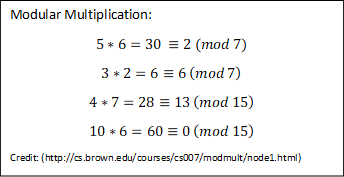
\includegraphics{images/modmul.png}
    \caption{Modular multiplication} \label{modmul:fig}
\end{figure}
Modular multiplication is pretty straightforward. It works just like modular addition. You just multiply the two numbers and then calculate the standard name. Examples for Modulo 7 and 15 can be found in Figure \ref{modmul:fig} 
Why modular multiplication is expensive? Because we have to take the modulo many times which is as expensive as division. Division is the most expensive integer operation exists, and  therefore we don’t want to do many divisions. So, one way to do this is by multiplying and multiplying and doing the modular reduction at the end, but the problem is the runtime of multiplication grows exponentially with the number of the multiplicands. 
Other way is with each multiplication do a  \( mod n \), but the numbers grow longer and longer, and the runtime gets higher and higher, so we can’t do that either. 
\begin{figure}[H]
    \centering
    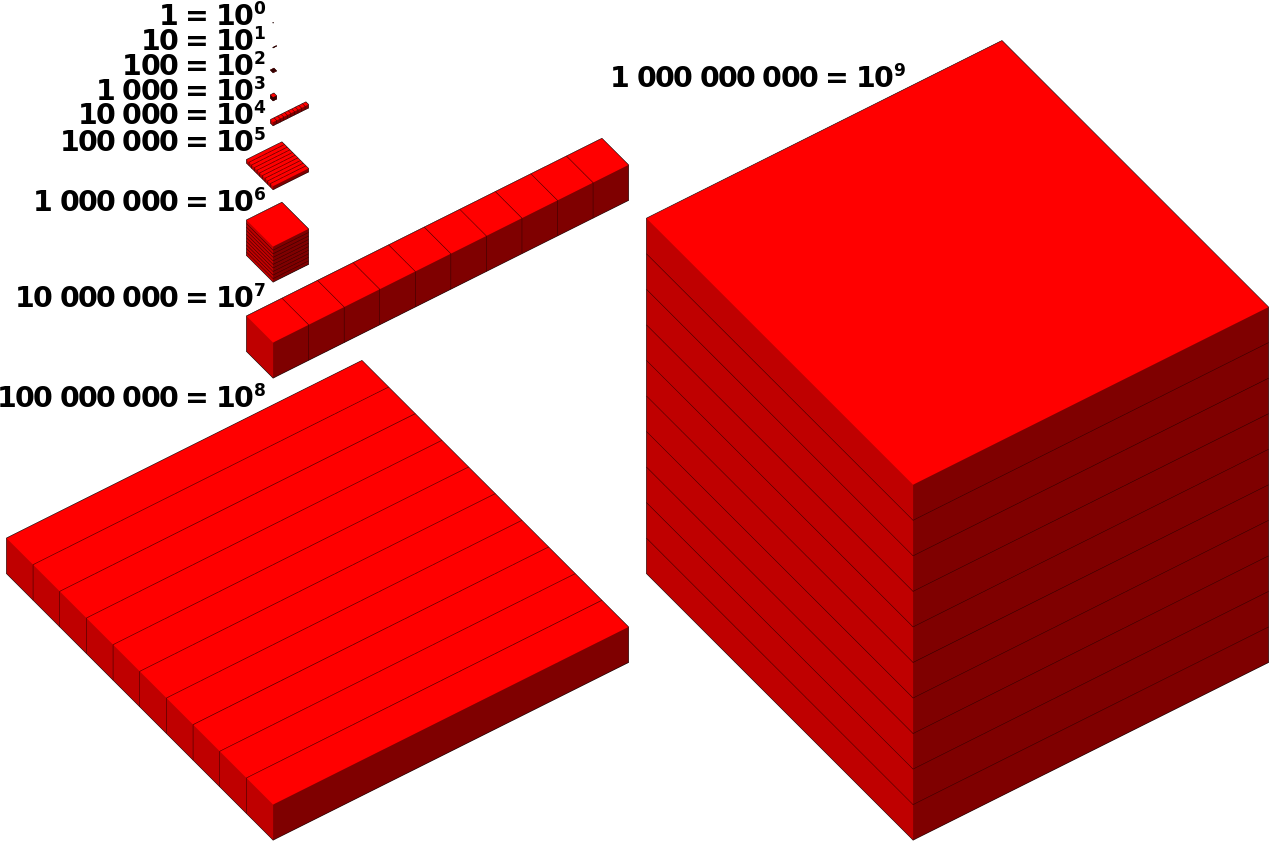
\includegraphics[scale=0.25]{images/vispow10.png}
    \caption{Visualization of powers of 10 from one to 1 billion.} \label{vispow10:fig}
\end{figure}

So, as we discussed in the last chapter, the slowest and most trivial way of implementing modular multiplication is just to take $g$ and multiply it by $g$, by $g$, by $g$ ($e$ times) \(g^e mod n\) and every once in a while doing modulo n, either every multiplication or just in the end. The problem with this was that if e is a number that consists of 1024 bits, then the worst case number that we might need to multiply $g$ is \( 2^{1024} \) which is a lot, we don’t want to do that.

\section{Efficiently Implementing Modular Exponentiations}\label{c1_basicformatting:sec}

There are two ways of making this faster, and these two ways are either performing fewer modular multiplication (instead of  \( 2^{1000} \)  we would like to do 1000) and we also want the modular multiplication to be less expensive. The best case, would be same as regular multiplication over integer. These two ways will reduce the cost of modular multiplication and modular exponentiations, and this is something we really want to do to make RSA work on a device.

So, assume we are engineers, we want to implement modular exponentiations very cheaply. The right thing to do is of course to use some crypto library, but let’s assume that’s not possible, we are inventing the new CPU or something. So, there is very serious book online called the handbook of applied cryptography (Figure \ref{appliedCrypt:fig})~\cite{katz1996handbook}. The book is like a phone book or a recipe book, and is filled with algorithms, proofs and equations you need for cryptography. Chapter 14 deals with efficient algorithms for multiplicative proofs. The book contains the ways to do modular exponentiation: very cheaply, more cheaply and the old fashion approach. 

\begin{figure}[H]
    \centering
    
\includegraphics{images/appliedCrypt.jpg}
    \caption{Cover of the handbook of applied cryptography} \label{appliedCrypt:fig}
\end{figure}

The following approach is called the left to right binary exponentiation, also known as square multiply.
\begin{figure}[H]
    \centering
    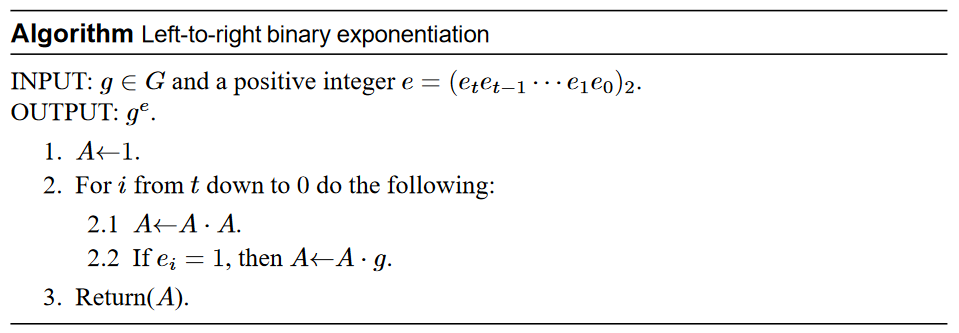
\includegraphics[scale=0.4]{images/ltrbe.png}
    \caption{The pseudo-code was taken from the handbook of applied cryptography, page 615.} \label{ltrbe:fig}
\end{figure}

The inputs are $g$ (we want to raise g to the power of $e$, \(g^e\)) and \(e\) which is a bit string of $t$ ($t$ bits), in the book its $t+1$ (see Figure \ref{ltrbe:fig}). The most significant bit is always $1$, because there is no logic behind raising something to the power of zero. In this algorithm in the end \(A\) will be the result of $g$ raised to the power of $e$. 
In the beginning we set $A$ to be equal to $1$, and go over the bits from left to right (from the most significant to the least). Each time we do square ($A$ equal $A$ times $A$, $A=A*A$) and multiply but we don’t always multiply, we do it sometimes. If the current bit is $1$ (the \( i^{th}\) bit) then we multiply by $g$, $A=A*g$. This is the algorithm. Now, what happens when we do a squaring operation downstairs? What happens to the exponent upstairs? Its multiplied by $2$. So \({g^{e}}^2 = g^{2e} \)  and  \(g*g^{e} = g^{e+1} \). Now, we can think of a binary string, you can write down the bits using shifting (multiplying by $2$ is shifting) and adding $1$ is just putting one in the place.
So how many modular multiplications will be performed in order raise g to the power of $e$ (the string is of length $t$)? The answer is \(O(t)\) What is the base case - lowest amount of multiplication that will be performed? the answer is $t+1$, the first bit is $1$ (most significant) so we do step 2.2 one time and all the rest of the string is zeros, and each time we do step 2.1. What is the  highest amount of multiplication that will be performed? Answer: $2t$, if all the bits $1$ I do each time $2$ multiplications (step 2.1 and step 2.2). Anyway, this is \(O(t)\).
So, instead of \(2^t\) as in the old algorithm we performed at most $2t$ multiplications. 
Lets review an example. Lets calculate \(7^6=7^{(110)}\) in the group \( \mathbb{Z}_{15}={1, 2, 4 ,7, 8, 11, 13, 14} \).
\begin{enumerate}
	\item  \(A = 1 = 7^(0) \)
	\item  \(A = A*A = 1 = 7^{(0<<1)} = 7^{(0)}\)
	\item  \(A = A*7 = 7 = 7^{(0+1)} = 7^{(1)}\)
	\item  \(A = A*A = 4 = 7^{(1<<1)} = 7^{(10)} \)
	\item  \(A = A*7 = 13 = 7^{(10+1)} = 7^{(11)} \)
	\item  \( A = A*A = 4 = 7^{(11<<1)} = 7^{(110)} \)
\end{enumerate}
Are there any ways doing it even faster? the answer is yes we can open the handbook of applied cryptography and find some others.
The general thought of these algorithms is that we do some precomputation. In RSA there is a public number that you know that you are going to start, so g is known number, we don’t care what $g$ is. So if we know what g is we can prepare all sort of lookup tables, in the window method we take each time three bits at the same time, and instead of doing \(A*g\) we do\( A*g*g\) or \(A*g*g*g\) .. (8 values we can use), and instead of \( A=A*A\) we do \(A=A*A*A\) and so on, this is the sliding window. There is binary method, you can just look at the book and find out (page 616 algorithm 14.83, in the handbook of applied cryptography). So this is how you reduce modular multiplications and we can assume that any reasonable crypto implementation is not doing the naive method. It will use the left to right or the right to left which is basically the same idea or one of the window methods.

But what if we want the modular multiplication to be cheaper? There is a way and it's called the Chinese remainder theorem (CRT)~\cite{dingyi1996chinese}, which is called after Sun Tzu Suan, that was a teacher from the fifth century and he wrote a book that contained all sorts of riddles and questions. And there is the riddle: 

"there are certain things whose number is unknown.  If we count them by threes we have two left over; by fives we have three left over; and by sevens, two are left over. How many things are there?" 

The answer is 23 and how it was discovered? Brute-force.
So the CRT states that you have to have an equation set over modulo other multiplicative group such as this, you can solve it modulo $p$, you can solve it modulo $q$, this is more general theorem. You can solve it modulo the underling primes then combine them, and if there is only one solution in each of the sub-groups there is only one solution in the big group. What this means is that if we want to do modular multiplication in this big field modulo $N$, we can actually do the computation in modulo $p$ and modulo $q$ and then we can combine them together. Why does this help us (we have to do 2 operation instead of one)? Answer: to do exponentiation in CRT we take our  big number and do modulo $p$ and again modulo $q$ and then there is a CRT step. So these two modular exponentiations, what is the size of the operand they are using? Assuming that $p$ and $q$ are of the same size? Let’s say $p$ and $q$ is 1000 bits so the size of $n$ is 2000 bits (we add the number of bits of each number in the multiplication).  So each number in the multiplicative group is about 2000 bit because its mod $N$, so multiplying two numbers is going to be multiplying two numbers which are 2000 bits. If we reduce it to modulo $p$ and modulo $q$ my numbers are going to be half the size (1000 bits). So if we take a multiplication and now we will multiply two number that are half the bit length what is the speed improvement I get? It's times 4. Instead of one modular exponentiation we have one baby modular exponentiation which costs me quarter of the time and another one which cost me quarter of the time and a step (the CRT step which is a modular multiplication of the two). How much we spent in total? Answer: a bit more than half the time, twice speedup. Why can’t we do that further? Divide $p$ and do it again? Answer: because it’s a prime number ($p$ and $q$) that’s the whole point. So if you do the CRT each modular exponentiation will take less time. 

Now there is a really nice trick, to make modular multiplications very cheap and this actually makes modular multiplications as cheap as regular multiplication. So, magic, what is the problem? Multiply two number is pretty easy but the problem is reducing after multiplying. So what if there is a way of doing modular multiplications without the reduction step? So in 1985 a genius mathematician called peter Montgomery published a paper called "modular multiplication without a reduction step" ~\cite{warren2013hacker}\footnote{https://www.hackersdelight.org/MontgomeryMultiplication.pdf}. So the idea is there is a kind of magical world called the Montgomery representation and you take your number and you step into the Montgomery world where modular multiplications do not require reducing step and when you finish you step out of this world and you are back with your result. It’s still cost you like a multiplication but it doesn’t cost you the extra reduction step.
So, what is the idea of the Montgomery reduction? we want to calculate \(g^emodn\) and to do that we need to pay a lot of modular reduction which we  don’t want. So, the first thing we do is enter the Montgomery representation and we do the Mont(\(g^e\)) and each one of this multiplication steps is going to be about as difficult as regular multiplication (Figure Figure \ref{montg:fig}). When we  finished with this we exit the Montgomery representation and then we have our result. Entering and leaving the Montgomery representation costs as much as modular multiplication but in the middle it's as cheap as regular representation.

\begin{figure}[H]
    \centering
    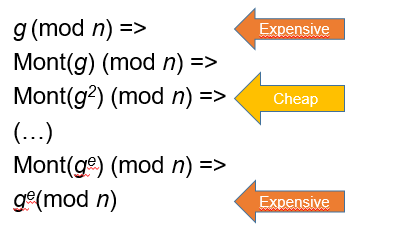
\includegraphics[scale=0.7]{images/montg.PNG}
    \caption{General sketch of Montgomery Exponentiation} \label{montg:fig}
\end{figure}

Now lets review how the Montgomery Exponentiation works inside
\begin{enumerate}
	\item  Choose a value R, \(R>n\), which is easy to use (usually a large power of 2)
	\item  \(Mont(a)=a*R(mod n) =^{def}  a(mod n)\)
	\item  \(Mont(ab)=a*b*R(mod n)=\underline{a}*\underline{b}*R^{-1} (mod n)\)
	\item  \(... \)
	\item  \( = (\underline{a}*\underline{b} + (\underline{a}*\underline{b}*n’(mod R)*n))/R(modn) \) \newline
	// if this is more than n, subtract n
	\item  \( A = A*A = 4 = 7^{(11<<1)} = 7^{(110)} \)
	\item  Result: Instead of modular reduction, we only (sometimes) subtract
\end{enumerate}

The first thing to do is to choose a very large value $R$. which is larger than $n$ and should be easy to use ($a$ large power of 2) for instance 1 and 1000 bits of zero. What does it mean easy to use? To multiply and divide by a power of 2 you just shift left and right. To calculate the modulo of very large number that is a power of 2 you do bitwise and with this large power of 2. if $R=100000$ and $x = 10101010101110$ so to do  modular reduction we just take the lower bits which are 01110 in this case. So we see its very cheap operation with $R$, but $R$ is not useful outside the situation. So to enter the Montgomery representation we are going to multiply by $R$, this multiplication is modulo $n$, this is a bit expensive. So let me ask you, how do I know that $R$ is inside the multiplicative group? How do I know that multiplying by $R$ doesn't throw me outside of mod n? The answer is: how do we know that 2 is inside the group? Because what is this group? This group is a multiple of two prime numbers, and they are odd. Thus 2 doesn't divide either one of them so 2 is in the group and \(2*2*2...2\) is in the group. We call the new number \underline{a}. The idea is that the numbers in the Montgomery representation is cheap so how is it cheap with \underline{a} If we multiply a and b in the montgamery representation It will be: \(a*b*R mod n\). but if I want to do that using \textbf{a} and \underline{b} we  get: \(\underline{a}*\underline{b}R^{-1}\)mod $n$ because of the extra R. So every time we multiply two numbers we need to take out the extra R. Inverting $R$ is just using GCD and can be done before we start the computation. There are much more derivations made to get to  \((\underline{a}*\underline{b} + (\underline{a}*\underline{b}*n’(mod R)*n))/R(modn) \). \underline{a}*\underline{b} is just a single multiplication.  \underline{a}*\underline{b}*n’(mod R) - Notice that \(modR\) is a cheap operation because $R$ is 1 with lot of zeroes. (n prime (n') is just precomputed number doesn’t really matter to us). Then we multiply it by $n$ (another multiplication) and then we divide it by $R$ which is also simple operation. So, we have 4 multiplications and we need a modular reduction which is the core problem. Montgomery proofed that this sum is no more than \(2^n\). So how do you do a reduction if the number is between 0 to \(2^n\)? you put an if statement. If $x$ is less than $n$ you do nothing, if $x$ is larger than $n$ you subtract from the number n. So now, instead of division we do a couple of multiplications over integers which is not such a big deal and then we sometimes subtract. This is a lot cheaper than the regular option and is widely used. Notice the if statement in the algorithm, it is changing the execution time and might enable a timing attack.

\section{Temporal Side Channel on RSA}\label{c1_basicformatting:sec}

Lets review a do temporal side channel attack on RSA. Kocher described this attack on his paper in 1995 among other things. If the RSA runs slower than there are more subtractions and by timing the execution we can recover the key. So how to do this? How to recover the key by timing the execution? There was a fantastic paper "A Practical Implementation of the Timing Attack"~\cite{dhem1998practical} which the remainder of this section is based on. So what is the game here? Assume we are an attacker who wants to commit a timing attack at the secure implementation of RSA. We have a device (a smart card) and sending him a request, for instance "please allow to pay 1000 dollars to Alon" (figure \ref{smartcard:fig}). The smartcard check that I have 1000 dollars in the bank account and then it replies "I approve this transaction and sign it" so this card has stored value inside which means he has money inside. we would like that if we request "pay Alon 1 million dollars" the smart card will say "I don’t have enough funds I am going to refuse". As an attackers we would like to be able to sign any message we want, mainly messages like "please send yosi 1 billion dollars". The smartcard will not allow it but if we got the private key (signing key) we could sign whatever message we want. So we send the smartcard a message that is unsigned and he in return sends back a signature which is the response signed with the private key: \(m^s mod n\) where s is the secret key. So as an attackers we can send as many queries we want and we  allowed to recover the responses (the signatures). The goal is extract the secret key. 

\begin{figure}[H]
    \centering
    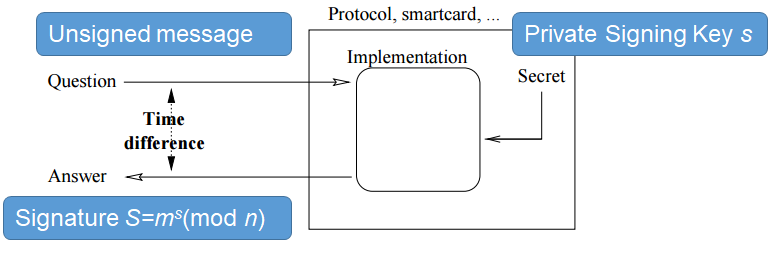
\includegraphics[scale=0.4]{images/smartcard.png}
    \caption{The timing attack principle} \label{smartcard:fig}
\end{figure}

So, let’s look a bit closer in the attack model, what messages we can send to the smartcard? Can we send any message we want? The answer - we can only send valid messages, if the message is not valid the smartcard will just throw them away. So, this is somewhere in the scale between the weakest model and the most powerful model. In this scenario the most permissive attack model is known plain text. Known plain text means that we can see the messages as they go in the smartcard but cannot change them. So the next thing is chosen plain text, we can’t  just chose any plain text, it has to follow a certain rule. The next thing is completely chosen plain text which doesn’t enforce any rules, and the last thing is adaptive plain text which means we can look at the response and we can think the next that we will send. So, what is the attack model, we send requests, the smartcard is signing them, and we get the responses and also we know that the smartcard is using Montgomery RSA because it is a reasonable assumption. So how to use it to extract the key? So we are going to use a method named "Vaizata" method which can be found in the DPA handbook. This is a general way of performing a side channel attack using statistics. \newline

\underline{The “Vaizata” Method}
\begin{itemize}
	\item Make a simple assumption about the implementation
	\item Guess a little part of the key
	\item Make hypothesis about the effect of the guess on the execution
	\item Classify the measurements according to the hypothesis
	\item If we guessed right, the classification will be statistically meaningful
\end{itemize}

How does it works? First, we make a simple assumption on the implementation, an assumption could be: We assume that the implementation run on software (the other possibility is the hardware) what does it gives us? Software is executed serially and in the hardware it’s not the case. We can assume for example that the key is stored in a flash memory on the device, and every time we need to use the key you need to read the flash memory. How can we find that this is the case? How can we find first of all that a device is on the hardware or on the software? One way is to look at it, We can open the screws and look with a microscope, We can go to this wonderful website called “I fixed it”. They disassemble all sorts of devices and share this information. What is the sign that the device is using software? If there is an update on the firmware, because when it wakes up it needs to find out what software to run. We can say this device uses memory, We can also say things about when the device is doing the encryption. So let’s assume the device under test is a remote controller. Inside the controller there is a secret key stored and also a counter. Whenever the button is pressed the remote controller constructs a package containing the serial number of the controller, the counter and whatever Boolean state of the button (which ever button was pressed). Then it sends it to a car and the car decrypts it. Why by the way do we need a serial number? Each ECU in the car has program to accept remote controls. So why do we need the counter? Without the counter an attacker can repeat a message sent from the remote controller to the car only by reading the messages and sending them again. What happens when you press the button and the car is in the train station? The counter in the remote controller is out of sync with the counter in the car, there is a window of counter values the car will accept, if its closed the car will open without complaining. If it’s a little closed we will need to press the remote control twice and when the car will see consecutive values it will open, but if it is too far it won’t open. let’s assume We can find out when the controller is transmitting (it is a very intensive operation that takes battery life and also radiates). So we know the moment in time when it is transmitting, did the encryption happened before or after the transmitting? Answer: before. Let’s assume that the counter stored in the memory, let’s say we found the moment in time when the chip is reading from memory, did it happen before or after the encryption? Answer: after, because we need the counter to be included in the message that will be sent.We can also make more assumptions such as "the AES uses an 8 bit data pack or 16 bit or 32 bit", some of these assumptions might be wrong but the “vizata” method will help us to find out if they are wrong. 

So first of all We make a simple assumption, assume that the smartcard is using left to right binary exponentiation using Montgomery and this is a very reasonable assumption because everybody is using this method. The next thing to do is recursively (or inductively) guess a little part of the key. if we guessed the whole password it would take us exponential time but if we could guess a small part of the key each time it would take a linear time. So, we will try guess small parts of the key first, maybe the simplest thing to explain is guessing one bit or a single character but lets say we are guessing a small part of the key. So now we know the beginning of the key and there is a little part we don’t know. So the next step, we need to make a guess about what kind of an effect our guess is going to have on the computation. We can say, for example, if we will guess the bit correctly than something will happen to the computation, if we will guess this key bit correctly it will take more power/take longer time/connect to the network more often, some kind of phenomena we can measure. So, in our case what is the only thing we can measure? Answer: time. we assume that if there is a Montgomery reduction in the calculation of this bit than the entire computation is going to take a little more time.


SO what is going on here? There is a very large computation here, we were able to guess the beginning of it but not the end of it. Now we are going to classify the measurements according to our hypothesis, in this case two groups (with or without Montgomery computation). If we guessed correctly then it will take longer to the group we said it will take longer. If not, it might take less or more, we don’t know. If we guessed correctly, the groups will have meaning, means will will be able to statistically tell apart the set of the measurements that will take a longer time and the set of measurements that will take less time. We are going to guess the left most bit of the key, there are only two options, most of the cases it will be 1. The next bit? 1 or 0. Now, we can simulate the running of this algorithm with our guess, not all the key but only the part we know and if there is going to be Montgomery reduction. So assume we have g, e and N. The device under test is calculating \(g^emodn\) where g came from? Supplied by the attacker. What about of e? secret we want to discover (\(e_t,e_{t-1},..,e_0\)) What about of N? public variable (known). The first thing it does, it enters the Montgomery representation. This information of how to enter the Montgomery representation is known to the attacker. It starts with g, then g becomes Mont(g), the attacker can also do it. First \(A=1\), than \(A=A*A\) the next thing is \(A=A*g\) because we know that the most significant bit is 1. The next step is \(A=A*A\), now what is next? It depends, if \(e_{t-1}\) = 0 then \(A=A*A\) (skipping to next bit). Else if \(e_{t-1}\) = 1 then \(A=A*g\). What happens next now we don’t know. We can run both calculations, in particular we can find out if there was a reduction step in two optional operations. There are 4 option either one containing reduction step, neither or both. We can know exactly, assuming we make a guess on \(e_{t-1}\), if there is going to be an extra reduction step. We know enough to guess, if we guess correctly, we can know if there will be reduction step because we can calculate all the alternative options completely. So, lets do this now, we have many different g’s, we have repeated this step many times, and for each of these g’s we know if there is going to be an extra reduction step. So, now let’s see how we do an attack using this. So, there is private key s, public key v and signing operation \(m^s mod n\). 

We begin the attack with a bag of messages, all of them are valid, and we send them to the device under test (DUT). The DUT signs these messages (k messages), and for each one of the messages we get a trace, which is the data we collected using the side channel attack in this case it is only the time. now we have a vector of size k and each element in the vector is the time it took to sign the message. Now, we are going to try to guess \(s_t,s_{t-1}\)  
\((s = s_t,s_{t-1},s_{t-2},…,s_0)\) and try to discover \(s_{t-2}\). 

So for each of the messages and each key guess we are going to simulate the computation as far as we already know and in addition for the parts of the key we don’t know we are going to simulate twice, why? One with a 0 and one with a 1. We are going to find out where the extra reduction step happens. If the next bit is 0, some of the messages have extra reduction we classify the message into two bins, those who got extra reduction and those who didn’t. But maybe the key is not 0 maybe its 1. So we can simulate the same thing with the next bit as 1, and find out different set of messages with an extra reduction step. We can’t find what the bits are but we can make a guess and simulate on both 0 and 1. So, now we divide our traces into two groups in 2 different ways, if the next key bit is 0 \(m_1,m_2,m_4,m_5,m_7\) got extra reduction and \(m_3,m_6,m_8,m_9\) didn’t. If the next key bit is 1: \(m_2,m_3,m_5,m_8\) got extra reduction and \(m_1,m_4,m_6,m_7,m_9\) didn’t (Figure \ref{extraRed:fig}). 


\begin{figure}[H]
    \centering
    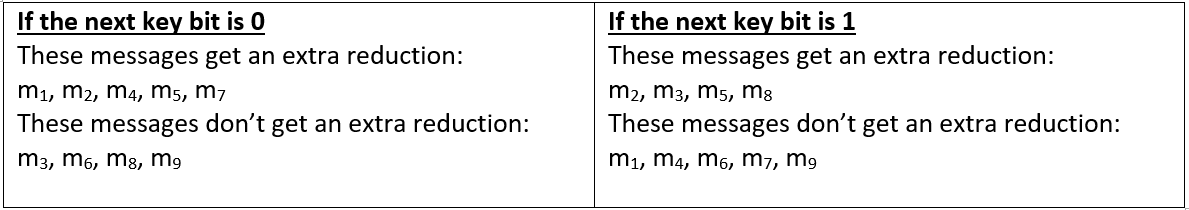
\includegraphics[scale=0.3]{images/extraRed.PNG}
    \caption{Key bit guess simulation} \label{extraRed:fig}
\end{figure}

If we guessed correctly what can we tell about the messages that got extra reduction? Answer: the runtime will be a little longer if we guessed the key bit correctly and If we guessed incorrectly it means we divided into two random groups which means the runtime will be similar in both groups. So if we guessed correctly the difference of runtime between the groups will be measurably different. So now we are going to change the discussion about the messages into the traces.

\begin{figure}[H]
    \centering
    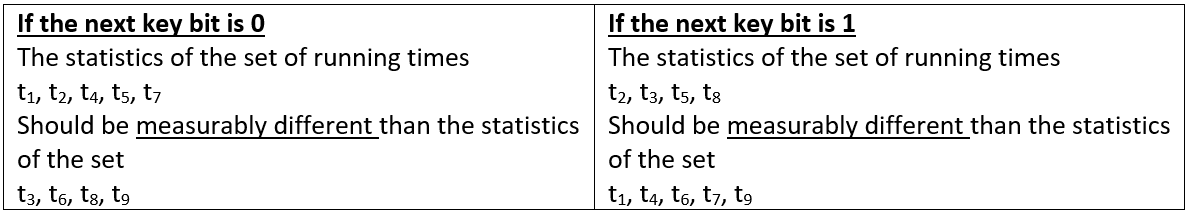
\includegraphics[scale=0.3]{images/extraStat.PNG}
    \caption{Guessing correctly the key bit makes the statics measurably different} \label{extraStat:fig}
\end{figure}


if the next key bit is 0 then the statistics of the runtimes of 0 bit with extra reduction are going to be different from the runtimes of 0 bit without extra reduction. If we guessed wrong the runtimes of 1 bit with extra reduction will be different from 1 bit without extra reduction. Notice that we are not saying average or mean anywhere, because they are not required, it could be the variance changes or something else, the point is that there is some kind of difference that we can measure. So, how can we find out which of these two divisions is the correct one? Answer: we have two divisions of k traces, we measure distance of means. We are going to calculate the mean runtime of each part (0 bit with or without the extra reduction and 1 bit with or without the extra reduction) and subtract between with/without extra reduction in each bit guess. If there is a large distance of means of the 0 bit guess as oppose to the 1 bit guess than probably the splitting of traces in the 0 bit guess is more meaningful than 1 bit guess, if we are able to split meaningfully then we guessed the key correctly. 
Now, let’s go back into statistics and talk about the T-test~\cite{wikittest}. The T-test was invented by William Sealy Gosset~\cite{wikigosset} who was a chemist who worked for a very famous brewery in Ireland (Guinness). So, what is the idea? We have two populations that are different in some way. There are two kinds of t-tests, pair T-test and unpaired T-test. what is the paired T-test? lets assume we claim that we are going to a tree and we taking the leaves that fall off the tree. We notice that the leaves that fall on the south side have less mold that on the north side, why is that? Because there is more sun on the south side that is drying the leaves. 

How do we prove our theory? We send our undergrad research assistant to collect a bag of leaves form the north side and a bag of leaves from the south and now I tell the undergrad to count the percentage of mold in the southern and northern leaves. When the undergrad comes back, very exhausted, he provides us with an excel file that have 1000 leaves from the north side and 1500 from the south side. Now we want to prove our theory, each one of the leaves has a mold, We want to prove that there is a statistical difference between the two groups, this is the unpaired T-test. What is the paired? It is when we ae talking about something which we can identify as pairs. For example, we are developing a cancer medicine and we want to test it. Now, we don’t take any undergrads but only very sick mice with cancer. We measure the weight of the tumor in order to have a list of 100 mice and tumors. Then we divide them into two groups, one we treat with my medicine and the other we don’t. In the end of the experiment, we measure the tumors again, but now each measurement is a pair, one before treatment and one is after. And we want to say that the size of the tumor is smaller after the treatment. 
Now let’s review the student's unpaired T-test demo in matlab. The mat in matlab is for matrix, we can define matrix like this:

\begin{figure}[H]
    \centering
    \fbox{
    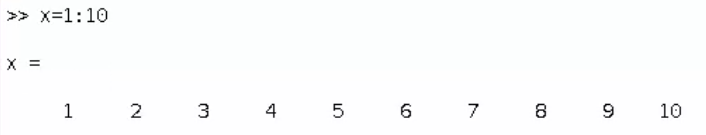
\includegraphics[scale=0.5]{images/defmat.png}}
    \caption{Defining a matrix of size 1x10 with increasing numbers from 1 [1,2,3,…,10]} \label{defmat:fig}
\end{figure}

\begin{figure}[H]
    \centering
    \fbox{
    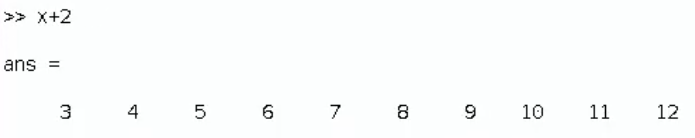
\includegraphics[scale=0.5]{images/defmat2.png}}
    \caption{Adding the matrix with 2 increases all the numbers in the matrix by 2 (Same with multiplication and log)} \label{defmat2:fig}
\end{figure}

\begin{figure}[H]
    \centering
    \fbox{
    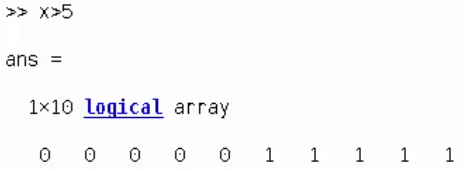
\includegraphics[scale=0.5]{images/defmat3.png}}
    \caption{\(x>5\) will result with logical array [0, 0, 0, 0…, 1, 1, 1, 1]} \label{defmat3:fig}
\end{figure}

The function randn(1) which creates normally distributed random variable which follows a Gaussian distribution which means the variance is 1 and the mean of 0. What is the minimum value this function will output? Answer: None, but statistically the value is closer to 0. How can we create a random variable with mean different from 0? Answer: add the mean, if we want mean N. we will do $N$ + randn (1). We can even create a vector of randomly chosen numbers using randn (1, 5) + 5 : [4.9369, 5.7147, 4.7950, 4.8759, 6.4897] and if we will do randn (1, 5)*.1 + 5 the numbers will be even closer to 5.
So, now we are ready to try the student T-test.

\begin{figure}[H]
    \centering
    \fbox{
    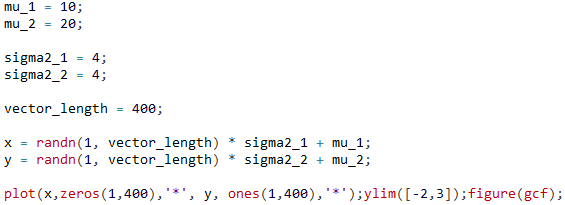
\includegraphics[scale=0.6]{images/defmat4.png}}
    \caption{In the code, 2 vectors are created - x and y in the same size (which is not obligatory), $x$ will be randomly distributed with a mean of \(mu_{1}\) and variance of \(sigma2_1\) and vector $x$ is going to be random distributed with a mean of \(mu_2\) and variance of \(sigma2_2\). Then there is a code for plotting both vectors (in different colors).} \label{defmat4:fig}
\end{figure}

\begin{figure}[H]
    \centering
    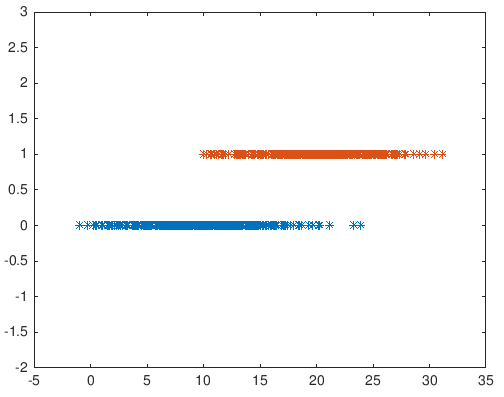
\includegraphics[scale=0.6]{images/defmatplot.png}
    \caption{Plotting of the vectors for \(mu_1 = 10, mu_2 = 20\)} \label{defmatplot:fig}
\end{figure}

Looking only on the graphs can we say they are from the same distribution? Answer: we can't be sure.
We want to run the T-test to find out if they are statistically significant. There is a hypothesis and we need to either reject or accept the hypothesis. If \(H_0\) than they are from the same distribution and if \(H_1\) than they are from different distributions. If we run the code the result will be that they are of different distributions with 0.959 certainty. Each time we ran we can get different results, if the certainty is smaller than 0.95 in matlab, the hypothesis is rejected. How can we make it more difficult for the ttest2? Answer: if we change \(mu_2\) to 11, than they will be very close distributions. 

\begin{figure}[H]
    \centering
    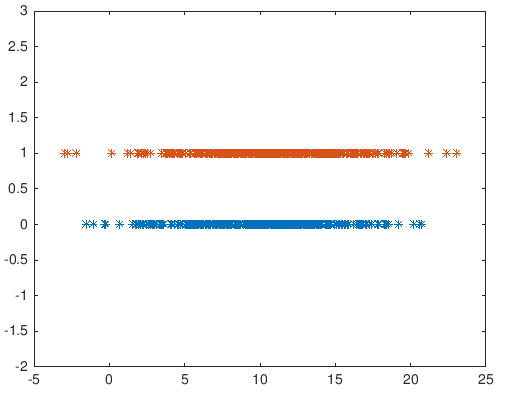
\includegraphics[scale=0.6]{images/defmatplot2.png}
    \caption{Plotting of the vectors for \(mu_1 = 10, mu_2 = 11\)} \label{defmatplot2:fig}
\end{figure}

How we as attackers will handle this situation? Answer: run many times. So we change the vector length (such as 50000). There is something called power analysis, which means given these parameters (mu and sigma) how many measurements you need to run to be sure with 95%.
As engineers we don’t really care about T-tests, we have a budget of measurements and we just take the one with the larger mean distance, but what if we are wrong (guessed 1 instead of 0)? Answer: after we guessed one bit wrong all the bits afterwards are wrong because they are simulated wrongly.
So, how can we simulate a full attack? If we guessed 1 bit using the differences of means then we continue to the next bit in linear time. Lets review  a figure from " A Practical Implementation of the Timing Attack" which you are encouraged to read.


\begin{figure}[H]
    \centering
    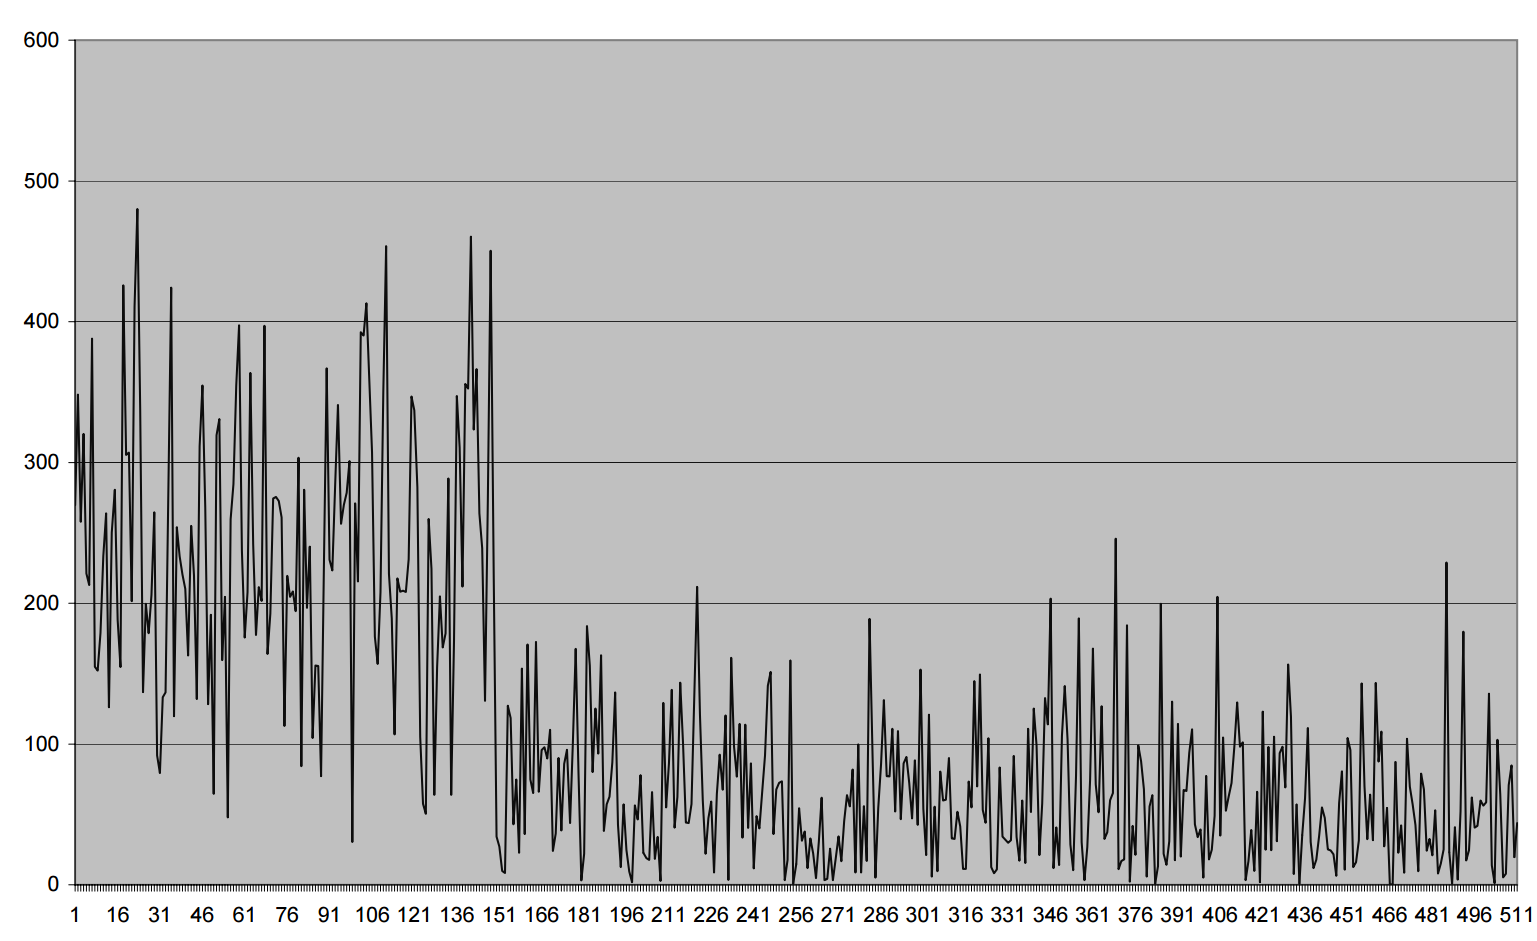
\includegraphics[scale=0.25]{images/figpita.png}
    \caption{x axis – is the bit index from right to left (the left most bit is known to be 1) and y axis – is the distance of means we chose (some times its 500 or 100 but after 151 the distance of means is a lot smaller which means we guessed a bit wrong). How to solve it? Answer: go backwards and backtrack.} \label{figpita:fig}
\end{figure}

Now lets talk about counter measurements. When Kocher announced the attack to the cipherpunks mailing list there was kind of discussion about it. Here is a message (Figure \ref{paul:fig}) from there that was sent by Ron Riverst. He was replying to William Simpson, who was the author of Photuris which is related to the IPsec protocol and was used for kits change in the IP protocol. 

\begin{figure}[H]
    \centering
    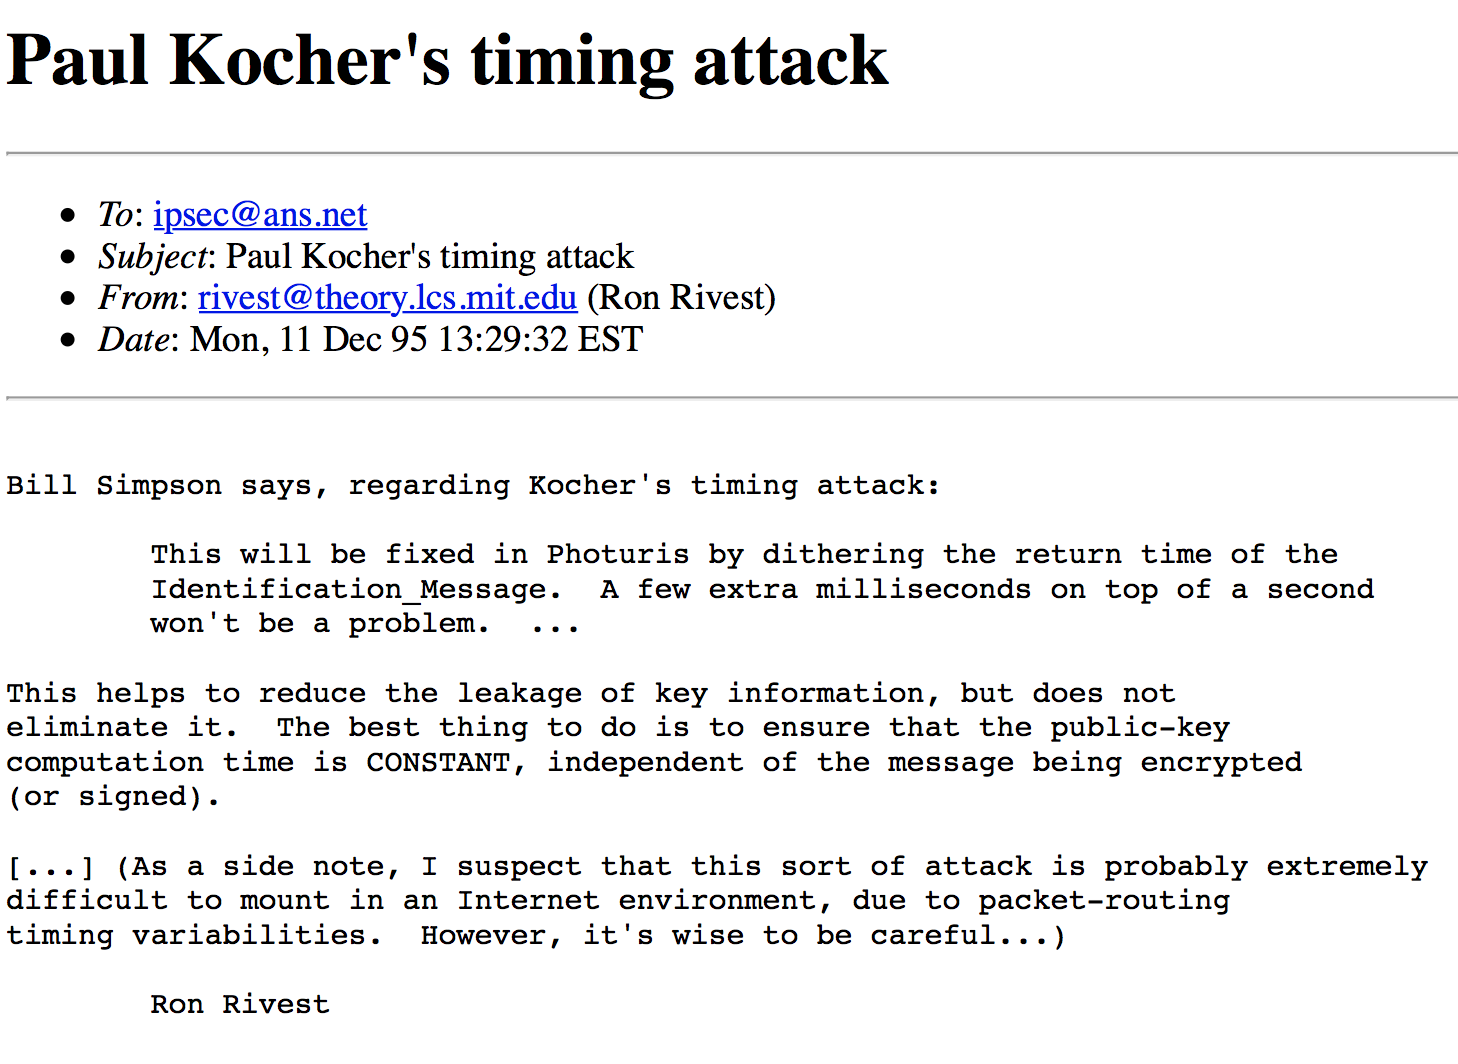
\includegraphics[scale=0.25]{images/paul.png}
    \caption{The message.} \label{paul:fig}
\end{figure}

When he read that this attack can attack Photuris, Bill replied: don’t worry this will be fixed in Photuris. How to do this? By dithering the return time of identification message a few extra milliseconds. Which means he is doing mitigation, he is not adding a random delay because random is very expensive, he is going to finish the calculations and is going to look at the clock and exactly when the millisecond changes (or second) send the package. What does it mean? It means that since the beginning is random then he is going to add random delay. So, what Ron Rivest replied? It will reduce the data leakage but will not eliminate it. Why so? How the attacker will overcome this? Answer: he will need to measure more, this is network-based protocol, the attacker can measure many more times. He says, in addition, the public key computation time should be constant and independent from the message being sent. Ron Rivest suggest prevention as a countermeasure. So, what time it is going to be? Answer: the worst-case time. he adds a side note that this kind of attack is very difficult to mount in an internet environment due to packet-routing timing variabilities, however it is wise to be careful. Few years later a demonstration was presented over the internet, there were more measurements to counter the routing problem. Adding noise is sometimes the only thing that works, sometimes it works sometimes it doesn’t, if you add enough noise to delay the attack time up to a year the message might not be relevant by the time the attack succeeds.

So, lets talk about two counter measurements, which are preventions. The first one is called RSA blinding. RSA blinding is a prevention counter measure which actually works on average time and not worst-case time. we have secret key S and want to calculate \(m^s mod n\), and the attacker gives us m and we don’t want to leak s. We showed that with enough m from the attacker he will successfully retrieve s. 
So, how do we do blinding? First of all, we can do this even before the attacker arrives, we generate random $r$ and calculate \(r^v mod n\) and \(r^{-1} mod n\). these calculations are not reviling any secrets because v is the public key. The attacker gives us m, so we calculate: 
\[X = (r^v * m) mod n\]
\[Y = X^s = (r^v*m)^s = r^{vs}*m^s = r*m^s mod n \] 
\[ // v*s mod n = 1 mod n)\]
Now, $Y$ is leaking information because we raise a number to the power of the secret key, but $r$ is random number which the attacker doesn’t know so he can’t simulate the execution. How we remove r? We just calculate 
\[S = Y*r^{-1} = r*m^s*r^{-1} = m^s mod n\]
Why doesn’t everybody use it? Answer: because its expensive, 2 modular exponentiations instead of 1. Another problem is the random number generation, its hard to find random number generator. You can see RSA blinding in openPGP. 

Now lets review another countermeasure. It called square and always multiply (Figure \ref{saama:fig}). It is very similar to the square and multiply, just instead of only when \(d_i\) is 1 we will always calculate the multiply but the assignment will be only when \(d_i\) is 1. The problem with this is not the extra computation that came from turning sometimes to always. Speculative execution is always looking for instruction to execute, how does it decide if it will execute an instruction? If all its dependencies are met. If I say \(a = b*c\) and \(e = b*c\) they can run both in the same time. what happens is when the instruction brought to the CPU there is actually nobody is waiting for t, so as soon as it finishes to run the \(s =s *s mod n\) and \(d_i\) is equal to 0 it will just return s. Moreover, the compilers are also capable of detecting such cases and optimize them by dismissing the else statement. So if we have a very simple CPU with no speculative execution no compiler and we wrote it in assembly we wont be able to attack it, but we could use power analysis.

\begin{figure}[H]
    \centering
    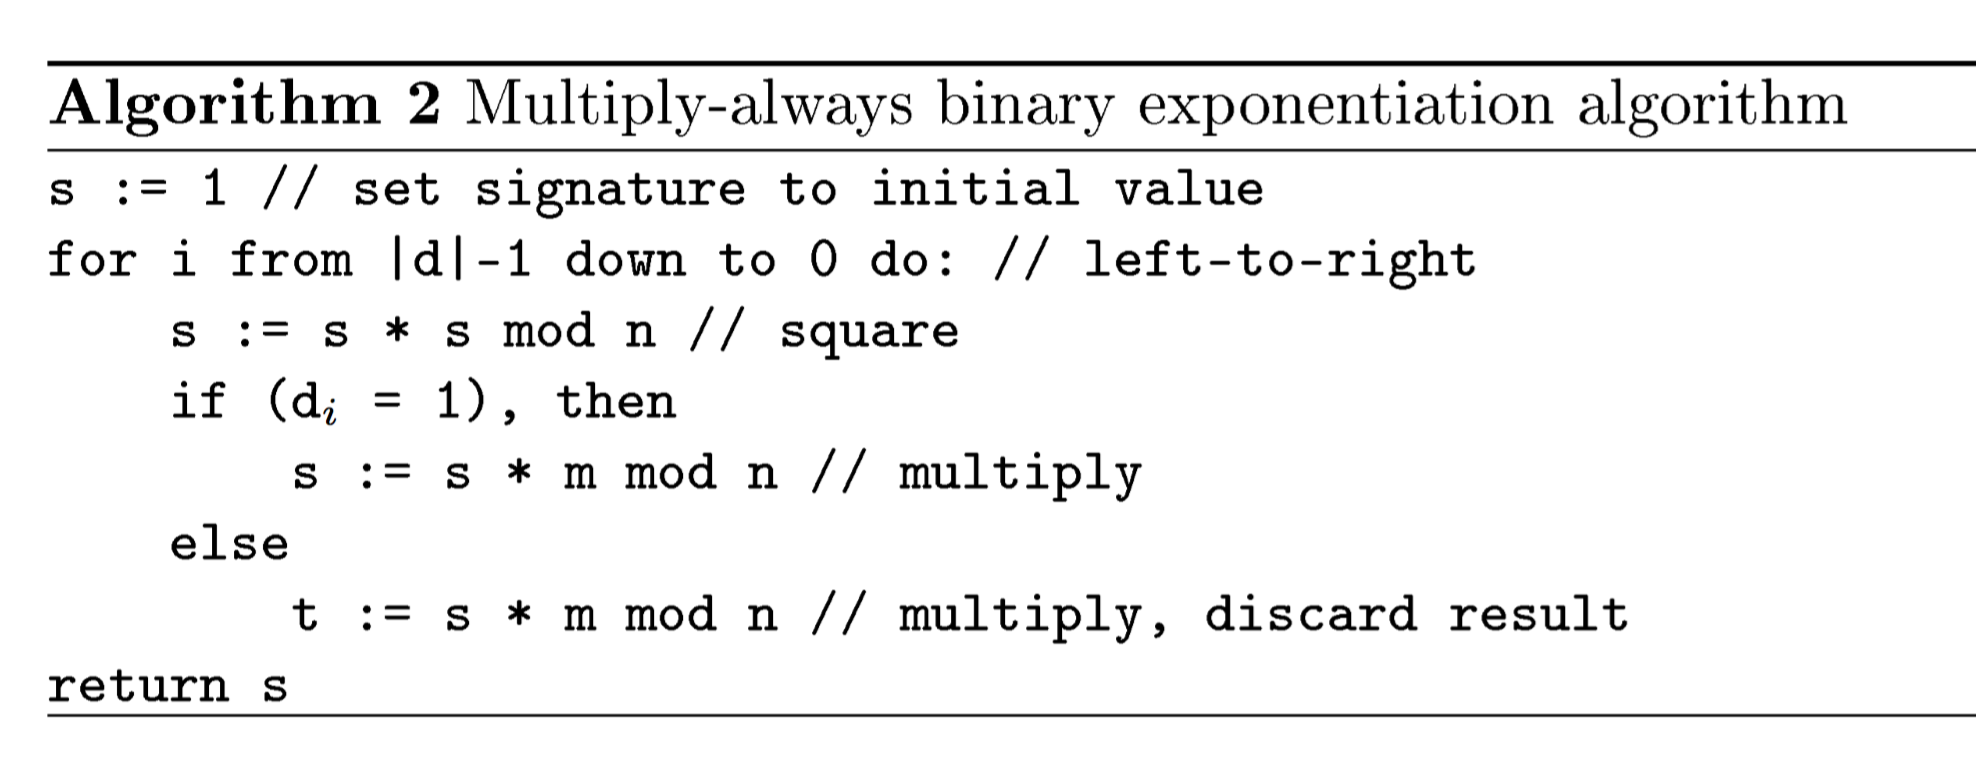
\includegraphics[scale=0.15]{images/saama.png}
    \caption{Square and always multiple algorithm} \label{saama:fig}
\end{figure}

If we run this algorithm as is, we have two places in memory for s and for t, every action we load s then multiply and then edit the memory of s, same goes in the multiply section. We load s and m then multiply and then store it in s. It’s always loading and storing s, but what happens when it goes to the else segment: it loads s loads m and then store into something other then s. So the power consumption is different between the store and the load. You can read more in the paper (“defeating RSA multiply-always and message binding” by Marc F. Witteman et al.~\cite{witteman2011defeating})

Side channel attacks can get not only computer secrets but human secrets too. What exactly is a human secret? Browsing history for example. How does the website figure out our browsing history? Theoretically, we can delete the history in the browser. But what happens when we click on a hyper link (blue link)? It turns purple after the click. So, there was a nice trick that websites used to do, they attached the link to an html element and added JavaScript code that at the change of the color can now update that you have visited the site. The world wide web consortium decide that it was a privacy leak and you are not allowed to read the color of an html element anymore. Now we can set the color but can’t read it. One of the speakers in the black hat 2013 used timing attacks to find out if a web site was visited or not\footnote{https://www.youtube.com/watch?v=KcOQfYlyIqw}. He also demonstrated how he can also use timing attack to read the user’s stream. 

\chapter{Writing \LaTeX{}}\label{cha:c1_firstchapter}

This document shows how you can get ePub-like formatting in \LaTeX{} with the \verb|memoir| document class. You can't yet export directly to ePub from writeLaTeX, but you can download the source and run it through a format conversion tool, such as \verb|htlatex| to get HTML, and then go from HTML to ePub with a tool like Sigil or Calibre. See \url{http://tex.stackexchange.com/questions/16569} for more advice. And they lived happily ever after.

\section{Basic Formatting}\label{sec:c1_basicformatting}

\paragraph{Comments.} If you want to just add a comment to a file without it
being printed, add a \lstinline[language=Tex]!%! (percentage) sign in front of
it. In the template files, you will find a number of such
comments as well as deactivated commands.

\paragraph{Bold formatting.} You can make your text bold by surrounding it
with the command \lstinline[language=Tex]!\textbf{}!.

\paragraph{Italics formatting.} You can make your text italic by surrounding
it with the command \lstinline[language=Tex]!\textit{}!.

\paragraph{Small caps.} You can change your text into small capitals by
surrounding it with the command \lstinline[language=Tex]!\textsc{}!.
    
\paragraph{Text em dashes.} Em dashes are used to connect two related sentences.
There is no space before or after the em dash. Within the template, use the
command \lstinline[language=Tex]!\textemdash{}! instead of using the dash you
copied over from your text file. This will also take care of issues relating to
line breaks.

\paragraph{Paragraphs.} Paragraphs are handled automatically by leaving an empty
line between each paragraph. Adding more than one empty line will not change
anything\textemdash{}remember it is not a ``what you see is what you get''
editor.

\paragraph{Empty line.} If you want to force an empty line (recommended only in
special cases), you can use \lstinline[language=Tex]!~\\! (tilde followed by two
backslashes).

\paragraph{New page.} Pages are handled automatically by \LaTeX{}. It tries to
be smart in terms of positioning paragraphs and pictures. Sometimes it is
necessary to add a page break, though (ideally, at the very end when polishing
the final text). For that, simply add a \lstinline[language=Tex]!\newpage!.

\paragraph{Quotation marks.} In the normal computer character set, there are
more than one type of quotation marks. It is required to change all quotation
marks into \lstinline[language=Tex]!``\dots''! (two back ticks at the beginning
and two single ticks at the end) and refrain from using ``\dots'' (or “\dots”)
altogether. This is because Word's “\dots” uses special characters, and ``\dots'' do not mark the beginning and end of the quotation.

\paragraph{Horizontal line.} For a horizontal line, simply write \lstinline[language=Tex]!\toprule!, \lstinline[language=Tex]!\midrule!, or \lstinline[language=Tex]!\bottomrule! from booktabs. You can also use the less recommend \lstinline[language=Tex]!\hline!. % chktex 44

\paragraph{Underlined text.} It is generally not recommended to use underlined
text.

\paragraph{URLs.} For URLs you need a special monospaced font. Also, for URLs in
e-books, you want to make them clickable. Both can be accomplished by putting
the URL in the \lstinline[language=Tex]!\url{}! environment, for example
\lstinline[language=Tex]!\url{https://www.lode.de}!.

\paragraph{Special characters.} If you need special characters or mathematical
formulas, there is a whole body of work on that subject. It is not in the scope
of this book to provide you a comprehensive list.

\section{Lists}\label{sec:c1_lists}

\paragraph{Itemized list.} To create a bullet point list (like the list in this
section), use the following construct:%
\begin{lstlisting}[language=Tex]
\begin{itemize}
    \item Your first item.
    \item Your second item.
    \item Your third item.
%   \item Your commented item.
\end{itemize}
\end{lstlisting}

The result will look like this:%
\begin{itemize}
    \item Your first item.
    \item Your second item.
    \item Your third item.
% 	\item Your commented item.
\end{itemize}

\paragraph{Numbered list.} To create a numbered list, replace itemize with
enumerate:%
\begin{lstlisting}[language=Tex]
\begin{enumerate}
    \item Your first item.
    \item Your second item.
    \item Your third item.
\end{enumerate}
\end{lstlisting}

The result will look like this:%
\begin{enumerate}
	\item Your first item.
	\item Your second item.
	\item Your third item.
\end{enumerate}


\section{Verbatim text}\label{sec:c1_verbatim}

Sometimes, you do want to simply use text in a verbatim way (including special
characters and \LaTeX{} commands). For this, simply use the
\lstinline[language=Tex]!\lstlisting! environment:
\lstinline[language=Tex]!\begin{lstlisting}...\end{lstlisting}!%
. For example, I put the itemize and enumerate listings above into a
\lstinline[language=Tex]!\lstlisting! block. If I did not, \LaTeX{} would have
displayed the list as a list, instead of displaying the code.



\section{Chapters and Sections}\label{sec:c1_chaptersandsections}

\LaTeX{} uses a hierarchy of chapters, sections, and subsections. There are also
sub-subsections, but for the sake of the reader, it is best to not go that deep.
If you come across a situation where it looks like you need it anyway, I
recommend thinking over the structure of your book rather than using
sub-subsections. 

In terms of their use in the code, they are all similar:

\begin{itemize}
    \item \lstinline[language=Tex]!\chapter{Title of the Chapter}\label{cha:c1_chaptername}!
    \item \lstinline[language=Tex]!\section{Title of the Section}\label{sec:c1_sectionname}!
    \item \lstinline[language=Tex]!\subsection{Title of the Subsection}\label{subsec:c1_subsectionname}!
    \item \lstinline[language=Tex]!\paragraph{Title of the Paragraph}\label{par:c1_paragraph}!
\end{itemize}

When using these commands, obviously replace the title, but also the label. For
the label, I recommend to have it start with either ``cha:'', ``sec:'', ``subsec:'', etc.\ to specify what kind of label it is, followed with c and the current chapter number, an underscore, and the chapter, section, or subsection in one word and lowercase. These labels can then be used for references like we used previously for the images. For example, if you have defined a section
\lstinline[language=Tex]!\section{Chapters and Sections}\label{sec:c1_chaptersandsections}!, 
you could write ``We will discuss chapters
and sections in section
\lstinline[language=Tex]!\cref{sec:c1_chaptersandsections}!'' which results in the document in ``We will discuss chapters and sections in \cref{sec:c1_chaptersandsections}''.


\section{Tables}\label{sec:c1_tables}

In \LaTeX{}, tables are like images and put into the figure environment. As
such, they have a caption, label, and a positioning like we discussed above with
the images. Drawing a table requires a bit of coding:
\begin{lstlisting}[language=Tex]
\begin{table}[!ht]
    \centering
    \begin{tabular}{p{2.5cm}|p{3.5cm}|p{3.5cm}}
    \hline
    & \textbf{Word} & \textbf{\LaTeX{}} \\ 
    \hline
    
    Editor & ``what you see is what you get'' & source file is compiled \\
    \hline
    
    Compatibility & dependent on editor & independent of editor \\
    \hline
    
    Graphics & simple inbuilt editor & powerful but complex editor \\
    \hline
    
    Typography & optimized for speed & optimized for quality \\
    \hline
    
    Style & inbuilt style & separate style document \\
    \hline
    
    Multi-platform & only via export & possible with scripting \\
    \hline
    
    Refresh & some elements need, manual refresh & everything is refreshed with each compile \\
    \hline
    
    Formulas & basic support needs external tools & complete support \\
    \hline
    
    \end{tabular}
    \caption{Comparison of Word and \LaTeX{}} \label{tab:c1_comparisonwordlatex}
\end{table}
\end{lstlisting}

This table from the beginning of the book has the familiar figure, label,
caption, and centering commands. The actual table is configured with the
\lstinline[language=Tex]!\tabular{}! environment. Following the tabular command,
you configure the columns in curly braces. Each column is separated with a
vertical line and the \lstinline[language=Tex]!p{...}! % chktex 11
entry specifies the width
of the column. With \lstinline[language=Tex]!{p{2.5cm}|p{3.5cm}|p{3.5cm}}!, you
would have three columns with 2.5cm width for the first column and 3.5cm width
for the two others. Alternatively, you can use \lstinline[language=Tex]!c!
instead of \lstinline[language=Tex]!p! and leave out the curly braces with the
width. Then, \LaTeX{} simply calculates the required widths automatically. Then,
for each line of the table, simply write: 
\lstinline[language=Tex]!content of the first cell & content of the second cell & content of the third cell\\\midrule!.

\begin{table}[!ht]
    \centering
    \begin{tabular}{p{2.5cm}p{3.5cm}p{3.5cm}}
        \toprule
        & \textbf{Word} & \textbf{\LaTeX{}} \\ 
        \midrule
        
        Editor & ``what you see is what you get'' & source file is compiled \\
        \midrule
        
        Compatibility & dependent on editor & independent of editor \\
        \midrule
        
        Graphics & simple inbuilt editor & powerful but complex editor \\
        \midrule
        
        Typography & optimized for speed & optimized for quality \\
        \midrule
        
        Style & inbuilt style & separate style document \\
        \midrule
        
        Multi-platform & only via export & possible with scripting \\
        \midrule
        
        Refresh & some elements need, manual refresh & everything is refreshed with each compile \\
        \midrule
        
        Formulas & basic support needs external tools & complete support \\
        \bottomrule
    
    \end{tabular}
    \caption{Comparison of Word and \LaTeX{}}\label{tab:c1_comparisonwordlatex}
\end{table}

\section{Footnotes}\label{sec:c1_footnotes}

Finally, for footnotes, there is the command
\lstinline[language=Tex]!\footnote{}!. You can place it anywhere you like,
\LaTeX{} will then automatically add the number of the footnote at that place,
and put the footnote text into the footer area. It looks like
this.\footnote{This is a footnote.} The challenge here relates to grammar:
footnotes start with capital letters, parentheses with lower case, and the
footnote comes after the period, the parentheses have to start before the
period.

\section{Inserting Images}\label{sec:c1_images}

As in Word, in \LaTeX{}, images are separate from the text. Images are usually
packaged together with a caption and a label to reference it from the text.
These three entities are packaged together into a figure. The figure itself
configures the size of the image as well as where it should be put. Let us look
at a code sample:
\begin{lstlisting}[language=Tex]
\begin{figure}[!ht]
    \centering
    \includegraphics{images/ebookLatex_Cover.jpg}
    \caption{The cover of this book.} \label{fig:c1_cover}
\end{figure}
\end{lstlisting}

Let us go through this line by line. At the core is the image, included with
\lstinline[language=Tex]!\includegraphics{path to file}!. It inserts the image
specified by the ``path to file.'' With the
\lstinline[language=Tex]!\adjustbox{}! command, we can adjust the image size
according to the page width (\lstinline[language=Tex]!\columnwidth!) and page
height (\lstinline[language=Tex]!\textheight!). 

Below there is the caption and the label. \LaTeX{} automatically numbers each
figure, so in the text, we can later refer to it with
\lstinline[language=Tex]!\ref{c1_cover:fig}! which prints out the number of the
figure. Finally, all these commands are centered with the
\lstinline[language=Tex]!\centering! command and surrounded with the figure
environment. The \lstinline[language=Tex]![!ht]! instructs \LaTeX{} to try to
place the image exactly where it is in the \LaTeX{} code.

\begin{figure}[!ht]
	\centering
	
\includegraphics{images/cover.jpg}
	\caption{The cover of this book.}\label{fig:c1_cover}
\end{figure}

In \Cref{fig:c1_cover}, you can see the result of the command. Instead of
graphics, you can also include other TEX files that contain graphics (or
commands to draw graphics, see \Cref{sec:c1_tikzgraphics}).

\section{TikZ Graphics}\label{sec:c1_tikzgraphics}

For graphics, you can use the inbuilt TikZ graphics generator. Due to its
flexibility, I even recommend images you already have for a number of reasons:

\begin{itemize}
    \item TikZ graphics can very easily changed (especially for for example
    translations or making corrections).
    \item TikZ graphics are small and flexible. They can be easily scaled to any
    size and are directly integrated into your project (no time-consuming
    editing in an external graphics program necessary).
    \item TikZ graphics look better. As vector graphics are sent directly to the
    printer, we need not to worry about readability.
\end{itemize}

If you want to create a TikZ graphic, simply create a new TEX file in the
\textit{tex-images} folder and include it with \lstinline[language=Tex]!\input{...}! % chktex 27
(replacing \lstinline[language=Tex]!\includegraphics{}!) where you want to. 

Then, do a ``recompile from scratch'' by clicking on the top right corner of the
preview window (showing Warning or Error) to regenerate the TikZ file. If
``up-to-date and saved'' is shown, delete the \textit{tikz-cache} directory and
recreate it. 

For the format of the file itself, it is a series of commands surrounded by the
\lstinline[language=Tex]!\begin{tikzpicture}...\end{tikzpicture}!%
environment. Discussing all the commands is beyond the scope of this book, so I recommend three options:

\begin{itemize}
    \item Check out the PGF manual at \url{https://www.ctan.org/pkg/pgf}. It is
    more than 1100 pages full with documentation of each command and
    corresponding examples.
    \item Check out the few example TikZ pictures from my two books~\cite{PFH1E, PFH2E} in the \textit{tex-images} directory.
\end{itemize}

\begin{figure}[!ht]
    \centering
    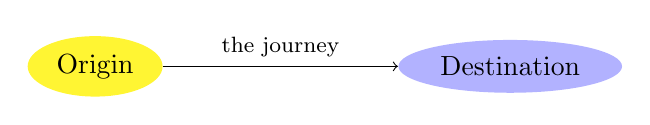
\begin{tikzpicture}
        \node[fill=yellow!80,ellipse] (origin) {Origin};
        \node[fill=blue!30,ellipse] (destination) at (15em,0) {Destination};
        \path (origin) edge[->] node[above,font=\footnotesize] {the journey}
        (destination);
    \end{tikzpicture}
    \caption{TikZ drawings will be output as SVG, which should be rendered by most modern browsers.}
\end{figure}

\begin{figure}[!ht]
    \centering
    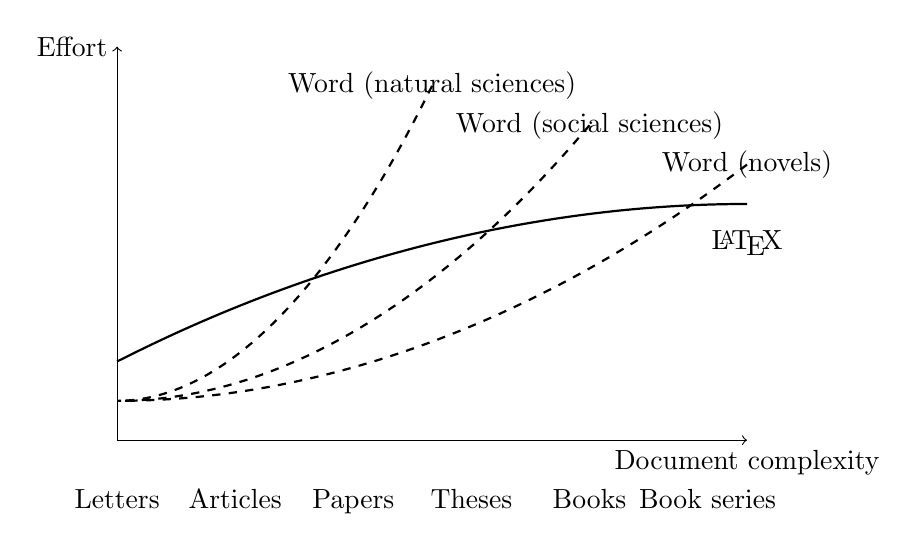
\begin{tikzpicture}

    % horizontal axis
    \draw[->] (0,0) -- (8,0) node[anchor=north] {Document complexity};
    \draw[->] (0,0) -- (0,5) node[anchor=east] {Effort};
    
    % labels
    \draw	(0,-0.5) node[anchor=north] {Letters}
    		(1.5,-0.5) node[anchor=north] {Articles}
    		(3,-0.5) node[anchor=north] {Papers}
    		(4.5,-0.5) node[anchor=north] {Theses}
    		(6,-0.5) node[anchor=north] {Books}
    		(7.5,-0.5) node[anchor=north] {Book series};
    
    \draw (8,3.5) node {Word (novels)};
    \draw (6,4) node {Word (social sciences)};
    \draw (4,4.5) node {Word (natural sciences)};
    \draw (8,2.5) node {\LaTeX{}};
    
    % Psis
    \draw[thick,dashed] (8,3.5) parabola[bend at end] (0,0.5);
    \draw[thick,dashed] (6,4) parabola[bend at end] (0,0.5);
    \draw[thick,dashed] (4,4.5) parabola[bend at end] (0,0.5);
    \draw[thick] (0,1) parabola[bend at end] (8,3);

\end{tikzpicture}
    \caption{Comparing complexity of \textit{Word} and \LaTeX{} depending on the application.}\label{fig:latexeffortcomplexity}
\end{figure}

\begin{figure}[!ht]
    \centering
    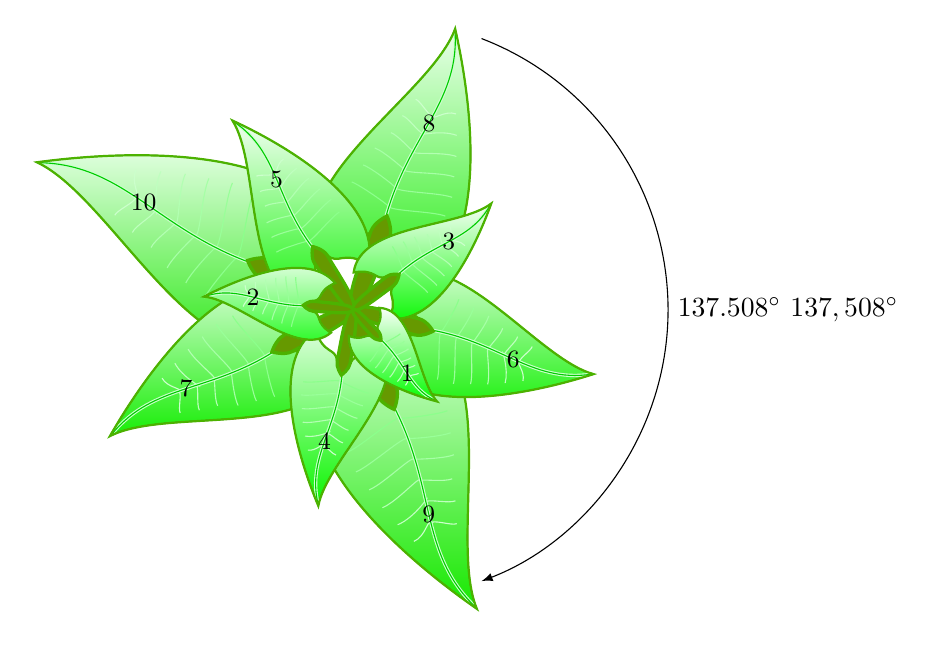
\begin{tikzpicture}
    \foreach \x in {10,...,1}
    {\draw[shade,bottom color=red!\x!green,top color=green!\x,x=0.3 pt,y=0.3 pt,scale={0.4+0.1*\x},rotate=222.5*\x] (0,0) .. 
    controls ( -11,  1) and ( -9, 50) .. (-10,80) ..
    controls ( -16, 60) and (-32, 75) .. (-50,40) .. 
    controls (-110,100) and (-0,230) ..  (  0,300)  node[below] (\x) {} ..
    controls (  45,230) and (110,100) .. ( 50,40) ..
    controls (  32, 75) and ( 16, 60) ..  ( 10,80) ..
    controls (   9, 50) and ( 11,  1) .. (  0,0) 
    -- cycle ;
    
    \draw[thin,green!45,x=0.3 pt,y=0.3 pt,scale={0.4+0.1*\x},rotate=222.5*\x] (-45,120) .. controls (-35,120) and (0,110) .. (-3,110) .. controls (0,105) and (40,120) .. (55,120);
    \draw[thin,green!40,x=0.3 pt,y=0.3 pt,scale={0.4+0.1*\x},rotate=222.5*\x] (-40,140) .. controls (-30,140) and (0,130) .. (-3,130) .. controls (0,125) and (40,140) .. (55,140);
    \draw[thin,green!35,x=0.3 pt,y=0.3 pt,scale={0.4+0.1*\x},rotate=222.5*\x] (-35,160) .. controls (-25,160) and (0,150) .. (0,150) .. controls (0,145) and (35,160) .. (50,160);
    \draw[thin,green!30,x=0.3 pt,y=0.3 pt,scale={0.4+0.1*\x},rotate=222.5*\x] (-25,180) .. controls (-17,180) and (0,170) .. (3,170) .. controls (0,165) and (30,180) .. (45,180);
    \draw[thin,green!25,x=0.3 pt,y=0.3 pt,scale={0.4+0.1*\x},rotate=222.5*\x] (-20,200) .. controls (-13,200) and (0,190) .. (6,190) .. controls (0,185) and (20,200) .. (38,200);
    \draw[thin,green!20,x=0.3 pt,y=0.3 pt,scale={0.4+0.1*\x},rotate=222.5*\x] (-13,220) .. controls (-8,220) and (3,210) .. (8,210) .. controls (10,205) and (18,220) .. (30,220);
    \draw[very thick,green!20,x=0.3 pt,y=0.3 pt,scale={0.4+0.1*\x},rotate=222.5*\x] (0,90) .. controls (-10,180) and (30,230) .. (1,297);
    \draw[thin,black!20!green,x=0.3 pt,y=0.3 pt,scale={0.4+0.1*\x},rotate=222.5*\x] (0,90)  .. controls (-10,180) and (30,230)  .. (1,297) node[midway,black] (num\x) {\small\x};
    \draw[very thick,red!30!green,fill=red!40!green,x=0.3 pt,y=0.3 pt,scale={0.4+0.1*\x},rotate=222.5*\x] 
    (0,0) .. 
    controls ( -11,  1) and ( -9, 50) ..
    (-10,80) .. 
    controls (-10,90) and (0,100) .. (0,100) ..
    controls (0,100) and (10,90) .. (10,80)..
    controls (   9, 50) and ( 11,  1) .. (  0,0) 
    -- cycle;
    \draw[thick,red!30!green,x=0.3 pt,y=0.3 pt,scale={0.4+0.1*\x},rotate=222.5*\x] (0,0) .. 
    controls ( -11,  1) and ( -9, 50) .. (-10,80) ..
    controls ( -16, 60) and (-32, 75) .. (-50,40) .. 
    controls (-110,100) and (-0,230) ..  (  0,300) ..
    controls (  45,230) and (110,100) .. ( 50,40) ..
    controls (  32, 75) and ( 16, 60) ..  ( 10,80) ..
    controls (   9, 50) and ( 11,  1) .. (  0,0) 
    -- cycle ;
    }
    \draw[->,>=latex,x=0.3 pt,y=0.3 pt,black] ([xshift=6pt] 8.east) arc (69:-69:350) node[midway,right] {$137.508^\circ$ $137,508^\circ$};
\end{tikzpicture}

    \caption{Example of a drawing made in TikZ.}\label{fig:leaves-golden-cut}
\end{figure}

\begin{figure}[!ht]
    \centering
    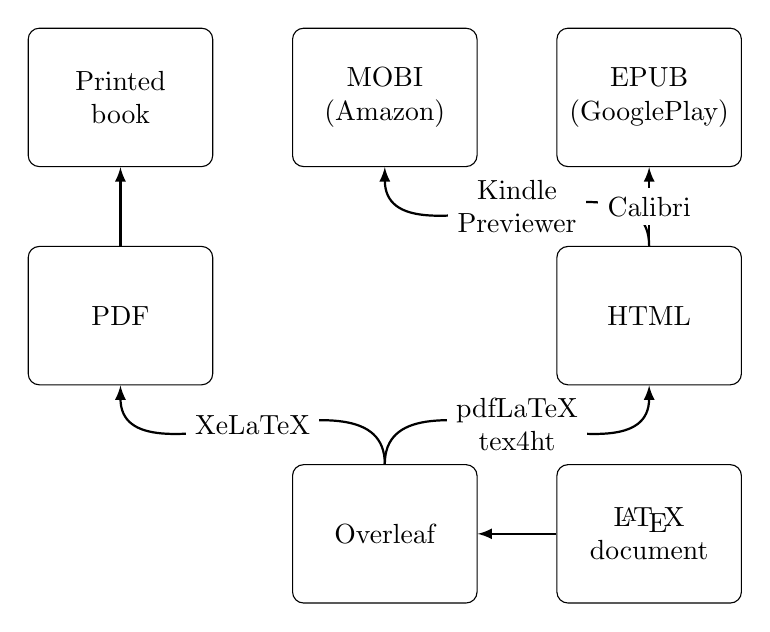
\begin{tikzpicture}
    % Define styles of various tikz elements.
    \tikzstyle{textbox} = [rounded corners, text width=60pt, minimum height=50pt,text centered,draw=black]
    \tikzstyle{arrow} = [thick,->,>=latex]
    \tikzstyle{block} = [rectangle,textbox]
    \tikzstyle{textarr} = [rectangle,align=center,fill=white]

    \node (latex) [block] {\LaTeX{}\\document};
    \node (overleaf) [block, left=of latex] {Overleaf};
    \node (pdf) [block, above left=of overleaf] {PDF}; % xelatex
    \node (html) [block, above right=of overleaf] {HTML}; % pdfLaTeX + tex4ht
    
    \node (print) [block, above= of pdf] {Printed\\book};
    \node (mobi) [block, above left=of html] {MOBI\\(Amazon)}; % Kindle Previewer
    \node (epub) [block, above= of html] {EPUB\\(GooglePlay)}; % Calibri
    
    \draw[out=90,in=270] [arrow] (overleaf) to node[textarr] {XeLaTeX} (pdf);
    \draw[out=90,in=270] [arrow] (overleaf) to node[textarr] {pdfLaTeX\\tex4ht} (html);
    
    \draw [arrow] (latex) -- (overleaf);
    \draw [arrow] (pdf) -- (print);
    
    \draw[out=90,in=270] [arrow] (html) to node[textarr] {Kindle\\Previewer} (mobi);
    \draw [arrow] (html) -- node[textarr] {Calibri} (epub);
\end{tikzpicture}
    \caption{Example 2 of a drawing made in TikZ.}\label{fig:buildchain}
\end{figure}

\chapter{Temporal Side Channels I} 

\section{History}
In 1995, When he was 22, Paul Kaucher released a paper called Timing attacks on implementations of Diffie-Helman, RSA, DSS and other systems \cite{kocher1996timing}.

Before it was published, he wrote about it in a mailing list of Cypherpunks\footnote{A cypherpunk is any activist advocating widespread use of strong cryptography and privacy-enhancing technologies as a route to social and political change. Originally communicating through the Cypherpunks electronic mailing list, informal groups aimed to achieve privacy and security through proactive use of cryptography}
which included all sorts of people like mathematicians, photographers, artists anarchists and more.
The attack was first demonstrated in 1997 in a cryptography conference.
And later, in 1998 an academic paper was published describing how to perform the attack.



\section{The Threat Model}
Figure \ref{c1_fig_threat_model} descirbes the Threat Model on an implementation of some secure system.
It is important to mention that we're talking about attacking an implementation, and not the algorithm itself as we consider the algorithm or protocol being examined as completely secure.

\begin{figure}[H]
    \centering
    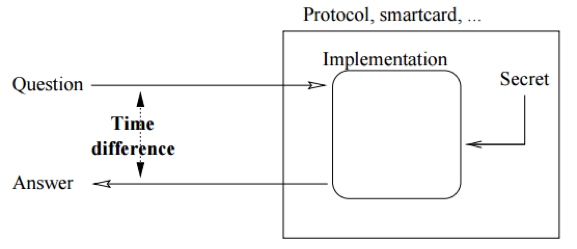
\includegraphics{images/chapter_1/threat_model.png}
    \caption{The Threat Model. Image from JF Dhem1998.
     The attacker can send a message to the implementation and get an answer from it. Also - the attacker is able to measure the time it takes for the implementation to compute the output}
    \label{c1_fig_threat_model}
\end{figure}

\subsection{When is a timing attack even possible?}
\begin{enumerate}
    \item Physical access to the device.
    (for example: Smart card, Crypto wallet, Electronic voting machines)
    \item Sharing a virtual machine with the service
    (for example: Swiping a credit card)
    \item Remote access to a device (access to a device over the network, which may be very noisy and may be rather difficult to implement)
\end{enumerate}

The objective of the attacker to discover the password. And what could the attacker do? The attacker can send unlimited queries and measure their time. Unlimited queries are not so trivial, If you think about it. Some devices can disable themselves after 3 or 4 or 5 periods. This can be a defense \cite{ATM_bruteforce_block}

\section{Timing attack}

\begin{figure}[H]
    \centering
    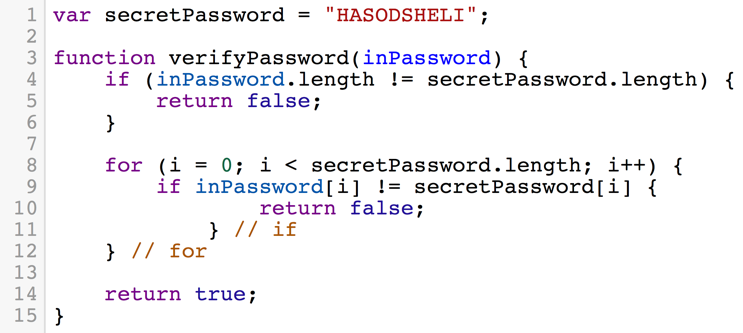
\includegraphics{images/chapter_1/password_check_algo_1.png}
    \caption{A simple and efficient password checking algorithm.
    In line 4 there's a check if there length of the password is the same as the length of the input.
    In line 8 there's an iteration over all of the characters in the }
    \label{c1_fig_pass_check_1}
\end{figure}

Consider the algorithm for password checking as described in figure \ref{c1_fig_pass_check_1}

In a scenario where timing attack is not possible, breaking the password requires the attacker
 to bruteforce the password.
 That is, checking every possible string for one successful attempt.

Let's assume the password is of length 16, if the password only contains english upper-case characters we have 26 possible values for each of the 16 characters in the password.
The first character has 26 possiblites, the second has 26 possiblites and so on. 
So bruteforcing a password like this requries ${26}^{16}$ different attempts, which cannot be completed by any computer in a decent amount of time.
In general, for a password of length $n$ and character range of size $k$,
 breaking the password will take $O({k}^{n})$ attempts.

Now let's consider the scenrio where \textbf{timing attack is possible}. To perform a timing attack,
the attacker takes advantage of the fact that when the program checks for strings equality, the comparison will finish as soon as it finds one character that doesn't match.
Consider the following example where the attacker tries the 3 following attempts and measures
the time it takes for the machine to respond. The attacker tries "AAAA" and measures 0.2ms, then tries "BAAA" and measures 0.5ms lastly tries "CAAA" and measures 0.2ms again.
The attack can be pretty sure that the first character is "B".
Now, checking the whole password does not require iterating of all possible combinations of strings of size $n$. 
All it takes is to iterate over all possible values of each character, say $k$, and repeat that $n$ times.
This results in a total runtime of $k+k+k+\dots = nk = O(n)$

We can now break the password in a reasonable amount of time, even without knowing the 
length of the password we're trying to crack.

\section{Timing Attack Defenses}
After discussing the potential of such attack, we now consider the possible mitigations we can 
implement on our system to prevent such attacks.

\subsection{Mitigation}
We can consider adding a random wait time after checking each one of the characters.
The problem of course is that the whole process of checking a valid process becomes slower.
And of course, if the attacker can perform a lot of measurements on our system, since the noise is random, the attacker would be able to ignore it.


\subsection{Prevention}
The second type of countermeasure is prevention, making sure that our system is completely resistant to timing attacks.

\subsubsection{Prevention Method 1: Padding}
\begin{figure}[H]
    \centering
    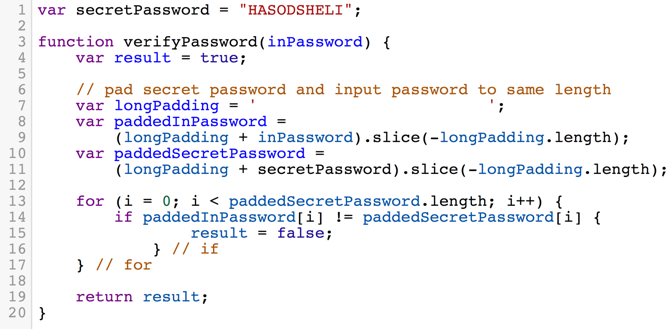
\includegraphics{images/chapter_1/password_check_algo_2.png}
    \caption
    {Prevention method 2, padding the user guess and the secret password to the 
    same length and check all characters even if there's a mismatch in the first character.}
    \label{c1_fig_pass_check_2}
\end{figure}

The first method we examine is to pad the secret password and the user's guess to the same length.
Also - we do not return as soon as we see a character mismatch.
 The code is described in figure 
 \ref{c1_fig_pass_check_2}

The problem with this implementation is that every time there's a character mismatch we execute additional code.
Which is loading the variable \lstinline{result} and writing the value \lstinline{false} to it.
This may seem insignificant in the beginning but actually, this is makes our code \textbf{much more vulnerable than it was before}.
As now the time of it takes for the entire function to complete is linearly dependant on the amount of characters mismatches we have, 
this allows an attacker to perform the same attack from before with no significant changes to his original timing attack.

One might think of a fix which is adding another branch to the \lstinline{if} statement that will do some garbage operation like \lstinline{foo = false}
just so that the attacker might not be able to tell the difference between a match and a mismatch.
The problem with this fix might be that the access time to one variable may be different than the access time to another variable,
and the attacker will be able to tell the difference between them.


\subsection{Prevention Method 2: Hashing}
\begin{figure}[H]
    
    % \centering
    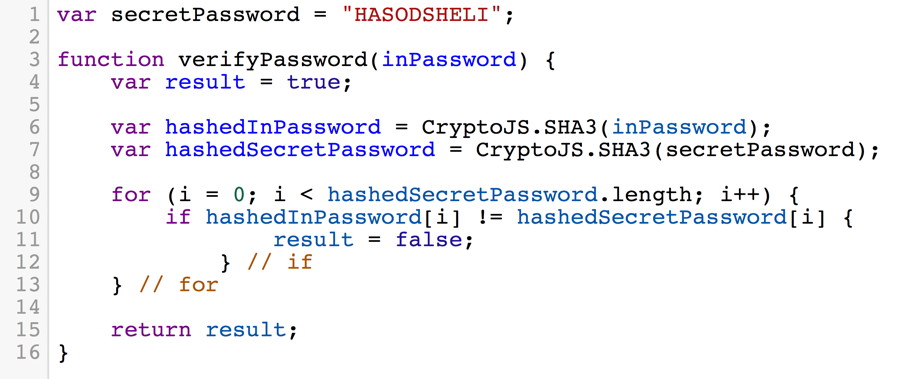
\includegraphics[scale=0.6]{images/chapter_1/password_check_algo_3.png}
    \caption{Secure password checking using a secure hash function}
    \label{c1_fig_pass_check_3}
\end{figure}

The right way to store passwords is with hashing (storing the hash of the password
rather than the password in plain text). A hash is a cryptographic function which has the property called "The Avalanche Property" which means
if even 1 bit is fliped in the input, at least half of the bits of the output are flipped as a result.
This means that even if my guess is really close to the password (1 bit away from the real password) I cannot really know which bits are correct and which are not due to the Avalanche property.

Using hashes to perform a secure password check is described in the algorithm in figure \ref{c1_fig_pass_check_3}
A guess is being hashed before it is compared against the hash of the true password.
An attacker might use the same methods from before to try to leak the hash of the true password, 
 but that would be very difficult as the attacker does not input the hash, the attacker only controls a string that is later being hashed by the algorithm.
 So the trying the methods from before to leak the password would not work if the hash used is propely implemented. 

A possible leak that can occur from this method is the length of the true password.
In line 7 of the algorithm in figure \ref{c1_fig_pass_check_3} the hash of the true password is computed.
Line 7 makes the total run time of the program dependant of the length of the true password.
While this might be risky, this is easy to fix - we can just precompute the hash of the true password
and use it whenever the algorithm runs. This is done for example in Linux where the hashes 
of user's passwords are stored in a file in \lstinline{/etc/shadow}.


\section{The Algebra Behind RSA}
The next thing we're going to perform a timing attack on is the RSA crypto system.
But before we delve into how we break RSA (next chapter) we're going to discuss the
algebraic foundation of RSA \cite{kaliski2006mathematics}.

The RSA cryptosystem lives in something called a multiplicative group.
The group that is $Z^{*}_n$.

We're taking 2 random prime numbers; $p$, $q$ and assign $n=pq$. The group $Z^{*}_n$ 
contains all the numbers from 1 to $n-1$ which do not divide $n$ (that is, do not divide $p$ or $q$).
For example: for $p=3$ and $q=5$, $n= 3*5 = 15$ so $Z^{*}_n = {\{1,2,4,7,8,11,13,14\}}$.

Like all groups, this group has the associative operation which in our case is the modular multiplication,
that is because we mentioned before that this group is a multiplicative group.
The group is also closed under that operation.

The group also has an identity element, 1. Which when multiplied by another element from the group - does not change it.

The last property this group has is that every element $r$ in the group
has an inverse element $r^{-1} \in Z^{*}_n$.

Since the exponentiation is just repeated multiplication - we consider exponentiation 
to also be a closed operation under that group. Each element has an order, the order always divides $(p-1)(q-1)$ (Fermat's little theorem).
When the element is raised to the power of the order, the result of the exponentation (under the modulu of course) is 1, the identity element in the group.

It also important to note that we cannot compute $(p-1)(q-1)$ from knowing $n$

\subsection{Elementary Operations of RSA}
To use the RSA crypto system to encrypt and decrypt messages you first have to generate the infrastructure.
That is deciding on $p$ and $q$ both large prime numbers and computing $n = pq$ and $(p-1)(q-1)$ denoted as $\phi(n)$

\begin{itemize}
    \item \textbf{Choosing a public and private key pairs}
    Choose $e \in Z^{*}_{\phi(n)}$, $d \in Z^{*}_{\phi(n)}$ such that $ed = 1$ mod $\phi(n)$.
    The public key is the pair $\langle{n,e}\rangle$  and the private key pair is  $\langle{n,d}\rangle$.
    \item \textbf{To encrypt a message}
    Choose $m \in Z^{*}_n$ as your message.
    The cipher is $m^{e}$ mod $n$ = $c$
    \item \textbf{To decrypt a message}
    Since $c = m^{e}$ mod $n$, perform $c^{d}$ = $m^{ed}$ = $m^{1}$ = $m$ mod $n$
\end{itemize}

Example: Consider $p = 3$, $q = 5$. So we can compute $n = 3*5 = 15$ and $\phi(15) = 2 * 4 = 8$
Let's assume we choose $e = 3$ and $d=11$. We consider the message 2.

To encrypt, we compute $2^{3} = 8$ mod 11, Which is the cipher. And to decrypt, we're using the private key $11$ as follows: $8^{11}$ = 2 mod 15.
And now we have our message back, 2.

Since this is not a crypto course, we will not go into any much more details about the algebra behind RSA.
However it is important for us to get familiarize with the basics of RSA in order to understand later
how it was optimized and how can we break it.

\subsection{See also}
\begin{enumerate}
    \item John Wiley and Sons Chichester , "Overview about Attacks on Smart Cards by Wolfgang Rankl, Munich", 3rd edition at John Wiley and Sons in September 2003.
    \item Thomas Popp, "An Introduction to Implementation Attacks and Countermeasures", Graz University of Technology, Institute for Applied Information Processing and Communications (IAIK) Graz, Austria.
\end{enumerate}

\chapter{Replace with Third Chapter Name} \label{c3_thirdchapter:cha}

\begin{figure}
    \centering
    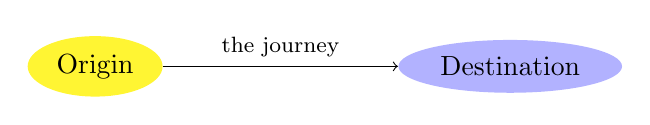
\begin{tikzpicture}
        \node[fill=yellow!80,ellipse] (origin) {Origin};
        \node[fill=blue!30,ellipse] (destination) at (15em,0) {Destination};
        \path (origin) edge[->] node[above,font=\footnotesize] {the journey}
        (destination);
    \end{tikzpicture}
    \caption{TikZ drawings will be output as SVG, which should be rendered by most modern browsers.}
\end{figure}

\begin{figure}
    \centering
    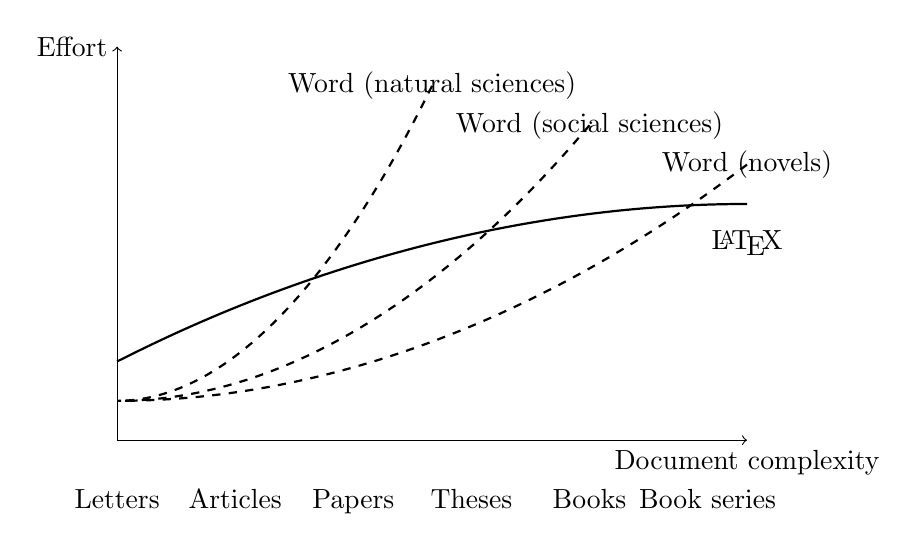
\begin{tikzpicture}

    % horizontal axis
    \draw[->] (0,0) -- (8,0) node[anchor=north] {Document complexity};
    \draw[->] (0,0) -- (0,5) node[anchor=east] {Effort};
    
    % labels
    \draw	(0,-0.5) node[anchor=north] {Letters}
    		(1.5,-0.5) node[anchor=north] {Articles}
    		(3,-0.5) node[anchor=north] {Papers}
    		(4.5,-0.5) node[anchor=north] {Theses}
    		(6,-0.5) node[anchor=north] {Books}
    		(7.5,-0.5) node[anchor=north] {Book series};
    
    \draw (8,3.5) node {Word (novels)};
    \draw (6,4) node {Word (social sciences)};
    \draw (4,4.5) node {Word (natural sciences)};
    \draw (8,2.5) node {\LaTeX{}};
    
    % Psis
    \draw[thick,dashed] (8,3.5) parabola[bend at end] (0,0.5);
    \draw[thick,dashed] (6,4) parabola[bend at end] (0,0.5);
    \draw[thick,dashed] (4,4.5) parabola[bend at end] (0,0.5);
    \draw[thick] (0,1) parabola[bend at end] (8,3);

\end{tikzpicture}
    \caption{Comparing complexity of \textit{Word} and \LaTeX{} depending on the application.}
\end{figure}

\begin{figure}
    \centering
    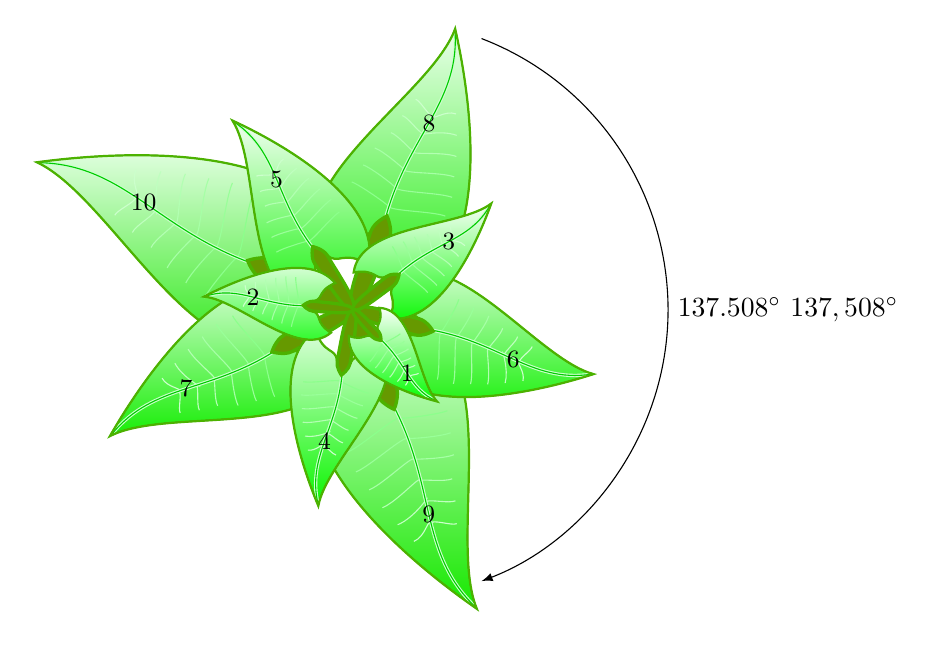
\begin{tikzpicture}
    \foreach \x in {10,...,1}
    {\draw[shade,bottom color=red!\x!green,top color=green!\x,x=0.3 pt,y=0.3 pt,scale={0.4+0.1*\x},rotate=222.5*\x] (0,0) .. 
    controls ( -11,  1) and ( -9, 50) .. (-10,80) ..
    controls ( -16, 60) and (-32, 75) .. (-50,40) .. 
    controls (-110,100) and (-0,230) ..  (  0,300)  node[below] (\x) {} ..
    controls (  45,230) and (110,100) .. ( 50,40) ..
    controls (  32, 75) and ( 16, 60) ..  ( 10,80) ..
    controls (   9, 50) and ( 11,  1) .. (  0,0) 
    -- cycle ;
    
    \draw[thin,green!45,x=0.3 pt,y=0.3 pt,scale={0.4+0.1*\x},rotate=222.5*\x] (-45,120) .. controls (-35,120) and (0,110) .. (-3,110) .. controls (0,105) and (40,120) .. (55,120);
    \draw[thin,green!40,x=0.3 pt,y=0.3 pt,scale={0.4+0.1*\x},rotate=222.5*\x] (-40,140) .. controls (-30,140) and (0,130) .. (-3,130) .. controls (0,125) and (40,140) .. (55,140);
    \draw[thin,green!35,x=0.3 pt,y=0.3 pt,scale={0.4+0.1*\x},rotate=222.5*\x] (-35,160) .. controls (-25,160) and (0,150) .. (0,150) .. controls (0,145) and (35,160) .. (50,160);
    \draw[thin,green!30,x=0.3 pt,y=0.3 pt,scale={0.4+0.1*\x},rotate=222.5*\x] (-25,180) .. controls (-17,180) and (0,170) .. (3,170) .. controls (0,165) and (30,180) .. (45,180);
    \draw[thin,green!25,x=0.3 pt,y=0.3 pt,scale={0.4+0.1*\x},rotate=222.5*\x] (-20,200) .. controls (-13,200) and (0,190) .. (6,190) .. controls (0,185) and (20,200) .. (38,200);
    \draw[thin,green!20,x=0.3 pt,y=0.3 pt,scale={0.4+0.1*\x},rotate=222.5*\x] (-13,220) .. controls (-8,220) and (3,210) .. (8,210) .. controls (10,205) and (18,220) .. (30,220);
    \draw[very thick,green!20,x=0.3 pt,y=0.3 pt,scale={0.4+0.1*\x},rotate=222.5*\x] (0,90) .. controls (-10,180) and (30,230) .. (1,297);
    \draw[thin,black!20!green,x=0.3 pt,y=0.3 pt,scale={0.4+0.1*\x},rotate=222.5*\x] (0,90)  .. controls (-10,180) and (30,230)  .. (1,297) node[midway,black] (num\x) {\small\x};
    \draw[very thick,red!30!green,fill=red!40!green,x=0.3 pt,y=0.3 pt,scale={0.4+0.1*\x},rotate=222.5*\x] 
    (0,0) .. 
    controls ( -11,  1) and ( -9, 50) ..
    (-10,80) .. 
    controls (-10,90) and (0,100) .. (0,100) ..
    controls (0,100) and (10,90) .. (10,80)..
    controls (   9, 50) and ( 11,  1) .. (  0,0) 
    -- cycle;
    \draw[thick,red!30!green,x=0.3 pt,y=0.3 pt,scale={0.4+0.1*\x},rotate=222.5*\x] (0,0) .. 
    controls ( -11,  1) and ( -9, 50) .. (-10,80) ..
    controls ( -16, 60) and (-32, 75) .. (-50,40) .. 
    controls (-110,100) and (-0,230) ..  (  0,300) ..
    controls (  45,230) and (110,100) .. ( 50,40) ..
    controls (  32, 75) and ( 16, 60) ..  ( 10,80) ..
    controls (   9, 50) and ( 11,  1) .. (  0,0) 
    -- cycle ;
    }
    \draw[->,>=latex,x=0.3 pt,y=0.3 pt,black] ([xshift=6pt] 8.east) arc (69:-69:350) node[midway,right] {$137.508^\circ$ $137,508^\circ$};
\end{tikzpicture}


    \caption{Example of a drawing made in TikZ.}
\end{figure}



\chapter{Low Data Complexity Power/EM 2}

We want to see what is power analysis all about and see a very simple power https://www.overleaf.com/project/5d183b17c2fb9f144b44104c analysis attack that we can actually perform. Then we will dive into AES and its implementation.

All the things that we will see today are very optimistic and they assume that we have really good measurements, very good understanding and very good luck, but it's actually quite a little bit harder in practice.

\section{The New York Times, Take 2}
The hero for this article is Mister Kocher. He discovered something that can attack smart cards with what's called power analysis. Probably it was discovered before, but he has discovered it academically.

What did he do? He went to a conference and took people's smart cards and found out their secret private keys. We saw last week that if we have to sign something and we have the private key you can sign a thing that's not supposed to be signed and steal money, this was a big deal.

The 1995 timing attack went to the front page of the New York Times and there was a lot of discussion about the discovery. The 1998 result about power analysis only goes to the bottom of page two in one of the supplements and actually nobody has discussed about it a lot. 

Why didn't he get a lot of attention for this power analysis attack?
Could be because timing is one thing and power analysis is a little more complicated but in the bottom line we can see all the secrets.
To do a timing attack you need a stopwatch, while to power analysis attack you need more sophisticated equipment.

\section{Power Analysis Attacks}
What we need to make timing attack? We just need to be able to send request and gets responses to measured how much it took, while the target can be at the other side of the internet (can Amazon Cloud very far away).

What we need to make Power analysis attack? We need to be physically. 
How do we connect to the device? We need to cut the power supply and connect to it diractly to measure the power consumption.
This is a very invasive attack, we need to be very very close. in 1995 let's assume that it's true. so if we go to the system architect:” listen there is an a power analysis attack that's can completely compromised the device. Attacker needs to come to the device end cuts the power supply….” by the time you already lost the system architect because this is not practical. The threat model has to make sense.
 
nevertheless, the threat model does make sense in a lot of scenarios and we discovered that thing that we was not supposed existing these power analysis and side Channel attack.
today we can attack this device and tomorrow we can attack another device.

To learn about power analysis attack you can go and search in the library the “Power Analysis Attacks” book.
“Cryptanalytic attacks that allow extraction of secret information from cryptographic devices by exploding their power consumption characteristics”
 let's see what can we discover from this definition.
First, What we are attacking here? Cryptographic devices. what we are not attacking? cryptographic algorithms. If I told you that I was able to break RSA on my phone by doing power analysis did I break RSA? No we didn't break RSA, we break the implementation of RSA. 
What else we are not attacking? The user is not under attack, we are not doing any key logging or human engineering attack or social engineering we are only attacking the device.
What's the cryptographic device? Some kind of crypto, signing or encrypting.
What a secret information we wants to extract? Probably we extract the key.
And what's nice about the key? That he has lots of bits. At the start you don't know anything about the key, If you get half of the key you halfway, if you get the whole key You win. If I want to make the device more secure what do I need to do to key? we make a longer key.

This is very easy to say, but if I'm talking instead of secret information we cracked from the device, like medical information, it's a little harder to understand what we can do with half of it. How do we make the medical information more secure? What it's actually means?

Let's take credit cards, the companies say that you are more secure with credit card. Why do we think that we have a privacy with credit cards? We are giving the credit card number and our name... Looks like we're giving everything, the saying that we are actually have privacy, a lot of people have in the US have the same name, but you also get a zip code. Every time you pay with the credit card it generate a new credit card number automatically and doesn't have any digits on him. 
It is very hard to talk about privacy if it's not a cryptographic.
What's left from the definition? we are exploiting the power conceptions characteristic.

What are we not exploiting? We're not doing math and we are not doing something that you can do by algorithms. It's important to know that exploiting the power at conception characteristics does not have to be actually measuring the power. We saw last week that we can actually measure the power consumption with other methods.
When Kotcher wrote his paper he announced three types of power analysis. One of them called Simple power analysis, the other one called differential power analysis. Let's see the simple power analysis today.

\section{Simple Power Analysis}

The simple power analysis means that I'm going to take the measurement of the device, making one measurement or two. With that we are going to get the key from those measurement. What's nice about this attack that it's very reasonable attack model. We need to get the power consumption trace ( this is a vector overtime of the power consumption of the device), and we need only one or two traces. This is actually durable in a lot of scenarios even if I have the device for a little time or even if someone is looking at me. We will see the setup that can be used for simple analysis. 

When you go to a store in Europe, you can't give the credit card for the cashier, they give you this terminale and then you need take your credit card insert it and put the pin number. 
And what is going over here, there is something like a cryptographic computer between your card and terminal. 
Let's assume that we want to attack the card, and it is in my possession. This model is very permissive to me and I can do whatever I want, I can do a lot of transactions I can do radiat, I can twist it and even melt it. so attacking the card is very easy.


But if I don't wants to attack the card? I want to attack the terminal using power analysis. Maybe the terminal has an SSL private key which is used to connect to the Central Center, and this can make a lot of damage and we can be very rich.

We want to do a power analysis on the terminal. This is a nice setup, this is something that looks like a credit card, but it has are wired connected to this fpga and connect to a computer. I will be in a very cold country and I will take this card out from the jacket to my palm. Insert this chip into the terminal, while doing a power analysis on a this terminal. The idea is that I can do it about 1 or two times, but not making it for a thousand times or melt it. I can attack maybe this terminal or a gas station. The fact that we don't need a lot of traces is actually good.

What are the disadvantages? The problem here is that when I look at this power trace I need to be very very well prepared, and understand what's really going on in the power trace. Because we get a vector with a hundred thousand points and we need to understand where is the encryption starting? Where it is ending? What it means that there is a lack of power here a little power there? We need to have a very good understanding of the device processes. 

Not only that we need also to have a very good measurements, because I only have one or two measurements. They're a lot of external Influence on the device, there can be noise, may be related to the device may be related to the environment, and if I have only one measurement I am going to get all of this noise at once and cannot do anything to reduce it. Statistically I'am not going to be able to get clean measurements to perform the attack.

Another problem is that I will need to work very hard to find the key. Let see an example: Yossi did a power analysis measurements and he got a Trace and there was a noise, he did his analysis and got the key. Now he want to check if this is the right key. How can we check the key? Try to decrypt and encrypt the private key. Is this the right key? no it's not :( .. Why? We have only one Trace. Maybe there was noise? Maybe one measurement was wrong? How do we recover from this? We can try a similar key and not there exact key, maybe to change you on bit here or there. This search might be so intensive that we getting basically the same effect like a Brute Force. This makes simple power analysis are not very effective because of all of those reasons.

\section{Other Types of Power Attacks}

So in general in power analysis there are two classes:

\paragraph{Low data complexity attacks} where I get line trace or two traces (a very small amount of traces). Then I do a lot of post-processing and think really really hard and maybe do a reverse engineering before.

\paragraph{High data complexity attacks} I will talk to you about it next week. These attacks require a lot of traces, maybe thousands or Millions traces, a Terabyte of data.

\section{Tuning the power model}

 The first thing that you need to do for a simple power analysis attack is to understand what device you are attacking. We attack two general types of devices with simple power analysis, first is a microcontroller or a CPU and the other thing is ASIC. 
 
Microcontroller is basically a regular computer, it gets commands and runs it one after another, if you want to write a new software for this computer you can write it in C or Java, they're cheap and commonly used.

\begin{figure}[htp]
\hspace*{-0.5in}
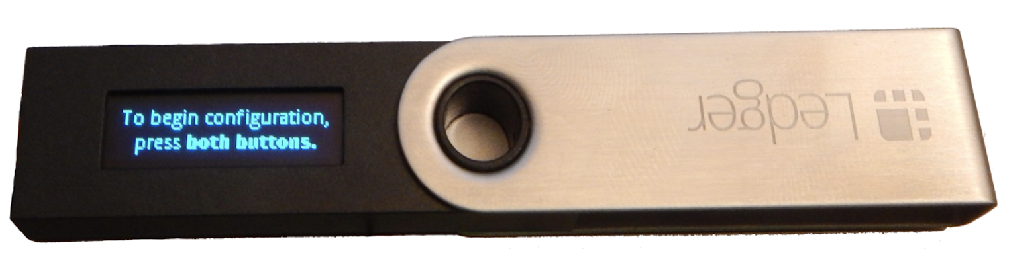
\includegraphics[scale=0.4]{images/Lecture_5/ledger.png}
\caption{Bitcoin Wallet}\label{fig:Bitcoin Wallet}
\end{figure}

This is a Bitcoin wallet. The Bitcoin is basically numbers and if someone steals these numbers he steals your money, so you don't want these numbers to be on your computers. These do all the calculation when you connect to the network, we want it to be very secure because if someone steal the secret key he can take all of your money.

\paragraph{}
Inside this device it has an orange Square and this is the microcontroller. Her some storage and you can write some code for it.

The other kind of a device is called ASIC, this device is manufactured only for a specific purpose. Let's say I want to have a sprinkler that starting the morning and ends in the evening, I will use a programming language that called HDL, once I compiled these software I am not getting an executable program that I can run on a device. These chips can only do one thing, I can't programming them and I can't upgrade them, if there is a bug I am in a big problem, but they have only one purpose. The power consumption of this devices are going to be smaller and sometimes they even be faster. Microcontrollers have programs that runs one line after another, an ASIC can do a parallel operation. ASIC is very cheap to manufacture, but there is a big wrap up before you produced this.

In this course we are going to talk only about microcontrollers, because we are going to see them more often than ASICs. But you will know enough to open the book attacking ASIC.


\begin{figure}[htp]
\hspace*{+0.5in}
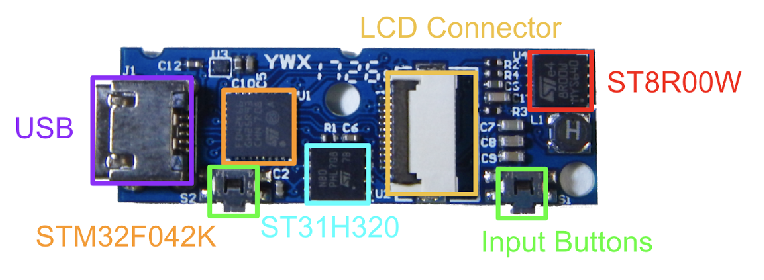
\includegraphics[scale=0.4]{images/Lecture_5/arduino.png}
\caption{Arduino}\label{fig:Arduino}
\end{figure}

So what is the line between microcontroller and an ASIC? On one of the student table there is a chip that he will show us, this is a FPGA field programmable this chip. If I want to identify a particular face I can program this ASIC to do patterning for this face and doing it very very cheaply. I can do also audio compression maybe I don't know what exactly I want to do but I know that I need to do some kind of compression while I don't know exactly the algorithm by using this ASIC. So you will find an ASIC if you have a piece of equipment 10000 pieces, maybe a router ,oscilloscope, submarine and things like that. Best to make sure what is an Arduino? Microcontroller. 


\section{8-bit microcontroller}

This is an 8-bit microcontroller from the 80s, you see the center of this microcontroller , this pair of trousers the red that named ALU, this is where the magic happens, this piece of silicone can actually do logic like multiply, add, shift or compare. 

\begin{figure}[htp]
\hspace*{-0.5in}
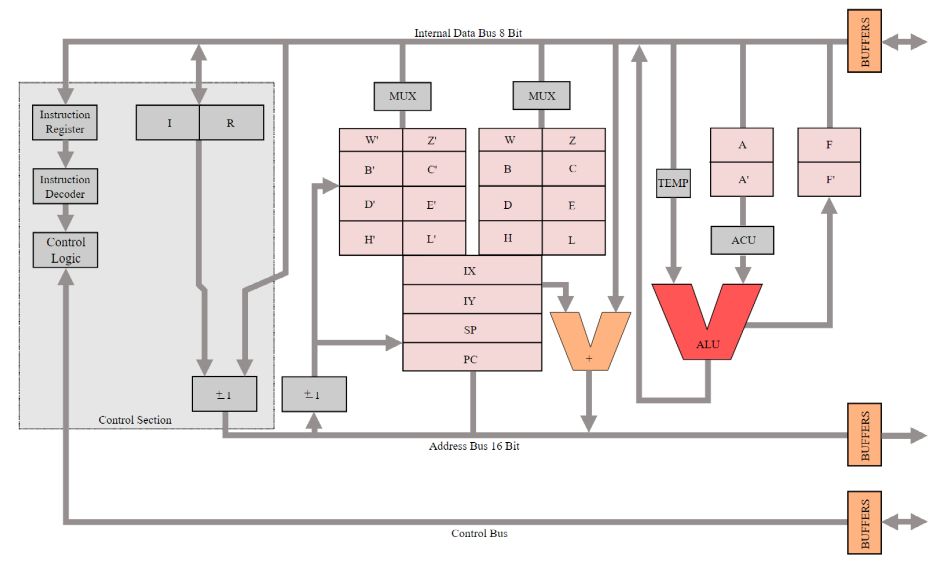
\includegraphics[scale=0.4]{images/Lecture_5/8bit-mc.png}
\caption{8-bit microcontroller}\label{fig:8-bit microcontroller}
\end{figure}


The entire process of life is to get a line of code which represent an instruction, he has to understand what this instruction is trying to do. It can be multiply, read or write. And then you get the operator you need to do from the memory and fed it to the ALU. Then we'll get the next instruction and we'll do it again and again. what's important for me to show you that there is two long in lines from the top and the bottom they are called the buses. the top called the data bus and the bottom call address bus. What is data bus mean? Any sort of data you need to computation has to fetch from this bus. If something come from the memory it going from this bus. If I want to write to external input output, it also going on this bus. The width of this bus is 8 Bits and it means all of the operation that this microcontroller do our eight bits.

On the bottom there is another big bus which is the address bus. If I want to write to memory, I'm going to put their address in the address bus and then I'm going to put the data in the data bus. I will set the control bus to write, and then the memory which is somewhere else is it going to rise to this address. If I want to do a read, I will put the address I want to read in the address bus, and read in the control. What I will do in the data bus? I don't want to put something in there because I want to read, this is actually important and I will elaborate about it more later.

\section{Power Model for Microcontrollers}
What's interesting about microcontroller that there are in many cases the power model don't have Hamming distance and actually have Hamming Weight. What does that mean? That if I think that there are going to be a value going over the bus I don't need to know what was the previous value on the bus, because it's going to be exact humming weight for this value. 

When you have the best that is shared with several components the idea is that all of the components that are not using the bus are going to set how to put them, so all are ones, So if I want for example to read advice from memory the CPU is going to set everything to one and then he is going to extract the memory from the address, then the memory is going to lower all the relevant bits until what sitting on the memory bus and the data bus what I wanted. 

Let's say I want the memory 4, at first I'm going to see on the data bus 0xFF, then I will see 4 and then going to see agaoxin FF because the memory is finished. what was the power-consumption here to go from FF to 4, how many beats has to change? 7, and again it goes back to FF.

\section{Simple Power Analysis of RSA}
Let's see the power module this device under test, which does RSA decryption or signing. While it's doing it we are getting the power measures. Why it is doing an RSA decryption? Because it needs it. We can do it by sending encrypted emails from the phone, so you really have to decrypt the message.

\begin{figure}[htp]
\centering
\hspace*{-0.5in}
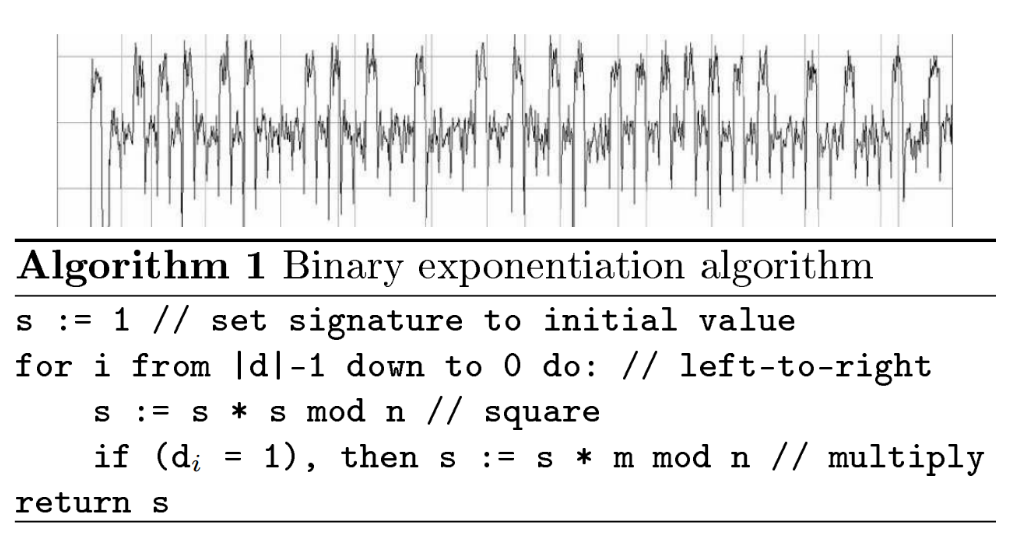
\includegraphics[scale=0.4]{images/Lecture_5/RSA-PA.png}
\caption{RSA Power Analysis}\label{fig:RSA Power Analysis}
\end{figure}

The axis are vector of power measurements, x is time, y are the power consumption,(how did we measure the power consumption? i put a probe, measer the voltege so on..
What is the private key? What is missing? You need to do some reverse engineering first. If this is the only chance to get the key, I need to tell you a little bit more about the device so you will understand what is going on here. This device is microcontroller, it's doing RSA decryption using right to left binary exponentiation using square and multiply. Is it helping you finding the key? Yes. Let me show you the source code.

Binary exponentiation, it starts from the top most bit, off the secret and privates decryption key, and then for each bit we do Square and multiply. If the bit is zero we do Square, if this bit is one we do square and multiply. This help you now finding the key, let's look at that Power Trace.

We see two types of things here, this little thing and the big thing. We have some little thing, big thing, little thing, big thing, and then little little little, and then big thing.

All we need to do is to be able tell about were is the square and were is multiply, and then I can read the key, from top to bottom. So telling about square and the multiply to get to the key is the general method. We see square is take a little power and multiply more power.

What is square? square is multiply. So why is the power consumption of square using multiply is different? this is a microcontroller and his bus width is 8 bit. He's doing a convolution between numbers, so it's multiply thousands of time in frame. so why this is different? So what is consuming power, the ALU is consumer power, the data bus and the address bus consuming power. In this case the power consumption module of the address bus is hemming distance, because it's not setting to 1 between accesses it's always containing what CPU is writing. So did you and multiplication, you are going to see a lot of difference values written into memory to the address bus because this microcontroller have very small component ALU always fetching addresses from memory so ding s*s it's fetching thousands of thousands of memory, but the address is fetching is very similar to each other, because they are all s. les say s is 1k bits in memory all the above are the same but the bathroom are different.But here we are doing s time m, so it's fetching s and m, and you doing convolution. so the address bus when it's doing S and M it’s changing a lot, because he needs to do not only the bottom bits but also the top bits.

\section{Simple Power Analysis of AES}

I am going to attack an 8 bit microcontroller. Let's look on the setup. This microcontroller has a secret key, and it uses an AES encryption. We can ask him to encrypt and decrypt, we send the command in the serial line.

\begin{figure}
\hspace*{0.5in}
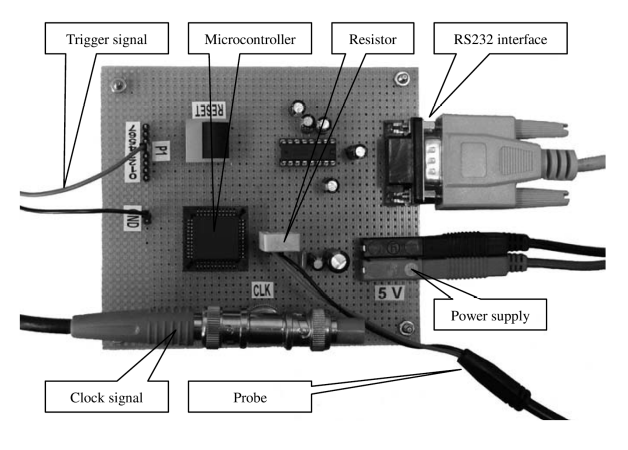
\includegraphics[scale=0.5]{images/Lecture_5/AES_setup.png}
\caption{AES Setup}\label{fig:AES Setup}
\end{figure}
 
While he's doing this operation it is going to consume different amount of power and we would like to measure that. How do we going to measure them? We going to connect to the microcontroller power supply. But were do we need to cut and connect? The power is not going straight to the device it is going from this white box (small resistor). How much power is going to go through the resistor? Because he's small it's going to take very small power consumption. The voltage drops across this device is going to be measured by this Probe, and I'm going to measure the voltage over time. We know the voltage of the power supplies is 5 volt, so from this we can find out what is the current going through the microcontroller and from the current we can find out what is the power consumption. Do we need the code of the microcontroller? Yes. The only thing I don't know is what? The secret, but I know everything else.
 
\section{Advanced Encryption Standard} 
 
What is the story about AES the encryption standard. 

In Death Valley Days encryption was in military standards it was considered like a weapon you weren't supposed to have encryption, not by buy, export or sale. but in the seventies the US government what is it might be a good idea to have civilian encryption to protect civilian identities or health. they went to IBM and ask them to write civilian encryption standard. IBM gave them an algorithm called “Lucifer”, which was based on civilian Knowledge from the World War II, the NSA I analyzed it and they say they don't actually like what you wrote and change it. they changed the key change one of the internal tables and say this was the standard. and the DES actually announced. the changes that NSA made was making it difficult to implement it in software, and to make it Brute Force about using the computing power that has the NSA but to protect it against some kind of attack which was known to the NSA but not known in the Differential cryptography ( not going to teach you).

The time passed and the computer got more and more powerful, there was something called Deep cracking the electronic something, which was able to crack DES at least. I'm not sure if they built it. This was too weak, so introduce something called triple DES, it was twice as secure. Triple DES only used two keys, but we're not going to study in this course. This wasn't so very efficient and it was very slow. The US National standard unit, we want to create a new Cipher which was at least as secure as Triple DES but much more efficient. Efficient on software and hardware and slow computers. Anybody could submit candidates, the winner of this competition was AES, which was a PhD work Raymond and Diamond.

It has some very good properties that we are going to talk about them.

\section{The Advanced Encryption Standard} 

How would you say AES is?, it is an operation which take 2 input, a kye and plain text. And his output is ciphertext. How big is the plain text? 128 bit, The input of the key is not always 16 bits, 16, 64,128 bits. Can go to AES 256 key. No one can break the 256 AES key.
What if I wants to decrypt? AES can be a reverse you can put the ciphertext the key and you get the plain text?. Can we get the plain text and ciphertext so we can get the key? In theory we can do it but the idea is that you cannot get the key. When you feed the key it has to work a little bit, has to extend the key, create around key, this is done in very secure facility.
What if my input is more than 16 bytes? What if I need to encrypt a file? I need to use a protocol and a mode, I can't just use AES, only works on 16 bytes. If I have a larger data I need to use AES with a particular way. Something called AES mode, the famous one called ECB, and CBC, the fashionable called GCM. Not in this course and we don't really care, don't use ECB.
What if we want to encrypt just one byte? we need to do padding, there is a trick and we need to do something.
Let's talk about the design of a AES, it was designed to resist all of source of the attacks, the attacks which were known in the days of DES. And all sorts of attacks which were discovered using the competition. AES was billed to be resistant for those attacks, script analysis attack but no power analysis attack. They are basically expose the cipher if you have enough plaintext and ciphertext.
 
AES won the competition because it was very fast or efficient. You have three optimization goals when you're building a crypto implementation. You wanted to be fast and to be able to encrypt as many bits. Maybe you want to encrypt all the data in the router? You need to be fast and you want it to be power efficient. You don't want to change your battery, and to be cheap so using as little transistors as possible. Take at least area in the Silicon using a smaller cheep. These three goals are conflict with each other, but if you want go hardcore which AES is very very fast, if you want AES be larger. Particular the AES submission the real-time paper head implementation of a s 8 bit 16 and 32 beats microcontroller which be being used till this day. One thing about a s which is very nice is that if you remember the things that people were very very suspicious about this AES that IBM present and a bunch of tables which values that IBM didn't explain and then the NSA came back sage no so use these different values and they also didn't explain why. I know that the NSA did something good and what's nice about AES that he use a single lookup table for all Xbox and this Lucas table is actually derived from mathematical relationship some kind of a multiplication are over algebra field so it's not so hard there. The design is so simple that you not be able to crypto even if you try. 

\section{AES Internals}
AES is an iterated cipher Which means eats has a very bASIC algorithm call drafts and he does them all over and over again, AES has 10 Rounds, if you wants to do it more complicated you as more and more rounds. How does as operated, you begin with 16 bytes and put them in a cyber that's called stage register and then you're on the round operations on these state bytes, every time you operate operations the plaintext gets mixed with the key and every time you do it it gets more and more. When you finish these 10 Rounds senior stage register you have the ciphertext.

If you want to do it in a reverse you put the ciphertext and the stage register and run the operation run after another and you get the plain text.

Each round consists of 4 basic operations, sub bytes, shift rows, mix columns, and add around key.

Every operation was chosen by the creator Rijndael to achieve a different objective. One of the objectives was to confusion, to make the aisle to put not linear a dependent on the input, and I don't think they wanted to do what is diffusion so all the output will depend on the input. We are mixing the plaintext with the key with each one of the operation.

\subsection{SubBytes}
First one of the AES is sub bytes. Let's talk about this while thinking about attacks. 

How do you implement on 8-bit microcontroller? The state is stored in memory so I have 16 bytes of state, you read the first byte of state and the Sbox. Is a table that stored in memory and the size of the table? 2**8. 

So I have this stage registered which is 16 bytes, and the sub box table 256 bytes. A full loop and I took the first byte, first you read it and then I needed to read from the table who is the address that I just read and then I get the value the Sbox, (we know inside the microcontroller) who does right component units the value of the states and the value of the Xbox table, no XOR them, no store that value in the stage register. Bridge from the state go to the table, reading from the sub byte table and xor, and write.This operation is very very leaky.

\begin{figure}[htp]
\centering
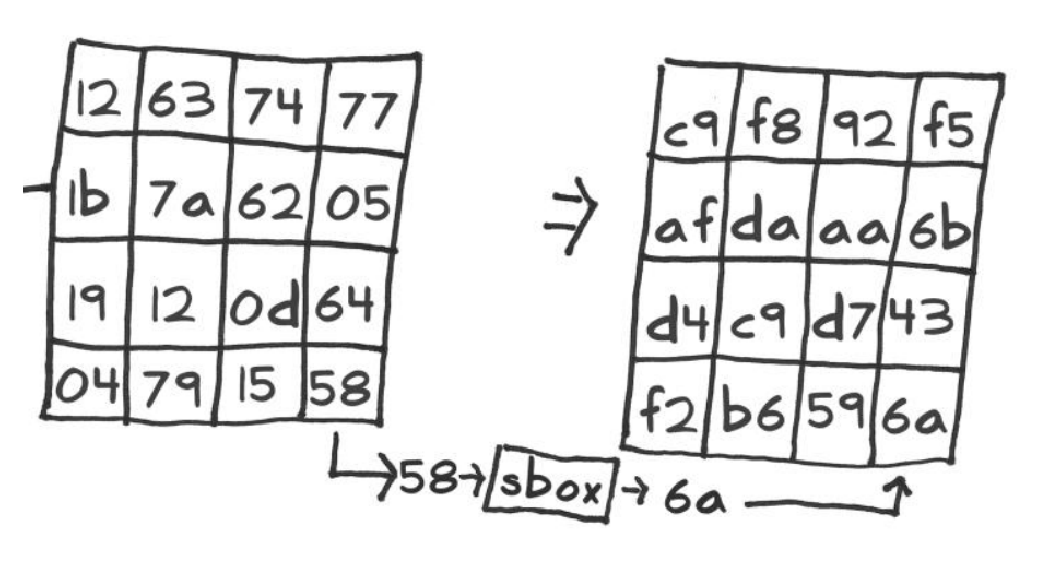
\includegraphics[scale=0.2]{images/Lecture_5/Subbytes.png}
\caption{SubBytes}\label{fig:SubBytes}
\end{figure}

\subsection{ShiftRows}

Then I need to do shift rows. The first row you don't need to do anything, the other rows you need to shift them, how do you shift with 8-bit microcontroller? using a temporary value, I read the state into the temporal value and I'm right it into here. this is also a leaky operation, because I'm leaking all the bytes in the state, well digging the Hemming Weights of the byte. another way to implement it, just by imagination, it doesn't change the data so there are actually operations that don't do shift row.

\begin{figure}[htp]
\centering
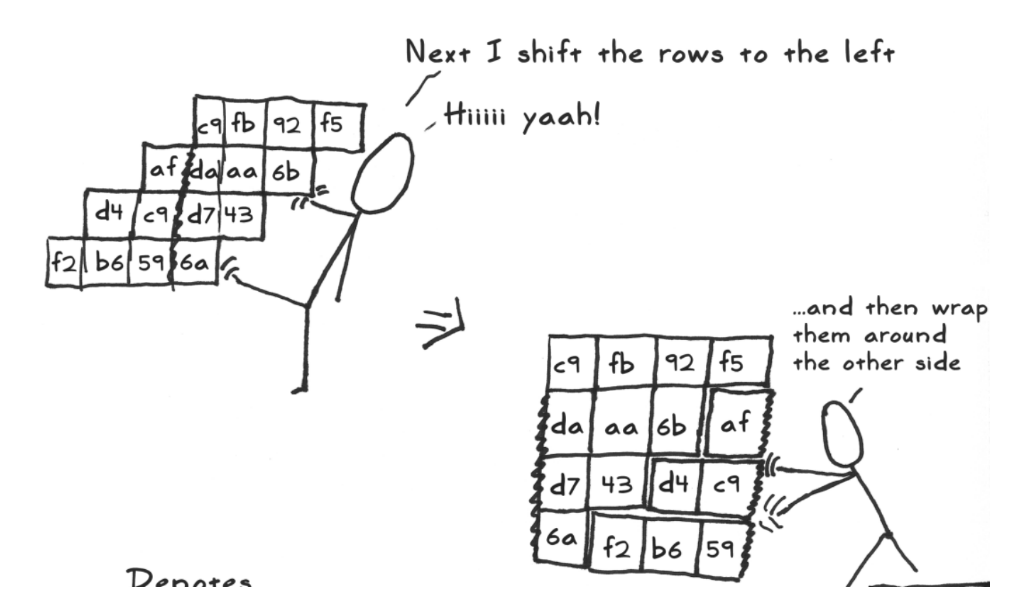
\includegraphics[scale=0.2]{images/Lecture_5/shiftrows.png}
\caption{ShiftRows}\label{fig:ShiftRows}
\end{figure}

\subsection{MixColumns}

Next operation mix columns, is the Matrix a complication, perform over algebra algorithm, it's takes as input 32 bits columns and his output is 32 bytes value what are all of the bytes in the output depend of input. How do you do it on a microcontroller? One of the reasons that rhino run the competition that it was very efficient way was doing mix column 8-bit microcontroller, using 13 operations which are shifts and exor. This is the most leaky part of AES this mixed columns.

\begin{figure}[htp]
\centering
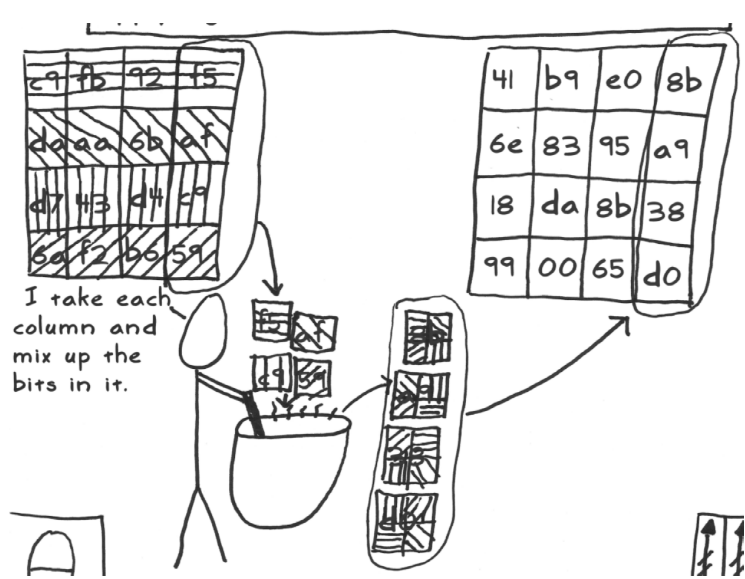
\includegraphics[scale=0.2]{images/Lecture_5/mixcolumns.png}
\caption{MixColumns}\label{fig:MixColumns}
\end{figure}

\subsection{AddRoundKey}

Then do a add round key, just xor, read xor write. This doesn't leak so much because it is inside the ALU, but the reading and writing is the leaking here.
Each round of AES is 84 leaking actions. You take the key and you use the same you used to do in creation but you don't have the plane text yet so you use sub bytes or shift, then you end with the round, and this key expansion is very sensitive for power analysis, you can really attack as very efficiently. We can assume that this expansion is very secure.


\begin{figure}[htp]
\centering
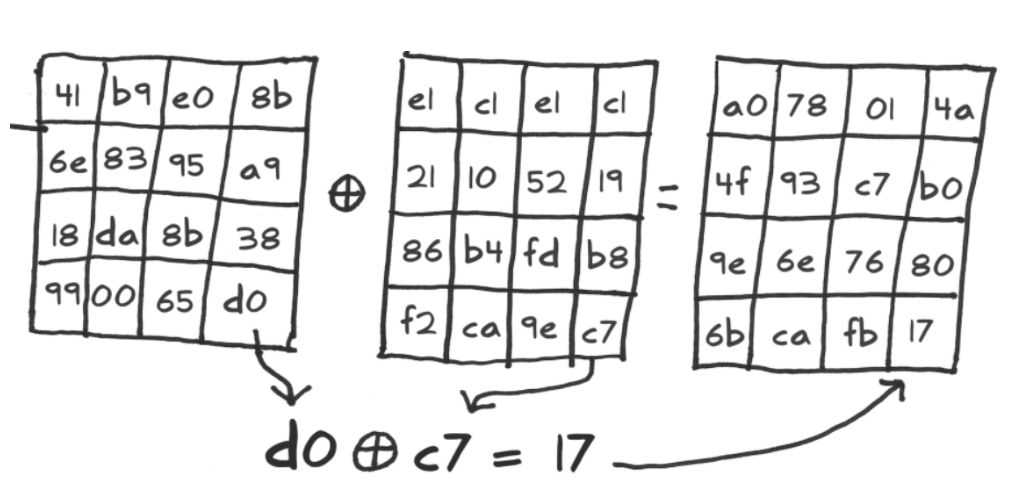
\includegraphics[scale=0.2]{images/Lecture_5/addkey.png}
\caption{AddKey}\label{fig:AddKey}
\end{figure}

\section{AES Power Analysis}
I told you about AES and what is our motivation and what is the structure, and I want to spend the time that has left to show you a little about internal of AES and very very very briefly talk about the reaction of doing simple power analysis of AES. 

\begin{verbatim}
% Make sure the matlab AES scripts are in the path
addpath('matlab_aes_scripts');
%%
% Create two 128-bit plaintexts (exactly 16 byte)
plaintext_1 = uint8('Attack at 12:56!');
plaintext_2 = uint8('Attack at 12:57!');

% how many bits are different between the two?
disp(hamming_weight(bitxor(plaintext_1, plaintext_2)));
%%
% Create a key
key = uint8('1234512345123456');

ENCRYPT = 1;
DECRYPT = 0;
%%
% Encrypt the two plaintexts
ciphertext_1 = aes_crypt_8bit(plaintext_1, key, ENCRYPT); 
ciphertext_2 = aes_crypt_8bit(plaintext_2, key, ENCRYPT);
% even though the plaintexts were very similar...
disp([plaintext_1;plaintext_2]);
% ... the ciphertexts are very different
disp([ciphertext_1;ciphertext_2]);
%%
% how many bits are different between the two?
disp(hamming_weight(bitxor(ciphertext_1, ciphertext_2)));

%%
% Decrypt the two ciphertexts
decrypted_1 =  aes_crypt_8bit(ciphertext_1, key, DECRYPT); 
decrypted_2 =  aes_crypt_8bit(ciphertext_2, key, DECRYPT); 

% Did we get the plaintext again?
disp([plaintext_1;plaintext_2]);
disp([decrypted_1;decrypted_2]);
%%
% Look at the internals of AES now
[ciphertext_1, leak_1] = aes_crypt_8bit_and_leak(plaintext_1, key, ENCRYPT);
[ciphertext_2, leak_2] = aes_crypt_8bit_and_leak(plaintext_2, key, ENCRYPT);

% Show an image showing the two leaks side by size
subplot(1,3,1)
image(squeeze(leak_1));colormap(hsv(256));
subplot(1,3,3)
image(squeeze(leak_2));colormap(hsv(256)); 
figure(gcf)
%%
% Show the difference in the middle
subplot(1,3,2)
image(squeeze(bitxor(leak_1,leak_2)));colormap(hsv(256));
figure(gcf)
%%
% plot the HW of the difference
subplot(1,1,1)
bar(hamming_weight(bitxor(leak_1,leak_2)));
\end{verbatim}

What you see here is Matlab, I wrote this lab environment to do AES implementations, There is code that dose AES, and there i  code that simulates the power leakages of AES as it was implemented on 8-bit microcontroller, all of the operations are 8 bits operations and each time operation happens I'm going to leak it’s Hamming Weight .Let's see what's going on. 

The first thing I'm going to do is to load some libraries and you can find them in the middle, now going to create 216 bytes plain text.
I am going to take these string, to make it binary string Unit8, and I'm going to measure the Hamming distance between these two strings. What is the time distance between these two strings? One, the difference is 6 become 7. 110 - 111.

How do we do it, I have function called bitxor, and this is a vector of size 16,and then waiting Hamming weight. How many possibles Hamming weight are they for 8 bits value? What can the Hamming weight to be? zero,1,2 … 8.So that Hamming weight here is going to be one. 
now I'm going to set up a AES I am going to choose a key.And now I'm going to encrypt AES, and then I'm going to use my to plain text and the key.
The Hamming distance between the two was one. What will be the Hamming distance with the cipher text? Will it be one?no! what's possible values it can be, between 0 to 128, because the output.
Would you like me to be 128? NO, I would like it to be 64. Why do I don't need it to be 100 or 2 or 3. Because that means that I don't have a very important property crypto assistance in the Avalanche property means that each bit in each bit affect all of the input. So if I change one bit in the input and I get only one change in the output it means that I don't have the ability point. But if I change one bit in the input and I get 100 bit change in the output what it is mean? It's means that I don't have the average property and just to make things fun I'm flipping all the bits. What I want the Hamming distance to be is around 64, It's that exactly half of the bits changing.
So you can see I'm doing the Hamming and measuring and show the ciphertext, at the end I'm doing the Hamming weight.
 
These two strings are very very similar until the end, the 6 and 7 change. But if you see the ciphertext you can see a lot of difference. 
And this humming weight is 52. sometimes he's more sometimes is less than 64 but this is okay.
Now let's decrypt, How do I decrypt? I take my AES 8-bit function and I give it decrypt.
The ciphertext and the key. and see if the plain text into ciphertext are the same.
We can see that there are the same and so far so good.
Now I want to show you the internal structure of AES. to do that I have a function that's called 8-bit and leak. Let's open the function.
Here is the function. Let's go over the structure

\begin{verbatim}
function [result state rkeys mixcolumn_leak]= 
aes_crypt_8bit_and_leak(input_data, secret_key, encrypt)

% performs AES-128 encryptions or decryptions like an 8-bit uC would do them
% and leaks internal state 
%
% DESCRIPTION:
%
% [result state rkeys mixcolumn_leak] = aes_crypt(input_data, secret_key, encrypt)
%
% This function performs an AES-128 encryption or decryption of the input
% data with the given secret key.
%
% PARAMETERS:
%
% - input_data:
%   A matrix of bytes, where each line consists of a 16 bytes (128 bit)
%   data input value of the AES-128 en/decryption.
% - secret_key:
%   A vector of 16 bytes that represents the secret key.
% - encrypt:
%   Paramter indicating whether an encryption or a decryption is performed
%   (1=encryption, 0=decryption).
%
% RETURNVALUES:
%
% - result:
%   A matrix of bytes of the same size as the byte matrix 'input_data'.
%   Each line of this matrix consists of 16 bytes that represent the
%   128-bit output of an AES-128 en/decryption of the corresponding line of
%   'input_data'.
% - state:
%   A matrix of byte of size |'input_data'| x 41, containins the state
%   progression of the encryption process.  
%   Legend of the state progression:
%   (P= plaintext, C=Ciphertext, K=after AddKey, B=after SubBytes, R=after
%   ShiftRows, M=after MixColumns)
%   P K BRMK BRMK BRMK BRMK BRMK BRMK BRMK BRMK BRMK BRK(=C)
% - mixcolumn_leak:
%   A matrix of size |'input_data'| x 9 x 4 x 9 (for encryption), or
%                    |'input_data'| x 9 x 4 x 18 (for decryption),
%       where mixcolumn_leak(line, subround, col, :) is the list of
%       intermediate valutes generated by the 8-bit MC operation on the
%       [col] columns of line [line] in the input data during
%       subroun [subround]
% EXAMPLE:
%
% result = aes_crypt([1:16; 17:32], 1:16, 1)


% AUTHORS: Stefan Mangard, Mario Kirschbaum, Yossi Oren
%
% CREATION_DATE: 31 July 2001
% LAST_REVISION: 28 October 2008

state = zeros([41 size(input_data)], 'uint8');
rkeys = zeros([10 16], 'uint8');
if (encrypt == 0) % decryption
    mixcolumn_leak = zeros([9 4 size(input_data,1) 18]);
else % encryption
    mixcolumn_leak = zeros([9 4 size(input_data,1) 9]);
end

for round = 1:10
    rkeys(round,:) = aes_round_key(secret_key,round);
end

% expand the keys

if encrypt == 0 %decryption
    state(41,:) = input_data;

    for i=10:-1:1
        if i ~= 10
            input_data = aes_add_round_key( aes_round_key(secret_key,i), input_data);
            state(3 + (i-1)*4 + 2,:) = input_data;

            [input_data leak] = aes_mix_columns_8bit_and_leak(input_data,0);
            mixcolumn_leak(i, :, :, :) = leak;
            state(3 + (i-1)*4 + 1,:) = input_data;
        else
            input_data = aes_add_round_key( aes_round_key(secret_key,i), input_data);
            state(3 + (i-1)*4 + 1,:) = input_data;
        end

        input_data = aes_shift_rows(input_data,0);
        state(3 + (i-1)*4,:) = input_data;

        input_data = uint8(aes_sbox(input_data,0));
        state(3 + (i-1)*4 - 1,:) = input_data;
    end

    input_data = aes_add_round_key(secret_key, input_data);
    state(1,:) = input_data;

else % encryption

    state(1,:) = input_data;
    input_data = aes_add_round_key(secret_key, input_data);
    state(2,:) = input_data;
    
    for i=1:10
        input_data = uint8(aes_sbox(input_data,1));
        state(3 + (i-1)*4,:) = input_data;

        input_data = aes_shift_rows(input_data,1);
        state(3 + (i-1)*4 + 1,:) = input_data;

        if i ~= 10
            [input_data leak] = aes_mix_columns_8bit_and_leak(input_data,1);
            mixcolumn_leak(i, :, :, :) = leak;
            state(3 + (i-1)*4 + 2,:) = input_data;

            input_data = aes_add_round_key( aes_round_key(secret_key,i), input_data);
            state(3 + (i-1)*4 + 3,:) = input_data;
        else
            input_data = aes_add_round_key( aes_round_key(secret_key,i), input_data);
            state(3 + (i-1)*4 + 2,:) = input_data;
        end
    end
            
end

result = input_data;

\end{verbatim}

First of all I expand the key, so I do the AES key expansion and I don't leak the key expansion. This is the assumption. Let's disregarded that description for a moment and this is the encryption. First of all I took the state and the input data in the state, and then I do a add round key, then do SUB bytes, shift rows, mix column. In the last round I done did you mixed columns, and every time I do this I don't replace the state and I saved the state. at the end I output the cipher text, but also the output to the state, so you can see the state is always changing. Now let's see how does it looks, I'm going to run AES twice, and then do some little figure.

\begin{figure}[!ht]
\centering
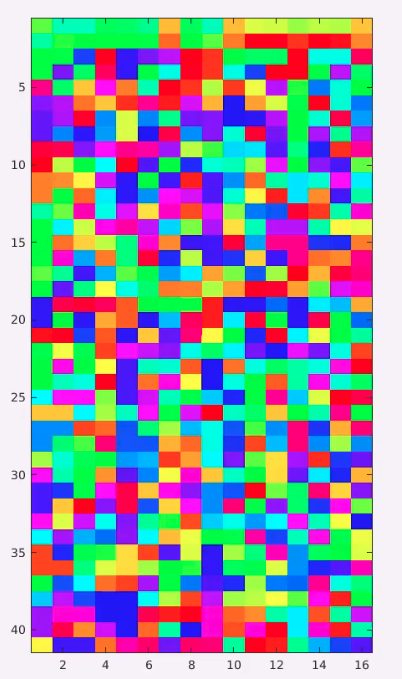
\includegraphics[scale=0.35]{images/Lecture_5/aes_mat_out.png}
\caption{Diagram}\label{fig:Diagram}
\end{figure}

The x-axis is the index of the byte in the state. I read the bytes not as a matrix I read it as a row. So there are 16 bites in the state. and the y-axis is the index of the rounds and round 40 is the final round ciphertext. So in between there is the stages.
You can see that in the beginning it is very very similar.

If you go down it's become much different and in the bottom it's completely different. This is very easy to analyze. And what we are going to do now show the difference between state. What do you see in the middle is the Hemming distance between the right and the left where red is is 0 and blue is 256.

In stage 0 what is the difference between two plain texts? 1 bit, you can see one beat is changed to O. The first round is a add key, we xor the 15 bytes of the key who is 16 bytes of the state, the key is the same in both sides, if the Hamming distance between the two sides was one before I sold the key what is it going to be after? 1. The differential doesn't change at all, I think a distance of 1 and Ikes or a constant of both sides and The Outpost is still the same. so in the first row I can't see differences. look wild sheep will do, one by the interstate here, one byte is in the same place and one byte There and one byte here. Now there are 4 bytes different between the states, but this bytes are all of the column.What is the next operation? mixed columns. See what's mix column did, mixed this change and now all of the bytes of the states are different.We can't stop AES after 2 rounds, it still can break with crypto analysis, but you can see that this is very nice.
 
I want to plug the Hamming weight of the distance, The x-axis here he's there around, and the y-axis is the Hamming distance between the two stay. you can see state with the one then one stays one, after sub byte becomes 4, Shift columns doesn't change the 4, then mix columns make it grow a little bit. And then you see the distance stays around 64 until the end of the encryption.
I want to show you how do we attack AES using simple power analysis.

There is a lot to talk about in very little time. in very very briefly I will give you the ideal way did you it and then I'll show you how it's actually done.
I have connected a probe to my device, I have measured the power consumption overtime. so now I have a vector of size that lets say a hundred thousand, and I know that AES is there. Now I want to find the key out of my measurements from my trace.

\begin{figure}[htp]
\centering
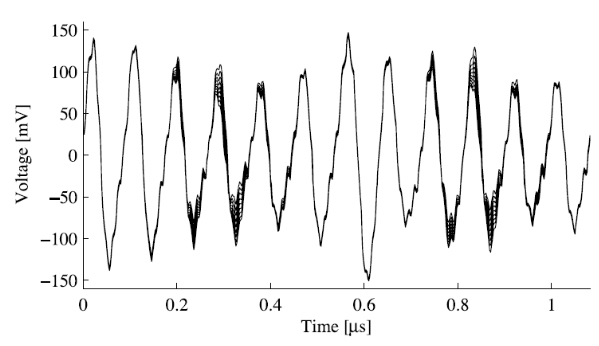
\includegraphics[scale=0.30]{images/Lecture_5/trace1.png}
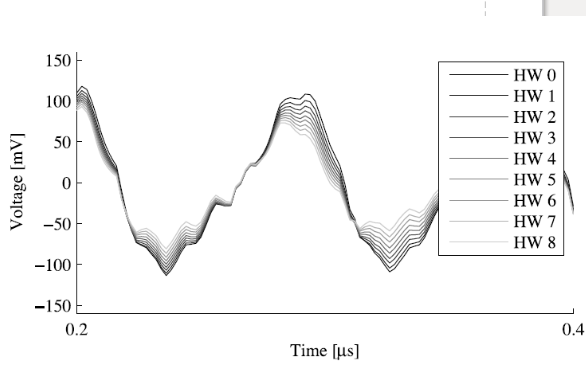
\includegraphics[scale=0.30]{images/Lecture_5/trace2.png}
\caption{Traces}\label{fig:traces}
\end{figure}

I have a trace, which was recorded in the same device we saw here. I have a vector called 200 of traces of AES encryption, lets plot one of the traces. this is actually only one of the rounds of AES. Here is a trace. This is very very clean trace and I would like it to be in my lab.You can see some of them are high and some of them are low, how do I find the key out of this? let's start from the beginning then jump to the middle and the end I don't have time to teach you. the best thing I can hope for is not to get the bytes of the key because the bytes are not function of the bytes, what is the function of? The Hamming weight. So the best hope is the get the Hamming weight, so are you home we will get a vector like the state vector. is this enough to get the key? so you have to believe me that's yes. how do you do it? You will use algebraic the solver and you will have to read the paper. if you have the vector off all the time in Hamming weight you can get the key. But how do I get the vector Hamming weight from distance? Obviously somewhere in this trace, let's look at very very leaky operation like sub bytes, or add around key; it read the states you leave the key and xor them together and then you write the state again. Somewhere in this vector there is a peak where we know that exactly in this moment there was a read of the key. The key was read from memory and was travel in the data bus in this exact peak. And how do I find this particular moment in time I will show you in the next lecture.

So I need to write a function that gets an input about 20 points and what is its out puts? the Hamming weight. maybe it will output of Hamming weight. how do I do it? we need to write a decoder that's as single processing.

Here is a figure showing the move operation they did the same move operation in the microcontroller over and over again this is the average of thousands of measurements where are they moving 0 or 1, until moving 255 ff. Can anybody, you see how Hamming Weight zero have big change, why Hamming weight 0 is more power consumption of Hamming weight 8? Between moves it settings old ones, so moving to zero take more effort from changing.
 
Here is like a longer trace, let's assume I hate this data how do I build the decoder. I want the function that can take an array of values and output Hamming weight. 
Let's start simple, what if I had just one point? I have an input and function that gets one point and give me the Hamming weight of this point. I can calculate the mean each one, the mean for 0 the mean for 1, for 2. if I get it right what we will do, so do you like a nearest neighbor. if I know that the mean of 4 Hamming weight for is 7 and the mean of Hamming weight five is 8 and I got 7.9, what am I going to chose 4 or 5? 5.nearest neighbor.

This is a nice idea, but I have to give them a little extra dangerous. the problem is here that's the Hamming weight are not identically distributed. how many possible values of bytes I get? 256. how many bytes are there with Hamming weight zero? 1. how many bytes Hamming weight 8? 1. how many Hamming weight 1? 8. Hamming weight of 1 is 8 times more likely than Hamming weight of 0. So why do we need to do?we need to do Bayes. The idea is are you going to favor the output more likely. I will found out what are the odds that its five, 6?, 7? then look on my decoder and then I'm going to look and give a bonus for more common Hamming weight. The idea is I need to learn How likely bytes based on the trace decoding and then I'm going to go and look at the distribution of this and then multiply The probability I got. this is for one point. I calculated the odds and then I multiply the probability. what if I have more than one point? watch we actually wants to do here he's actually called multivariate normal distribution. each one of these points, let's say four points, the dimension, and I have a like a cloud In this distribution space, how do you do this? that is the very very fundamental paper called “template power analysis attack” which explain this.

So if you want to do a simple power analysis on AES the steps you do first of all you profiled the device, you understand where all this stuff is happening, you need to build Template that will help you to recognize different Hamming Weight, then you're play the same place in the trace and you get guesses for Hamming weight for each States and you hope you get the right guesses, and then you take this Hamming weight and you take a few equation solver we'll take the Hamming weight and output the key, or something that we don't know? I don't know because noise. If we can correlate the Hamming weight to wrong then the equation solver will fail. what can we do in this case? We try again.

\newpage
\section{Template Attacks} 
\subsection{Introduction}
    Devices performing cryptographic operations can be analyzed by various means.
    Traditional cryptanalysis looks at the relations between input and output data and the used keys. However, even if the implemented algorithms are secure from a cryptanalysis point of view, side-channel attacks pose a serious threat. Sidechannel attacks are a subgroup of implementation attacks. Examples thereof are timing attacks, power attacks like DPA or SPA.
    Traditional DPA style attacks assume the following threat model:
    The secret key stored in the device is used to perform some cryptographic operations. The attacker monitors these operations using captured side-channel information like power consumption or electromagnetic emanation. The attack is successful if the used secret key can be reconstructed after a certain number of operations.\textbf{If the number of operations is limited by the protocol used to initiate} these operations, the attacker has an upper bound on the number of operations he can observe. If the operation, which leaks usable side-channel information, is executed just once, the threat model is different: The attacker has to reconstruct the secret
    key using a single trace of side-channel information. Besides protocol limitations, ephemeral keys can be the reason for such a constraint. Techniques like SPA are a general way to tackle this problem. These techniques useeasily distinguishable features of operations like double and add, or add and multiply, to infer key-bits. The majority of the available literature deals with these two types of scenarios. \textbf{If the observed signal-to-noise ratio is not high enough, or the implementation is done in a way that ensures the used operations being independent of the key(i. e. no key-dependent jumps), SPA style attacks are not possible anymore.} The attacker has to think of other ways to get hold of the secret key: One way to do this is to use a similar device and build a model of it. Using this
    model, an attacker might now be able to recover the secret key.
    
\subsection{Algorithm}
    Template attacks are a powerful type of side-channel attack. These attacks are a subset of profiling attacks, where an attacker creates a ``profile" of a sensitive device and applies this profile to quickly find a victim's secret key.
    
    Template attacks require more setup than CPA attacks. To perform a template attack, the attacker must have access to another copy of the protected device that they can fully control. Then, they must perform a great deal of pre-processing to create the template - in practice, this may take dozens of thousands of power traces. However, the advantages are that template attacks require a very small number of traces from the victim to complete the attack. With enough pre-processing, \textbf{the key may be able to be recovered from just a single trace} .
    
    
    There are four steps to a template attack:
    \begin{itemize}
      \item Using a copy of the protected device, record a large number of power traces using many different inputs (plaintexts and keys). Ensure that enough traces are recorded to give us information about each subkey value.
      \item Create a template of the device's operation. This template notes a few ``points of interest" in the power traces and a multivariate distribution of the power traces at each point.
      \item the victim device, record a small number of power traces. Use multiple plaintexts. (We have no control over the secret key, which is fixed.)
      \item Apply the template to the attack traces. For each subkey, track which value is most likely to be the correct subkey. Continue until the key has been recovered.
    \end{itemize}
    
    \subsection{Signals, Noise, and Statistics}
    Before looking at the details of the template attack, it is important to understand the statistics concepts that are involved. A template is effectively a multivariate distribution that describes several key samples in the power traces. This section will describe what a multivariate distribution is and how it can be used in this context.
    Noise Distributions\\
    Electrical signals are inherently noisy. Any time we take a voltage measurement, we don't expect to see a perfect, constant level. For example, if we attached a multi-meter to a 5 V source and took 4 measurements, we might expect to see a data set like (4.95, 5.01, 5.06, 4.98). One way of modelling this voltage source is: 
    $\mathbf{X} = \mathbf{X} + \mathbf{N}$
    where $\mathbf{X}$
    is the noise-free level and $\mathbf{N}$ is the additional noise. In our example, $\mathbf{X}$ would be exactly 5 V. Then, N is a random variable: every time we take a measurement, we can expect to see a different value. Note that $\mathbf{X}$ and $\mathbf{N}$ are bolded to show that they are random variables.
    A simple model for these random variables uses a Gaussian distribution (read: a bell curve). The probability density function (PDF) of a Gaussian distribution is
    f(x) = $ \frac{1}{\sigma \sqrt{2\pi}} e^{-(x - \mu)^2 / 2\sigma^2}$
    where $\displaystyle \mu$  is the mean and  $ \sigma$ is the standard deviation. For instance, our voltage source might have a mean of 5 and a standard deviation of 0.5, making the PDF look like:\\
    \begin{minipage}{\linewidth}
    \centering
    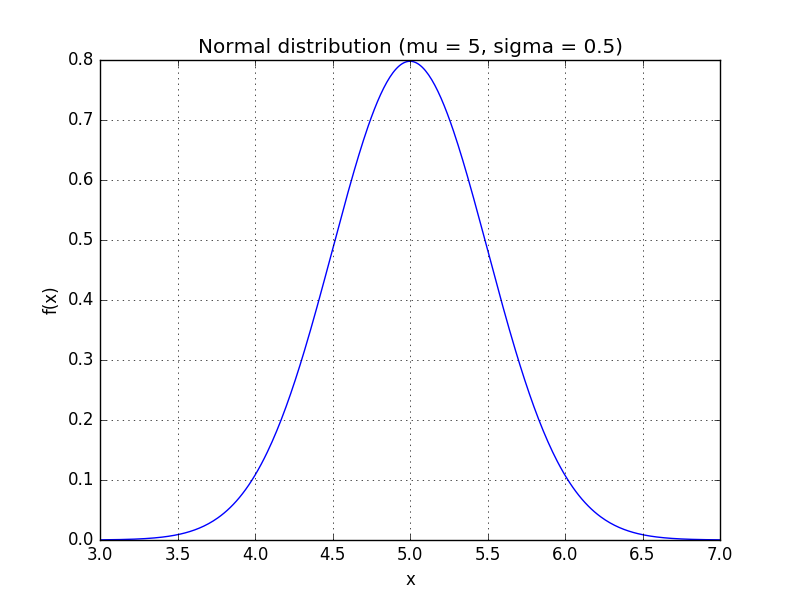
\includegraphics[width=8cm]{images/Lecture_5/Normal-Dist.png}
    \end{minipage}
    We can use the PDF to calculate how likely a certain measurement is. Using this distribution,
    $f(5.1) \approx 0.7821$
    $f(7.0) \approx 0.0003$
    so we're very unlikely to see a reading of 7 V. We'll use this to our advantage in this attack: if f(x) is very small for one of our subkey guesses, it's probably a wrong guess.\\
    Multivariate Statistics
    The 1-variable Gaussian distribution works well for one measurement. What if we're working with more than one random variable?
    Suppose we're measuring two voltages that have some amount of noise on them. We'll call them $\mathbf{X}$ and $\mathbf{Y}$. As a first attempt, we could write down a model for $\mathbf{X}$ using a normal distribution and a separate model for $\mathbf{Y}$ using a different distribution. However, this might not always make sense. If we write two separate distributions, what we're saying is that the two variables are independent: when $\mathbf{X}$ goes up, there's no guarantee that $\mathbf{Y}$ will follow it.
    Multivariate distributions let us model multiple random variables that may or may not be correlated. In a multivariate distribution, instead of writing down a single variance $\sigma$, we keep track of a whole matrix of covariances. For example, to model three random variables ($\mathbf{X}, \mathbf{Y}, \mathbf{Z}$), this matrix would be\\
    \begin{minipage}{\linewidth}
      \centering
      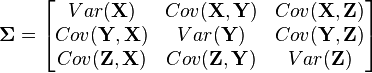
\includegraphics{images/Lecture_5/cov.png}
      \end{minipage}
    Also, note that this distribution needs to have a mean for each random variable:\\
       \begin{minipage}{\linewidth}
      \centering
      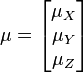
\includegraphics{images/Lecture_5/mu.png}
      \end{minipage}
    The PDF of this distribution is more complicated: The equation for k random variables is:\\
     \begin{minipage}{\linewidth}
      \centering
      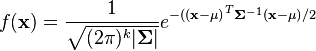
\includegraphics{images/Lecture_5/dist.png}
      \end{minipage}

\subsection{Creating the Template}
    A template is a set of probability distributions that describe what the power traces look like for many different keys. Effectively, a template says: ``If you're going to use key k, your power trace will look like the distribution $f_k(\mathbf{x})$"\\
    . We can use this information to find subtle differences between power traces and to make very good key guesses for a single power trace.\\
    \\
    \textbf{Number of Traces}\\
    One of the downsides of template attacks is that they require a great number of traces to be preprocessed before the attack can begin. This is mainly for statistical reasons. In order to come up with a good distribution to model the power traces for every key, we need a large number of traces for every key. For example, if we're going to attack a single subkey of AES-128, then we need to create 256 power consumption models (one for every number from 0 to 255). In order to get enough data to make good models, we need tens of thousands of traces.
    
    Note that we don't have to model every single key. One good alternative is to model a sensitive part of the algorithm, like the substitution box in AES. We can get away with a much smaller number of traces here; if we make a model for every possible Hamming weight, then we would end up with 9 models, which is an order of magnitude smaller. However, then we can't recover the key from a single attack trace - we need more information to recover the secret key.\\
    \\
    \textbf{Points of Interest}\\
    Our goal is to create a multivariate probability describing the power traces for every possible key. If we modeled the entire power trace this way (with, say, 3000 samples), then we would need a 3000-dimension distribution. This is insane, so we'll find an alternative.
    
    Thankfully, not every point on the power trace is important to us. There are two main reasons for this:
    \begin{itemize}
      \item We might be taking more than one sample per clock cycle.  There's no real reason to use all of these samples - we can get just as much information from a single sample at the right time.
      \item Our choice of key doesn't affect the entire power trace. It's likely that the subkeys only influence the power consumption at a few critical times. If we can pick these important times, then we can ignore most of the samples. 
    \end{itemize}
    
    These two points mean that we can usually live with a handful (3-5) of points of interest. If we can pick out good points and write down a model using these samples, then we can use a 3D or 5D distribution - a great improvement over the original 3000D model.
   \subsection{Analyzing the Data}
    Suppose that we've picked I points of interest, which are at samples $s_i (0 \le i < I)$. Then, our goal is to find a mean and covariance matrix for every operation (every choice of subkey or intermediate Hamming weight). Let's say that there are K of these operations (maybe 256 subkeys or 9 possible Hamming weights).
    
    For now, we'll look at a single operation k $(0 \le k < K)$. The steps are:
    \begin{itemize}
      \item Find every power trace t that falls under the category of ``operation k". (ex: find every power trace where we used a subkey of 0x01.) We'll say that there are $T_k$ of these, so $t_{j, s_i}$ means the value at trace j and POI i.
      \item Find the average power $\mu_i$ at every point of interest. This calculation will look like:
      \begin{figure}[htp]
      \centering
      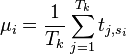
\includegraphics{images/Lecture_5/pc1.png}
      \end{figure}
       
      \item Find the variance $v_i$ of the power at each point of interest. One way of calculating this is:
      \begin{figure}[htp]
      \centering
      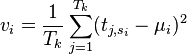
\includegraphics{images/Lecture_5/pic2.png}
      \end{figure}
    
      \item Find the covariance $c_{i, i^*}$ between the power at every pair of POIs $(i and i^*)$. One way of calculating this is:
      \begin{figure}[htp]
      \centering
      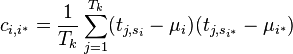
\includegraphics{images/Lecture_5/pic3.png}
      \end{figure}
      \item Put together the mean and covariance matrices as:
    
      \begin{minipage}{\linewidth}
      \centering
      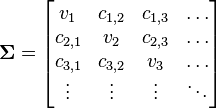
\includegraphics{images/Lecture_5/pic5.png}
      \end{minipage}
      \begin{minipage}{\linewidth}
      \centering
      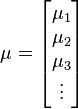
\includegraphics{images/Lecture_5/pic4.png}
      \end{minipage}
      
    \end{itemize}
    
    These steps must be done for every operation k. At the end of this preprocessing, we'll have K mean and covariance matrices, modelling each of the K different operations that the target can do.

    \subsection{Attack Time}
    With a template in hand, we can finish our attack. For the attack, we need a smaller number of traces - we'll say that we have A traces. The sample values will be labeled $a_{j, s_i} (1 \le j \le A)$.
    First, let's apply the template to a single trace. Our job is to decide how likely all of our key guesses are. We need to do the following:
    \begin{itemize}
      \item Put our trace values at the POIs into a vector. This vector will be
       \begin{minipage}{\linewidth}
      \centering
      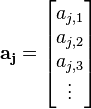
\includegraphics{images/Lecture_5/pic6.png}
      \end{minipage}
       
      \item Calculate the PDF for every key guess and save these for later. This might look like:
      \begin{minipage}{\linewidth}
      \centering
      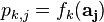
\includegraphics{images/Lecture_5/pic7.png}
      \end{minipage}
      \item Repeat these two steps for all of the attack traces
    \end{itemize}
    This process gives us an array of $p_{k, j}$, which says: ``Looking at trace j, how likely is it that key k is the correct one?"\\
    \textbf{Combining the Results}\\
    The very last step is to combine our $p_{k, j}$ values to decide which key is the best fit. The easiest way to do this is to combine them as:
    
    \begin{figure}[htp]
        \centering
        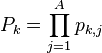
\includegraphics{images/Lecture_5/pic8.png}
       \end{figure}
    
    \subsection{practical template attacks}
    In this section we will show a differant ways to select the most important point of a power trace, that will lead us to improved computation time and make template attack more practical.\\
    \\
    \textbf{sum of difference}
       \begin{itemize}
          \item For every operation k and every sample i, find the average power $M_{k, i}$. For instance, if there are $T_k$ traces where we performed operation k, then this average is\\
              \begin{minipage}{\linewidth}
              \centering
              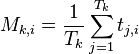
\includegraphics{images/Lecture_5/pic9.png}
              \end{minipage}
           
          \item After finding all of the means, calculate all of their absolute pairwise differences. Add these up. This will give one ``trace" which has peaks where the samples are usually different. The calculation looks like\\
          \\
              \begin{minipage}{\linewidth}
              \centering
              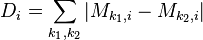
\includegraphics{images/Lecture_5/pic10.png}
              \end{minipage}
       \end{itemize}
        An example of this sum of differences is:\\
              \begin{minipage}{\linewidth}
              \centering
              \includegraphics{images/Lecture_5/pic11.png}
              \end{minipage}
        \\

\textbf{Preprocessing}\\
    In practical side-channel analysis, the raw input data is often preprocessed.
    Sometimes this is just due to simplicity or efficiency reasons, e. g. summarizing sampled points. There are however cases where the preprocessing step heavily affects the results. Even if no thinkable transformation can add additional information to a signal, information extraction procedures do improve. The template attack under consideration is such a case and a lucrative preprocessing transformation is described subsequently.
    It turns out that the transformation of the input traces from the time domain
    into the frequency domain is such a lucrative transformation. In our practical work, an FFT algorithm was used to accomplish this transformation (a fast algorithm to calculate the discrete Fourier transform, for background information refer to [BP85]). In order to show the impact of this preprocessing step a number of experiments were carried out. First some characteristic differences between time domain analysis and frequency domain analysis are illustrated. Afterwards, to highlight the influence of the number of selected points on the classification performance in the frequency domain, a number of experiments were carried out. After preprocessing, the resulting traces can be used to perform a template attack in exact the same way as without preprocessing. There is however a difference in the number of points to consider. Figure 6 shows the classifications results as a function of the number of selected points after preprocessing. The considered numbers of points are ranging between 1 and 40. Additionally three different minimum distances where chosen. Results show that much less points are sufficient in comparison to a template attack without the preprocessing step.
    At the price of performing an FFT on every input trace (those used to build
    up the templates as well as those to classify) we get a major advantage\\


\textbf{Amplified Template Attack}

    Even if the aim of a template attack is to recover the secret key using a single trace, in many real world settings implementations allow for several iterations of the same operation with the same secret key. The application of template attacks is not restricted to stream ciphers like RC4 and can be applied to block ciphers as well. Since every symmetric cipher contains some sort of key scheduling mechanism which processes the secret key, this generalization is possible. Smartcards often use block ciphers for encryption or authentication, hence let us consider the following example: A malicious petrol station tenant, named Eve, is using a modified smartcard based payment terminal. Everytime a customer uses this terminal, Eve captures one trace of side-channel information. This single trace could already be used by Eve to carry out a template attack.
    However, some customers are coming again and Eve gets hold of another
    trace. The template attack can easily be extended to take advantage of such
    situations, e.g. by adding up noise-probabilities p(Ni) of every captured trace and applying the maximum-likelihood approach on these sums. As a consequence, the power of the attacker is amplified. Using this approach, if n is the number of iterations, the error probability of template classification is reduced by the factor √n. 

\chapter{Introduction to micro-architectural attacks}
\label{chap:c7_cacheattacks}

Clementine Maurice, CNRS, IRISA\\
April 30, 2019 — Ben Gurion University, Israel

\section{Background \& Primitives} %arbel
\label{sec:BackgroundnPrimitives}

Micro-architectural side-channel attacks refers to a side-channel attack that exploit information leakage from the hardware infrastructure itself. The attacks can be found in a large scope on devices - servers, workstations, laptops, smart-phones, etc.

Normally, we assume a safe software infrastructure. Meaning that no software bugs, such as buffer overflow, is present. Nevertheless, such assumption does not imply safe execution, due to the fact that the information leaks because of the implementation, which is often driven by complex optimizations and design. Such leakages are not considered as 'mistakes' or 'bugs', but rather a trade-off decision between optimizing some aspects of the execution and potential information leakage.    

Potential outcomes of such attacks as described can be crypto primitives, which is common with other side-channel attacks, but also other sensitive information such as keystrokes and mouse movements.  

In terms of sources of leakage, we saw in previous chapters sources such as power consumption or electromagnetic leaks. However such sources are harder to come across by an attacker because they require physical proximity and access to the device, which is more typically to embedded devices. In our case we are only require that the attacker have somewhat remote access to the device, meaning that the attacker can run code on the hardware infrastructure of the machine. Such scenarios can be found in cloud providers renting computational resources to a costumer, Java-Script code running in a browser and others.

\subsection{Example: Cache attack on RSA Square-and-Multiply Exponentiation}
\label{subsec:CacheattackonRSA}

\begin{algorithm}
    \SetKwInOut{Input}{Input}
    \SetKwInOut{Output}{Output}
    \Input{base $b$, exponent $e$, modulus $n$}
    \Output{$b^e$ mod $n$}
    $X \leftarrow 1$
    \For{$i \leftarrow bitlen(e)$ \textbf{downto} $0$}
    {
    $X \leftarrow multiply(X,X)$
    \If{$e_i = 1$}
    {
    $X \leftarrow multiply(X,b)$
    }
    }
    \textbf{return} X
    \caption{Square-and-multiply exponentiation}
    \label{algo:SaM}
\end{algorithm}

Consider the binary exponentiation algorithm presented in Algorithm \ref{algo:SaM}. Notice that the execution flow of the algorithm relies heavily on the value of the bit $e_i$ of the private key. Now consider a scenario in which an attacker has information on the changes regarding the buffer holding the multiplier $b$. Such information can be considered as a query to the buffer and receiving as a result the latency of the query. If the buffer is in use, the query will be longer then if the buffer is unused.

\begin{figure}
    \centering
    \includegraphics[width=\textwidth]{images/PPSM.PNG}
    \caption{Querying the buffer holding the multiplier $b$. The y axis is a latency scale, and the x axis represent the query index. The dotted plot is a scatter plot while the solid line is the normalized moving average.}
    \label{fig:PPSQ}
\end{figure}

In \Cref{fig:PPSQ} the resulting graph of the querying can be seen, in which the actual bits of the exponent can be clearly detected.

\subsection{Attack Model}
\label{subsec:attackmodel}
We assume that the attacker has no physical access to the device. Moreover, the attacker can only execute unprivileged code on the same machine as victim. Such scenarios in which this happens can be found, for example, when the victim install some malicious program on his machine/smartphone. Another examples can be found in could computing where an attacker has a victual machine on the same physical machine as the victim, or in a web environment in which the attacker runs unprivileged JavaScript code.

In the scope of this chapter we will focus on shared hardware in the form of data/instruction cache. While other shared hardware components can also include the DRAM and the memory bus (memory shared hardware) or the branch prediction unit and the arithmetic logic unit (CPU shared hardware), they are not in the scope of this chapter.

\subsection{Today's CPU Complexity}
\label{subsec:todaycpucomplex}
From 2012 onwards Intel has released a new family of microprocessors every year. Each comes with its own new microarchitectural schemes with new Characteristics. To gain performance upgrade in each new installment, that has on average 5\% increase in performance depending on the feature, very small optimizations, such as caches and branch prediction units are added. Such optimizations are the main reason for a side-channel information leakage to exist. Unfortunately, said optimization often come with no documentation since this is Intel intellectual property. Such lack in documentation makes it harder for an attacker to perform said side-channel attacks.

To emphasize today's CPU complexity, it is said that ``Intel x86 documentation has more pages than the 6502 has transistors" \cite{IntMan}, with 6502 being a reference to a 8-bit microprocessor, used in Apple II, Commodore 64, Atari 800 and more. It had, in the year 1975, roughly 3510 transistors, while the Intel Software Developer's Manuals is 4844 pages (may. 2018). In a more advance microprocessor, such as the 22-core Intel Xeon Broadwell-E5, more than 7 billion transistors can be found. 

\subsection{Background on Caches}
\label{subsec:backgroundoncaches}
In designing a cache side-channel attack, a proper understanding of how caches work, in great detail, is required. First, we need to acknowledge that the requirements for an 'ideal memory' oppose each other. Such requirements are zero latency, infinite capacity, zero cost and infinite bandwidth. The trade-offs are interconnect: \textbf{Bigger is Slower} - Bigger memory often comes with higher latency, due to the fact the it would take longer to determine the location to retrieve.  \textbf{Faster is Expensive} - A reduction in latency often means that a more expensive technology a needed. For example, SRAM is faster than DRAM, which in turn is faster than Disk memory. However, their cost ratio is the other way around. \textbf{Bandwidth is Expensive} - A wider bandwidth needs to come with additional banks, ports, higher frequency or faster technology. 

In our need to understand the use of caches, we need to examine the different memory technologies and why they are used the way they do. \textbf{DRAM} - Dynamic Random Access Memory is the technology that is often used as the main memory (or RAM), while \textbf{SRAM} - Static Random Access Memory is the technology used in caches. The DRAM latency is higher than the SRAM latency, but is cheaper to make. The main difference in cost arises from the fact that DRAM consist only of one transistor and one capacitor per cell, while the SRAM consist of six transistors per cell. Said difference also mean that DRAM is more dense. Finally, the DRAM cell layout and technology requires to periodically refresh each cell.

Since having Both a large and fast, single level of memory is unlikely, CPU's today are made with multiple levels of storage. The main idea is that progressively bigger and slower storage units are located in higher levels of memory, which are farther from the processor. The motivation for such design is to ensure that most of the data the processor needs is kept in the closer and faster levels.

\begin{figure}
    \centering
    \includegraphics[width=\textwidth]{images/MemHier.PNG}
    \caption{Memory Hierarchy of a common CPU.}
    \label{fig:MemHier}
\end{figure}

The memory hierarchy can be seen in \Cref{fig:MemHier}, where data can reside in, at a given point in time, in the following storage units - in CPU registers, the different levels of the CPU cache, main memory or disk memory. 

\subsection{Caching Basics}
\label{subsec:cachingbasics}
The two main idea of caching is to exploit temporal and spatial locality. \textbf{Temporal Locality} is the notion that a program tends to reference the same memory location many times within a small window of time (for example, loops). The anticipation of such thinking is that recently accessed data will be accessed again soon. Therefor, a good strategy will be to store recently accessed data in automatically managed fast memory. \textbf{Spatial Locality} is the notion that a program tends to reference a cluster of memory locations at a time (for example, sequential instruction access or array traversal). The anticipation will be that surrounding of some accessed data will be accessed soon. A good strategy will consider storing addresses adjacent to the recently accessed one in an automatically managed fast memory. In detail, we want to logically divide memory into equal size blocks (lines) and fetch to cache the accessed block in its entirety.   

Moreover, there are two approaches to the management scheme, manual and automatic. \textbf{Manual Management} means that the programmer manages data movement across levels, which is not scalable for substantial programs. However, it is sometimes used in some embedded systems. \textbf{Automatic management} refer to a scheme in which the hardware itself manages data movement across the different levels in a way that is transparent to the programmer. Meaning that the average programmer does not need to know anything related to the memory hierarchy levels to write a program. On the down side, which begs the question on how to write a fast program if the management is automatic, in addition to what kind of side-channels could arise from such scenario.

The basic unit of storage in the cache is called a block or a line. The main memory is logically divided into cache blocks that map to locations in the cache. And when data is referenced, two outcomes can come of such action - a cache hit or a cache miss. A \textbf{Cache Hit} occurs when a line is referenced and is in the cache. The cached data will be retrieved instead of accessing main memory.  A \textbf{Cache Miss} occurs when a line is referenced and is not in the cache. The data will be fetched from main memory, passing though the cache, possibly eviction other data to ensure enough storage.

When designing a cache, we are faced with a number of design decisions to handle. \textbf{Placement}  - Essentially the place in which we will place or find a block in the cache. \textbf{Replacement} - We need often to remove data from the cache to make room for newer data. Which begs the question of what data to evict. \textbf{Granularity of Management} - The basic units of storage in different levels. Do we store the same amount of blocks across different levels or do we uniformly store the same size of blocks. \textbf{Write Policy} - When a write is being made, we need to decide whether to preform the write operation in all levels or passing the write data to a lower level only upon eviction from that level. \textbf{Instruction/Data} - When a program is executing, the instructions that are in need to be executed are required to be fetched from memory as well. The designer needs to decide whether to treat instruction and data memory as two separate  types or as one of the same.


\subsection{Set-Associative Caches}
\label{subsec:setassoccaches}

We will be focusing on a cache design that is often used in today's CPUs, which is set-associative caches. Which means that the cache will be logically divided into \textbf{Cache Sets}, which will be divided into \textbf{Cache Ways}. Each way will store a cache line worth of data. The division of the memory into different cache sets will be a direct mapping from the memory address. Namely, each address will be associated with a cache set according to a group of bits in the address which will represent the cache set index. The specific way in which the line will is to be fetch will be determine according to the cache replacement policy, since the cache set is expected to be full.  An
abstraction can be seen in \Cref{fig:SetWay}


\begin{figure}
    \centering
    \includegraphics[width=\textwidth]{images/SetWay.PNG}
    \caption{Set-Associative Cache - The set index of a line derives from the set index bits of the address. The cache way is determine according to the cache replacement policy.}
    \label{fig:SetWay}
\end{figure}

Consider the following example: The cache has 8B cache lines, 16 cache sets each consisting of 2 ways. We can compute the set index of the address $(1011111110)_b$ by only looking at bits $b_3, b_4, b_5, b_6$, since we have 16 cache sets (4 bits) and 8 different cache line offset (bits $b_0, b_1, b_2$). Hence the cache set will be $(1111)_b$. We can also compute the size of the whole cache by multiplying the cache dimensions $8 \times 16 \times 2 = 256 $B.

\subsection{Virtual Addresses or Physical Addresses}
\label{subsec:addrorphysicaladdr}
Since we need the bits of address to determine its cache set, we are face with a problem due to the fact that programs running are only aware to the virtual addresses while the hardware side is aware to the physical addresses. The translation between virtual addresses and physical addresses is the responsibility of the MMU (Memory Management Unit).

There are four major ways of implementing such cache mapping according to the addresses. \textbf{VIVT} - Virtually-Indexed, virtually-Tagged. Meaning that there is no need to translate the addresses in order to know the mapping of the addresses into the cache, which is faster. On the other hand, such implementation causes aliasing issues as same virtual address maps to several different physical addresses. This aliasing is due to the tag not being unique, and will force a flush action to the entire cache on context swiching. \textbf{VIPT} - Virtually-Indexed, Physically-Tagged. Meaning that there will be a need for TLB translation for the tag, but can be looked up in parallel. Such mapping can be quiet fast. Moreover, if the set index bits are derived from the page offset, there is no aliasing, but the cache size is limited to the page size multiply by the number of cache sets. VIPT is used in Intel's L1 caches, with the default page size being 4K and each cache line is 64B, resulting in no larger than $2^6 = 64$ sets. \textbf{PIPT} - Physically-Indexed, Physically-Tagged. Meaning that the translation between virtual and physical addresses will have to be preformed, taking up time. On the other hand, no aliasing issues occurs and no required  limitation on the number of sets is present. Typically used in the larger Intel caches - L2 and L3. \textbf{PIVT} - Physically-Indexed, Virtually-Tagged. Meaning that all the limitations of previous ways apply, and is rarely used in practice. 

\subsection{Replacement Policy} 
\label{subsec:replacementpolicy}
We need to decide on a policy according to which a cache line will be evicted in order to make room for incoming data. Many replacement policies exist, namely FIFO (first in, first out), LRU (least recently used), LFU (least frequently used), random, a hybrid and more.

Intel commonly applies a LRU policy or a pseudo-LRU policy (since pure LRU is complex to implement). Which determines that the oldest cache line to be referenced will be evicted, As if each cache line is attached with a time-stamp that is updated on access. An example can be thought of by having $n$ way cache set and $n+1$ different lines of memory that are mapped into said cache set and are accessed in order. The first $1,\dots,n$ lines will fill the cache ways, while the $n+1$ access will evict the first memory line from the set, since all the set ways are full.  

A potential issue arises with LRU policy when a program need to access cyclically $n+1$ memory lines (``program working set") that are mapped to the same $n$ way cache set. This is referenced as a 'set thrasing' and will result in $0\%$ hit rate. If we compare LRU policy to a random policy, depending on the workload, some studies have shown that LRU and random replacement policies have the same hit rate on average.

When implementing a cache side-channel attack, we will normally will want to evict some special memory location from the cache. Considering a non-LRU replacement policy will mean that evicting a memory line from the cache will not necessarily be practical, since there is no guaranty that if the attacker access memory locations in a specific pattern we will evict the whole set from the cache. 
\subsection{Caches on Intel CPUs}
\label{subsec:cachesonintelcpus}
\begin{figure}
    \centering
    \includegraphics[width=\textwidth]{images/IntelCPU.PNG}
    \caption{Basic Intel CPU - each core has its own L1 and L2 caches, while all connected to a larger sliced L3 cache which can be accessed from all cores. }
    \label{fig:IntelCPU}
\end{figure}

In \Cref{fig:IntelCPU} we can see an abstraction of an Intel CPU architecture, on which every core has its own dedicated L1 instruction and data cache, in addition to a slightly bigger L2. All cores are connected via an interconnected bus to the last level cache (LLC/L3). The LLC often is sliced intro the number of cores, having a dedicated slice to each core, while having all cores being able to access all slices. The common practice is that the different levels of caches are inclusive, meaning that a lower level cache is a super-set of the higher ones.  

In order to preform a cache side-channel attack, an attacker can optimize its cache usage, among other things, using the following command: \texttt{prefetch} - A suggestion to the CPU that some memory line will be accessed soon, can trigger fetching that line into the cache by the CPU. \texttt{clflush} - Cache line flush, instructs the CPU to flush a memory line from all levels of the cache. The two instructions are based on virtual addressed.

The different latencies of the different cache levels, as well as the timing difference between a cache miss and a cache hit, as can be seen in \Cref{fig:cache_hits_misses_hist}, are the main primitives of most cache side-channel attacks that will be discussed by the end of this chapter.  

\section{Cache Attacks Techniques} %ben
\label{sec:cacheattackstech}

Microarchitectural attacks exploit hardware properties that allow inferring information on other processes running on the same system.
In particular, cache attacks exploit the measurable timing difference between the CPU cache and the main memory. They have been the most studied microarchitectural attacks for the past 20 years, and were found to be powerful to derive cryptographic secrets \cite{Percival2009}. In such attacks, the attacker monitors which memory lines are accessed, not the content of a certain memory line.

\noindent Cache attacks are being used in one of the two following common scenarios:
\begin{itemize}
\item \textbf{Covert channel}: two processes communicating with each other when they are not allowed to do so, e.g., across VMs.
\item \textbf{Side channel attack}: one malicious process spies on benign processes, e.g., steals crypto keys, spies on keystrokes etc. 
\end{itemize}
We will focus on side-channel attacks.

\subsection{Cache Side-Channel Timing Attacks}
\label{subsec:cachesidechanneltiming}
Every timing attack works by the following steps:
\begin{enumerate}
    \item Learn timing of different \textit{corner cases}.
    \item Recognizing these corner cases by timing only.
\end{enumerate}
Here, our corner cases are \textit{hits} and \textit{misses}.

\subsubsection{Building the Histogram}
\label{subsubsec:buildingthehistogram}
The first step towards the attack is to build the histogram of the corner cases, cache hits and cache misses. We measure the time for each case many times in order to get rid of noise. Thus, we have a histogram and we can find a threshold to distinguish the two cases.

\noindent Building the histogram for cache hits is done by the following loop:
\begin{enumerate}
    \item Measure time.
    \item Access variable (always cache hit).
    \item Measure time again.
    \item Update histogram with delta.
\end{enumerate}

\noindent Building the histogram for cache misses is done by the following loop:
\begin{enumerate}
    \item Flush variable (\texttt{clflush} instruction).
    \item Measure time.
    \item Access variable (always cache miss).
    \item Measure time again.
    \item Update histogram with delta.
\end{enumerate}

\noindent Having the two histograms, as in \Cref{fig:cache_hits_misses_hist}, we determine the threshold to be as high as possible such that there will be no cache miss below. 
\begin{figure}[!ht]
    \centering
    \includegraphics[width=\textwidth]{images/cache_hits_misses_hist.JPG}
    \caption{Timing differences histogram of cache hits and cache misses.}
    \label{fig:cache_hits_misses_hist}
\end{figure}

\subsubsection{How to Measure Time Accurately}
\label{subsubsec:howtomeasuretimeaccuractely}
Consider the fact that the time intervals of our cases is (relatively) very short timings, we ask how to measure time accurately. For such short timings, it is common to use the Time Stamp Counter (TSC) via the unprivileged \texttt{rdtsc} instruction as following:
$$[...] \rightarrow \texttt{rstsc} \rightarrow \mbox{function()} \rightarrow \texttt{rstsc} \rightarrow [...]$$
\noindent By using this instruction, due to out-of-execution, the actual execution order could be different, resulting with wrong measurements. The solution is to use the pseudo-serializing instruction \texttt{rdtscp} or to insert a serializing instruction like \texttt{cpuid} or use to fence instructions like \texttt{mfence} \cite{benchmark2010}.

We will now introduce two cache attack (main) techniques: Flush+Reload \cite{Gullasch:2011:CGB:2006077.2006784, Osvik:2006:CAC:2117739.2117741, Yarom2014} and Prime+Probe \cite{Percival2009,Osvik:2006:CAC:2117739.2117741,Liu:2015:LCS:2867539.2867673}. Both of them are exploitable on x86 and ARM and can be used for both covert channels and side-channel attacks.
\subsection{Flush+Reload}
\label{subsec:flushreload}
The attack is made of four basic steps and it goes as following:
\begin{enumerate}
    \item \textbf{Map. } The attacker maps a shared library (Illustration in \Cref{fig:fr_sharedlib}), by doing that he will have a shared cache line with the victim.
    \item \textbf{Flush.} The attacker \textit{flushes} the shared cache line, it can be done via unprivileged instruction like \texttt{clflush}.
    \item \textbf{Victim.} The attacker lets the victim load (or not load) the shared line, depending on the victim's behaviour.
    \item \textbf{Reload.} The attacker reloads the shared cache line. If the cache line has a \textit{hit} the attacker infers that the victim loaded the data on the previous step, if the cache line has a \textit{miss} the attacker infers that the victim did not load the data on the previous step.
\end{enumerate}

\begin{figure}[!ht]
    \centering
    \includegraphics[width=\textwidth]{images/fr_sharedlib.JPG}
    \caption{Attacker maps shared library (shared memory, in cache), shared cache line marked in red}
    \label{fig:fr_sharedlib}
\end{figure}

\begin{figure}[!ht]
    \centering
    \includegraphics[width=\textwidth]{images/fr_flow.png}
    \caption{Flush+Reload attack flow. Between the first flush and the first reload the victim did not access the shared cache line, so the first reload resulted with a cache hit. Then, after the second flush the victim accessed the shared cache line and hence, the second reload resulted with a miss.}
    \label{fig:fr_flow}
\end{figure}

\noindent The first step (Mapping a shared library) can be done once, while steps 2-4 are repeatable as much as the attacker wants. The main advantage of this attack technique is the fine granularity, which is 1 memory line (usually 64B). On the other hand, this technique is somewhat restrictive, it needs \texttt{clflush} instruction, which is not always available e.g., on ARM-v7 and it needs a shared memory. Illustration of the attack flow in \Cref{fig:fr_flow}.

\subsubsection{Shared Memory}
\label{subsubsec:sharedmemory}
Common method to achieve a shared memory is by a feature called \textit{page-deduplication}. When two different independent processes are loading the same system library, some of their memory pages will be identical, when the operating system (in a cloud scenario - the hypervisor) identify separate identical physical memory pages, if page-deduplication is enabled, it will merge the physical pages in order to save physical memory, and two different virtual memory pages, one of each process, will be mapped into the same physical memory page. As of today, no cloud service company that takes itself seriously is using memory deduplication, e.g., Amazon EC2.

\subsection{Prime+Probe}
\label{subsec:primeprobe}
First, for the Prime+Probe attack to work, the Last-Level-Cache (LLC) should be inclusive, i.e., the LLC is a superset of the L1 cache and the L2 cache. Thus, data evicted from the LLC is also evicted from L1 and L2.
In inclusive caches, a core can evict lines in the private L1 of another core.
The attack is made of the three following steps:
\begin{enumerate}
    \item \textbf{Prime.} The attacker primes the cache by reading memory lines from its own exclusive memory (no shared memory).
    \item \textbf{Victim.} The attacker lets the victim evict (or not evict) lines while running, depending on the victim's behaviour.
    \item \textbf{Probe.} The attacker probes data in a similar way of the prime step but with measurement of how much time it takes to load the lines (Hit / Miss), for each cache set, the attacker determine if the cache set has been accessed.
\end{enumerate}

\begin{figure}[!ht]
    \centering
    \includegraphics[width=\textwidth]{images/pp_flow.JPG}
    \caption{Prime+Probe flow.}
    \label{fig:pp_flow}
\end{figure}

\noindent In compare to Flush+Reload, this attack technique is less restrictive: it does not require \texttt{clflush}, does not assume shared memory and possible from JavaScript. On the other hand, the granularity is coarser: 1 set.  Illustration of the attack flow in \Cref{fig:pp_flow}.

In practice, we need to evict caches lines without \texttt{clflush} or shared memory, so the following questions arise:
\begin{itemize}
    \item Which addresses do we access to have congruent cache lines?
    \item How do we do that without any privilege?
    \item In which order do we need to access them?
\end{itemize}
For doing that, we need an \textit{eviction set}: addresses in the same set, in the same slice and an \textit{eviction strategy}.

\subsubsection{Eviction Set}
\label{subsubsec:evictionset}
\footnote{From now on, most of the details are correct for a common Intel CPU architecture.}
We want to target the L3 for cross-core attacks and we need addresses that have the same set index. Consider the following cache settings, L3 for a 2-core CPU: 4096 sets, 64B-lines, 12 or 16 ways. Since each memory address indicates one memory byte, the 6 least significant bits of the physical address indicate the line offset. For the sake of simplicity, we assume that the cache is not sliced, since there are $4096=2^{12}$ cache sets, the next 12 bits indicate the cache set. The L3 is physically indexed, so we need to choose addresses with fixed physical address bits. Unfortunately, address translation from virtual to physical is privileged. One of the properties of a virtual address is that a page offset stays the same from virtual to physical address, thus, some of the least significant bits of the virtual address can be used as a sneak peak to the physical address. A typical page size is 4KB, which means just 12 bits of page offset, i.e, 6 bits of line offset and 6 least significant bits of the cache set out of 12. To overcome this limitation, we can use a special type of enlarged pages called \textit{Huge Pages} which are 2MB size each, that is - 21 bits of page offset. This way the set index bits are included in the 21 LSB of the address.

We now have another issue, in practice, the L3 is divided in slices, as many slices as cores. We usually have 2048 sets per slice, that is, actually 11 bits for the set index. We cannot infer the slice number directly from the address, neither from the virtual or the physical. The slice number of each memory line is determined by a hash function which takes all the address bits as input, including physical page number bits (outside the known bits from page offset). Illustration of which bits of the address indicates what for both typical pages and huge pages is shown in \Cref{fig:slicedcache}.

\begin{figure}[!ht]
    \centering
    \includegraphics[width=\textwidth]{images/slicedcache.JPG}
    \caption{Sliced cache.}
    \label{fig:slicedcache}
\end{figure}

In addition, the mentioned hash function is undocumented, it designed for performance. But, it does not mean that it is impossible to target the same set in the same slice. Previous work \cite{EURECOM+4671} showed that the hash function can be reverse engineered, for example in \Cref{fig:hashfunc}.

\begin{figure}[!ht]
    \centering
    \includegraphics[width=\textwidth]{images/hashfunc.JPG}
    \caption{Three reversed engineered hash functions, depending on the number of cores. Function valid for Sandy Bridge, Ivy Bridge, Haswell, Broadwell}
    \label{fig:hashfunc}
\end{figure}

If the function is unknown, the process will be somewhat slower. But an eviction set can still be achieved via the following algorithm:
\begin{enumerate}
    \item Construct $S$, set of addresses with the same set index.
    \item Access reference address $x \in S$ (to load it in cache).
    \item Iteratively access all elements of $S$.
    \item Measure $t_1$, the time it takes to access $x$. it should be evicted.
    \item Select a random address $s$ from $S$ and remove it.
    \item Iteratively access all elements of $S$\textbackslash$s$.
    \item Measure $t_2$, the time it takes to access $x$ - is it evicted?
    \begin{itemize}
        \item If not, $s$ is part of the same set as $x$, place it back into $S$.
        \item If it was evicted, $s$ is not part of the same set as $x$, discard $s$.
    \end{itemize}
\end{enumerate}
\noindent Note that for a CPU with c cores: $16/c$ addresses in the same set and slice per 2MB page, we can apply the same algorithm with groups of addresses instead of single addresses and speed up the eviction set building process by up to three orders of magnitude.

\subsubsection{Eviction Strategy}
\label{subsubsec:EvictionStrategy}
In the Prime or the Probe step, the attacker evicts a cache set by filling it with $n$ addresses for a $n$-way cache. If the replacement policy is LRU, it access addresses from eviction set 1 by 1. If the replacement policy is not LRU, the eviction rate is lesser than $100\%$, e.g. $75\%$ on Haswell. For non-LRU caches, we can use some heuristics, as in \Cref{fig:haswellstrategy}, that will result with a higher eviction rate.

\begin{figure}[!ht]
    \centering
    \includegraphics[width=\textwidth]{images/haswellstrategy.JPG}
    \caption{$a_1\dots a_9$ are in the same cache set. Fast and effective on Haswell: eviction rate $> 99.97\%$}
    \label{fig:haswellstrategy}
\end{figure}

\subsubsection{Conclusion}
\label{subsubsec:Conclusion}
To sum it up, in practice, for Prime+Probe on recent processors we need:
\begin{itemize}
    \item An eviction set, i.e., addresses in the same slice and with the same set index. Depends on the addressing.
    \item An eviction strategy, i.e., the order with which we access the eviction set. Depends on the replacement policy
\end{itemize}

\subsection{Hardware vs. implementations}
\label{subsec:Hardwarevsimplementations}

To perform a cache side-channel attack on some software you need two things: First, shared and vulnerable hardware. Note that there will be no side channel if every memory access takes the same time or if you cannot share the hardware component. Second, a vulnerable implementation. Note that a vulnerable implementation doesn't mean that the algorithm is vulnerable. For example, we can take specific implementation of AES and RSA, this doesn't mean that AES and RSA are broken. Not all implementations are created equal.

To sum up, hardware will most likely stay vulnerable, so patch implementations when you can. And remember, constant time is not enough - because an attacker can modify the internal state of the micro-architecture.

\section{Step by Step Attack Demo} %yaniv
\label{sec:stepbystepattack}

The target of the attack in this demonstration, is to get the timestamp of the keystrokes pressed by a user in a gedit program. We only target the timestamps and not the keystrokes themselves, as we are not able to fully recover the pressed keys.

The demonstration is performed on a non-virtualized Linux environment. A requirement to perform the attack is having an Intel CPU, as we need the inclusive property of L3 cache. The code for performing the attack can be cloned from the git repository \cite{GitClementine}. It is based on the Flush+Reload cache attack that we mentioned in \cref{subsec:flushreload} presented in \cite{Yarom2014} and \cite{Gruss2015}.

The attack is performed in 3 steps: calibration, profiling and exploit. For each of these steps, a folder exists in the repository.

\subsection{Step 1: Calibration}
\label{subsec:step1calibration}

In this step we want to create the histogram which depicts the cache misses and hits as a function of the number of CPU cycles. Then we will be able to extract the threshold that will match the CPU on which we perform the attack.
In order to perform the calibration, we run the following commands:

\begin{lstlisting}[language=bash]
  $ cd calibration
  $ make
  $ ./calibration
\end{lstlisting}

The calibration works by generating multiple cache misses and cache hits, and measuring the number of CPU cycles it takes to access a variable. Each of these cases is being performed multiple times in order to get rid of the noise.

\noindent We build a histogram of cache hits and cache misses as described in previous \cref{subsubsec:buildingthehistogram}. The output of the calibration program is a histogram of the cache misses and hits as shown in \Cref{fig:cache_hits_misses_hist}.

We can then find the threshold so it satisfies the following requirements:
\begin{enumerate}
    \item As high as possible
    \item Most cache hits are below it
    \item No cache miss below (we may see one exception due to the way the calibration is coded)
\end{enumerate}

For example, in \Cref{fig:cache_hits_misses_hist}, we can see that there is a clear line in approximately $220$ CPU cycles.

\subsection{Step 2: Profiling}
\label{subsec:step2profiling}

After finding the threshold, we can now profile in order to find the cache lines that are actually useful to get information about the target program. Choosing gedit as the target program, we first need to find the shared library that it uses, so we can give it as an input to the profiler. We then need to find this shared library file location and size. In order to do that, we can use the following one-liner:
\begin{lstlisting}
$ cat /proc/`ps -A | grep gedit | grep -oE "^[0-9]+"`/maps | grep r-x | grep libgedit
\end{lstlisting}
This is equivalent to first finding the pid with
\begin{lstlisting}[language=bash]
  $ ps -A | grep gedit
\end{lstlisting}
and then using this pid in
\begin{lstlisting}[language=bash]
  $ cat /proc/<pid>/maps | grep libgedit
\end{lstlisting}
then copying the line with r-xp permissions (x stands for executable).

Doing that gives the following line (memory range, access rights, offset, –, –, file name):

\begin{lstlisting}[language=bash]
7f2d83197000-7f2d8326d000 r-xp 00000000 08:02 1080575             /usr/lib/gedit/libgedit.so
\end{lstlisting}

Before we can feed the above line to the profiler, we need to update the threshold to the value we found in the calibration step. We can do this by editing the profiler source file (under the profiling directory) and updating the line with the constant 
\begin{lstlisting}[language=bash]
#define MIN_CACHE_MISS_CYCLES
\end{lstlisting}
to the threshold we have.

After updating the threshold, we can run \texttt{make} to compile the profiler. We then use \texttt{sleep 3} so we can have time to trigger the event before the profiler starts, and run the profiler with the line we found above: 
\begin{lstlisting}[language=bash]
sleep 3; ./profiling 200 7f2d83197000-7f2d8326d000 r-xp 00000000 08:02 1080575                    /usr/lib/gedit/libgedit.so
\end{lstlisting}

The profiler does its job by loading the shared library to its address space, and then doing flushes and reloads for each address in the address range given by the offset argument (0 in the above case), and the library size (1080575 bytes) for some given time (200 $\mu$sec for every address in the above command). The output is the number of hits that happened in every address.

The idea is that if a 0 is shown for a given address while triggering the event, then it means that the line in this address was never accessed for this event. Eventually, we will get lines with a number of cache hits, and we want the ones that have at least a non zero value when profiling.

\begin{figure}[!ht]
    \centering
    \includegraphics[width=\textwidth]{images/profiling-cache-hits.png}
    \caption{Addresses with cache hits.}
    \label{fig:profiling-cache-hits}
\end{figure}

Running the profiler with offset 0 while jamming a key, doesn't seem to generate cache hits, and we may only see 0. The reason for that, is that the code that handles keystrokes in the library is probably just not in the beginning of the library. Instead (and this is a cheat), we change the starting offset to 20000, and this is approximately where the code that handles keystrokes in the library is found. In real life we will have to wait until we get to something by running the template attack on the whole library. Running the profiler with this new offset, we can see in \Cref{fig:profiling-cache-hits} some addresses that have a non-zero value quite fast. The addresses with the high numbers are the ones we should further investigate in the exploit phase.

\subsection{Step 3: Exploitation}
\label{subsec:step3exploitation}

Equipped with the addresses from the previous step, we can now go to the exploitation dir, change the threshold constant (MIN\_CACHE\_MISS\_CYCLES) as we did for the profiler, and run \texttt{make}. Then we can run the program by 
\begin{lstlisting}[language=bash]
./spy <library-file> <offset>
\end{lstlisting}
giving one of the addresses we found as the offset argument. Starting from the address with the most hits, we can see that even if we are not pressing any key, we are still getting events. The reason for that is that this address is related to the blinking cursor. This is, of course, not really interesting information, and we can understand that it's not always the address that has the most hits that is the most valuable. Trying the next interesting address indeed gives us information about the pressed keys, which is what we wanted to achieve. However, moving the mouse also gives us a lot of hits, which is not perfect. What we will need to do is to inspect the addresses one by one until we find an address that will only work for keystrokes.

We can even further improve the attack by finding the complete matrix of the keystrokes for each of the keys as shown in \Cref{fig:cache-keymap-matrix}. We can see that for different keys, there is a different “signature” of the accessed addresses. Although we may not be able to identify each keystroke precisely, we can try to group the keystrokes to different addresses and eliminate some guesses if we are able to spy on more than one address at a time.

\begin{figure}[!ht]
    \centering
    \includegraphics[width=0.8\textwidth]{images/cache-keymap-matrix.png}
    \caption{Complete matrix for each keystroke.}
    \label{fig:cache-keymap-matrix}
\end{figure}

Finally, as it may be annoying to perform the above process manually, we can automate the event triggering and other stuff as shown in \cite{GitGruss}.

\chapter{Fault Attacks}\label{cha:c9_ninthchapter}

\begin{centering}
	\section*{Topics}\label{sec:topics}
		\begin{enumerate}
			\begin{centering}
				\item Introduction to Fault Attacks
				\item Fault Attack on RSA-CRT
				\item DRAM and Rowhammer
				\item Flip-Feng-Shui: Rowhammer attack on RSA \\
			\end{centering}
		\end{enumerate}
\end{centering}
\newpage

\section*{Introduction to Fault Attacks}\label{sec:introduction_to_fault_attacks}
Up until now in the course we learned about \emph{passive} attacks -- i.e.\ attacks which measure \emph{leakage} such as timing information and power traces. The advantage of these attacks is that they allow an attacker to acquire information in the process of an ongoing computation e.g.\ an AES key \emph{before} it was fully mixed with the input -- this fact can help the attacker extract secrets.

In fault attacks we will become \emph{active} in the sense that we will give the device-under-test (DUT) additional inputs such as heat or radiation.

One problem with Fault attacks: they use the strongest attack model, meaning -- we assume most power on the attacker's part.

\section{Active Attacks}\label{sec:active_attacks}
\paragraph{Definition:}
\begin{quote}
	\textit{``A faul attack is an active attack that allows extraction of secret information from cryptographic devices by breaking those devices.''}
\end{quote}

In fault attacks we are being \emph{active} -- we give additional inputs beside the main input such as:
\begin{enumerate}
	\item Fuzzing (garbage or bad input)
	\item Radiation
	\item Heat
	\item Vibration
	\item Power spikes etc.
\end{enumerate}

This way, we receive other (usually erroneous) outputs which might give us additional information about the computation and/or the secret. This process is described in \Cref{fig:fault_attacks_schematic}.

\begin{figure}[!ht]
	\centering
	\includegraphics[width=0.7\linewidth]{images/chapter_9/fault_attacks_schematic.png}
	\caption{A schematic diagram of fault attacks and leakage types.}\label{fig:fault_attacks_schematic}
\end{figure}

Like with passive attacks, some of those outputs can be acquired at different stages of the computation process.

Many fault attacks are inspired by studies in the field of \emph{reliability}: a study in reliability will research a device's physical boundaries e.g.\ the maximum or minimum temperature under which it performs reliably. Other examples of reliability studies are aimed at improving device performance under extreme conditions such as:
\begin{itemize}
	\item Space and X-Rays
	\item Dense CPU Layouts
	\item Data Center Recovery (ECC-RAM)
\end{itemize}

A security researcher implementing fault attacks will, on the other hand,  purposefully subject the DUT to extreme conditions in order to inject errors in the device's functionality to achieve their goal. In that sense, a reliability study of a given device can lay the ground-work for the fault attacks to come.

\begin{quote}
	\textit{``In the reliability community things happen by mistake. In the security community -- things happen on purpose.''}
\end{quote}

\subsection*{Breaking a device-under-test}\label{subsec:breaking_a_device_under_test}
How can \emph{breaking} a device help an attacker?

\begin{enumerate}
	\item BORE -- \textit{``Break Once, Run Everywhere''}: Some device families share a single secret among all instances.
	\item Repairable Devices: Temporary breakage is fine. Sometimes restarting the device is enough to ``repair'' the damage.
	\item Partial breakage: Sometimes it's convenient to break \emph{part} of a device, for example -- destroy the subsystem responsible for DRM verification.
\end{enumerate}

\section{Fault Attack Taxonomy}\label{sec:fault_attack_taxonomy}
The tree ways we can examine a Fault Attack in order to understand it are:
\begin{enumerate}
	\item Method - \emph{``How to inject?''}
	\item Properties - \emph{``What fault to create?''}
	\item Target - \emph{``Which part to break?''}
\end{enumerate}

\subsection{Fault Methods}\label{subsec:fault_methods}

\subsubsection{Power Supply Attacks}\label{subsubsec:power_supply_attacks}
What happens if the device is underpowered?
As we have previously seen, power in electronic devices is used to drive the CMOS transistors. If the device is slightly underpowered it might fail to switch some of the transistors and thus produce false calculations, and with even less power it might  struggle with getting into operational state (boot loop) or even transition to an entirely faulty state.
Another attack method involving the power supply is injecting power spikes (to a similar effect).

Some parts of a device are typically more sensitive to the power supply than others, and thus under- or over-powering the device will de-stabilize it and inject faults.

The obvious scenario for such an attack is when the DUT belongs to or is being controlled by the attacker -- for example if they're examining their own set-top box etc. In that case, the attacker can supply the device with as much/little power as they wish.

Another example of such attack scenarios is in the field of RFID readers -- the device powering an RFID chip is the reader, so a \emph{malicious} RFID reader can over/under-power the chip to achieve various faulty results.

\subsubsection{Clock/Timing Attacks}\label{subsubsec:clock_timing_attacks}
The clock is typically a bus shared by many of the system's components which synchronizes the propagation of calculations through the system -- i.e.\ at the beginning all inputs are ready, and when there is a rising edge on the clock bus they start propagating throughout the various computational components. When all computations are finished they all wait for the next rising edge on the clock bus in order to proceed to the next stage.
In a clock glitching attack the attacker would inject a rising edge on the clock bus at an arbitrary time. This way only \emph{some} of the computations will have finished by that time while others are still being processed, and thus the device will be in a faulty (unstable) state.

A notable example is the attack on Mifare Classic RFID chips we talked about in the beginning of the course~\cite{nohl2008} -- the RNG in the chip is only dependent on the time between powering up the RFID tag and challenging it. An RFID reader operated by the attacker can control both parameters, thus making the generated challenges deterministic.

\subsubsection{Temperature attacks}\label{subsubsec:temperature_attacks}
This attack method relies on the physical property of electrons (current). Electrons ``jump'', and the higher the temperature -- they will jump more frequently and to longer distances.
If a device gets \emph{too hot} -- enough electrons can ``jump'' e.g.\ over the insulation layer in a transistor to flip it from logical 1 to 0. This results in a fault.

Because of the ubiquity of devices failures due to temperature, nowadays temperature sensors are integrated into most devices, so when it overheats -- the device will shut down.

An attacker can bypass the temperature sensor by disconnecting it. Another method would be to quickly alternate the temperature of the device from extremely high to extremely low, so that \emph{on average} the temperature is reasonable, but it will still experience faults during the extreme phases of the cycles.

In an interesting research paper~\cite{appel} a type-confusion attack on the 
Java virtual-machine was demonstrated: at first, the entire memory was filled 
with small arrays (say of size one). The Java VM is type-safe, so it is 
normally impossible to access one of the memory regions using a pointer to a 
different region. To inject a type-confusion fault the researchers used a 50W 
light bulb to heat the memory chip of the device enough to flip some of the 
bits (for illustration see \Cref{fig:memory_lightbulb}). As a result, a small 
portion of the data-structures describing the arrays in memory now held wrong 
values (e.g.\ changed their value from \(size=1\) to \(size=20\)). At this point, 
some affected data-structure \emph{contains} a header of a different 
data-structure, to which the attackers now have read and write access. Changing 
the header of the second data structure to an arbitrary value gave the 
attackers access to the entirety of the device's memory.

\begin{figure}[!ht]
	\centering
	\includegraphics[width=0.7\linewidth]{images/chapter_9/bulb.png}
	\caption{A light bulb flipping memory bits filled with safe Java structures.}\label{fig:memory_lightbulb}
\end{figure}

\subsubsection{Optical, Electromagnetic}\label{subsubsec:optical_electromagnetic}
When a laser hits a transistor it changes the energy level of the silicon inside, and sometimes it can change the transistor's state. Notably different wavelengths are absorbed by different materials, so in a typical silicon chip different lasers will hit different layers of the device etc. Magnetic/Electromagnetic radiation and pulses have similar effects.

The underlying principal of those attacks is that the attacker forcefully injects charge (energy) into the device. Once it's stored inside it will have to dissipate one way or another, so as a result it injects a random faulty state into the device.

\subsubsection{Reading from RAM}\label{subsubsec:reading_from_ram}
All of the attacks described above require very high engagement with the DUT -- in order for the attacker to control the power/clock sources, for example, they sometimes would need to drill, cut or otherwise tamper with the device. Shining a laser on a device requires at the very least having it at a visible distance.

The final attack method involves only \emph{reading} from memory, and thus is very practical and requires very little physical engagement. This attack method is called \emph{Rowhammer} and is discussed later in the lecture.


\subsection{Fault Properties}\label{subsec:fault_properties}
In this section we discuss:
\begin{enumerate}
	\item How controllable is the fault's location/size? Precise? Loose? None?
	\item How controllable is the fault timing?
	% Can we have the fault occur when something exciting is happening?
	% Heat is the LEAST controllable -- it's a gradual and stochastic process. Freaking Lasers -- very controllable.
	\item What's the fault's duration? Transient? Permanent? Destructive?
\end{enumerate}


\subsubsection*{Destructive fault attacks on cryptographic devices}\label{subsubsec:destructive_fault_attacks_on_cryptographic_devices}
What can be done with fault attacks to symmetric ciphers?
\paragraph{Easy example:} Imagine that we have a pile of cipher devices with a 64bit key length, which work the following way: we can give the device a key and it tells us whether it's the right key.

What if we have a DESTRUCTIVE fault attack that resets the top 32bits of a 
device's key? We can brute force the key in \(2\cdot 2^{31}\) instead of
\(2^{63}\) (on average):

First we inject the fault into one of the devices and brute-force the lower 32 
bits of the key (\(O(2^{31})\)), then we pick another device from the pile and 
brute-force only the higher 32 bits (another \(O(2^{31})\)).

\paragraph{A less trivial example:} We have a public-key device which we can ZAP and one bit of the key flips to zero.

We can save all of the plaintexts-cipher pairs until we reach the one matching an all zero key -- which we can pre-calculate. This gives us the Hamming weight of the key.
Now we go back one plaintext-cipher pair -- we know that pair's key's Hamming weight to be exactly one -- meaning we need to brute-force only \(N\) keys 
(\(N\) is the key bit-length). Now we have the position of a single bit of the key.

If we iterate all the way backwards to the original plaintext-cipher pair, we can acquire the key in \(O(N^2)\) time!

\subsection{Fault Target}\label{subsec:fault_targets}
What could be targeted by a fault attack?
\begin{enumerate}
	\item Input parameters (fuzzing, clock glitching)
	\item Storage (volatile/non-volatile)
	\begin{enumerate}
		\item HDD -- Destructive (persists after reset)
		\item RAM -- Permanent
		\item Cache -- Transient
	\end{enumerate}
	% If we fault the disk/flash? It's a destructive fault! If we fault the RAM, the fault is permanent (not destructive). In cache? Transient fault!
	% What other storage is there? Instruction cache.
	\item Data processing: inject a fault mid-computation and the device gives a different answer.
	\item Instruction Processing/Control Flow: inject a fault in the IP register and change the instruction flow.
	\begin{enumerate}
		\item ARM32 instructions are very densely packed, thus there is a very high probability of hitting a valid instruction after flipping a single bit. \texttt{jnz} and \texttt{jmp} are only one bit apart.
		\item Change for loop condition to dump RAM contents including source code.
	\end{enumerate}
\end{enumerate}

\paragraph{Two examples of Fault Attacks targeting Control Flow:}
\begin{enumerate}
	\item The CHDK hacking community, used to dump the firmwares of Canon cameras via blinking one of their LEDs~\cite{chdk, canon}.

	\item ``The Unlooper'': Back in the 90's pay-tv devices started cryptographically signing the content, and if the cryptographic checksum did not check out -- the device would enter an endless loop. The hacking community invented ``unloopers'' -- a gadget that would inject a power spike and fault the IP register, so that the pay-tv device would jump to some other section of the code, from which point it would function normally.
\end{enumerate}

\section{Fault attack on RSA-CRT}\label{sec:fault_attack_on_rsa_crt}

\subsection{RSA decryption}\label{subsec:rsa_decryption}
\(N = p\cdot q\)
\(M = C^d \pmod{n} = M^{ed} \pmod{n} = M^1 \pmod{n}\)

RSA decryption is hard!

Let's speed it up using CRT (the Chinese Remainder Theorem):
Multiplication operations are \(O(|n|^2)\). If we can do operations \(\pmod{p}\)
and then \(\pmod{q}\) instead of \(\pmod{n}\), we will reduce computation time by half.

\paragraph{Explanation:}

The bit-lengths of \(p\) and \(q\) are each half that of \(n\)
\[|p|=|q|=\frac{1}{2}|n|\]
The computational complexity of multiplying by a number of length \(x\) is (roughly) \(O(x^2)\). Thus:
\[
O(|p|^2) = O(|q|^2) = \frac{1}{4}O(|n|^2) \Rightarrow (O(|p|^2) + O(|q|^2)) = \frac{1}{2}O(|n|^2)
\]

So if we could multiply by \(p\) and \(q\) instead of by \(n\), we would cut \emph{each} multiplication operation's time complexity in half!

\subsubsection{Chinese Remainder Theorem}\label{subsubsec:chinese_remainder_theorem}
\begin{figure}[!ht]
	\centering
	\includegraphics[width=0.5\linewidth]{images/chapter_9/soldiers.jpeg}
	\caption{Chinese Remainder Theorem (Source: \url{https://russinoff.com/papers/crt.html})}\label{fig:chinese_remainder}
\end{figure}
The idea is that if we know both \(x \pmod{p}\) and \(x \pmod{q}\) then we can 
easily calculate \(x \pmod{n}\).

So, given a message \(M\) calculate \(M_p\) and \(M_q\):
\(M_p = C^d \pmod{n}\pmod{p} = C^d \pmod{p}\)
\(M_q = C^d \pmod{n}\pmod{q} = C^d \pmod{q}\)

To combine the values, we do:
\[M^* = CRT(M_p, M_q) = \]
\[M_p \cdot q \cdot (q^{-1} \pmod p) + M_q \cdot p \cdot (p^{-1} \pmod q)\]

It is easily provable that \(M^* \pmod{p} = M_q\) and \(M^* \pmod{q} = M_p\), so by the Chinese Remainder Theorem, this value \emph{must} be equal to \(M\).

\subsubsection{The Boneh, DeMillo \& Lipton Fault Attack on RSA-CRT~\cite{boneh}}\label{subsubsec:the_boneh_demillo_lipton_fault_attack_on_rsa_crt}

The attacker has a decryption box (known plaintext scenario) with public key\
\(n\) and would like to recover \(d\) (the private key). Additionally, the attacker knows that the decryption box is decrypting using CRT\@. Finally, let us assume that the attacker can inject a fault (any fault) in the decryption process.

The attacker first gets \(M = M_p\cdot q\cdot (q^{-1} \pmod{p}) + M_q\cdot p\cdot (p^{-1} \pmod{q})\)
through the regular decryption process.

Then, the attacker primes the device to re-calculate the message from the same cipher, this time injecting a \emph{fault} during the calculation of \(M_p\), 
resulting in the device erroneously producing \(M'_p\) instead:
\(M'_p \neq C^d \pmod{p}\)
The device will then proceed to combine \(M'_p\) with the correct result of 
\(M_q\), resulting in:
\[M' =  M'_p \cdot q \cdot (q^{-1} \pmod{p}) + M_q \cdot p \cdot (p^{-1} \pmod{q})\]

Now the attacker can calculate the value of \(M - M'\):
\[[M_p \cdot q \cdot (q^{-1} \pmod{p}) + M_q \cdot p \cdot (p^{-1} \pmod{q})]-\]
\[[M'_p \cdot q \cdot (q^{-1} \pmod{p}) + M_q \cdot p \cdot (p^{-1} \pmod{q})]=\]
\[(M_p - M'_p) \cdot q \cdot (q^{-1} \pmod{p})\]

Finally, calculating the \(\gcd \) of \(n\) and \(M - M'\) yields:
\[\gcd(n, M - M') = \gcd(p \cdot q, (M_p - M'_p) \cdot q \cdot (q^{-1} \pmod{p})) = q\]

\paragraph{Why does this work?} The greatest common divisor of \(n\) and 
anything can be only \(p\), \(q\), \(n\) or \(1\). On the other hand, \(M_p\) and \(M'_p\) can never be multiples of \(p\), otherwise both would equal 0. So, by that reasoning, \(\gcd(p \cdot q, (M_p - M'_p) \cdot q \cdot (q^{-1} \pmod{p}))\) \underline{must} equal \(q\), and thus we have cracked the cipher using a single fault attack.

A later paper co-written by Arjen Lenstra~\cite{lenstra} further improved upon this attack to not require knowledge of \(M\).

\paragraph{BML in practice:} A paper~\cite{schmidt} showed how ZAPPING a device with an electric spark from a lighter during computation can achieve the described effect.

\section{Rowhammer}\label{sec:rowhammer}
In the final section, we will describe the Rowhammer attack.
\subsection{Rowhammer attack taxonomy}\label{subsec:rowhammer_attack_taxonomy}
	\begin{itemize}
		\item Target: DRAM on modern computers
		\item Properties: Permanent, controlled location
		\item Method: Memory accesses
	\end{itemize}

\begin{figure}[!ht]
	\centering
	\includegraphics[width=0.5\linewidth]{images/chapter_9/DRAM.jpg}
	\caption{High Level Illustration of DRAM Organization (Source: Wikipedia:Row Hammer)}\label{fig:dram_svg}
\end{figure}

\subsection{Double-sided Rowhammer}\label{subsec:double_sided_rowhammer}
DRAM is the most common type of volatile memory. It is slow, dense and cheap relatively to SRAM\@. Every bit of RAM is stored in a single capacitor.

The attack~\cite{rowhammer} utilizes the physical structure of RAM chips in order to induce faults: Due to parasitic leakage in DRAM capacitors, if enough consecutive reads are performed on the immediately adjacent rows eventually a bit will flip in the target row.

\subsubsection{The challenge of CPU caching}\label{subsubsec:the_challenge_of_cpu_caching}
The CPU cache prevents the same memory address to be read consecutively from main memory, for performance reasons.
To circumvent this limitation, several techniques can be employed:
\begin{enumerate}
	\item Intel CPUs provide non-temporal read/write opcodes -- special instructions that read from memory and don't get cached.
	\item The special \texttt{clflush} instruction can be used to explicitly flush the cache after each read operation (privileged operation).
	\item Finally, cache-population algorithms had been extensively studied and reverse-engineered, so it is possible to arrange for \emph{arbitrary} cache misses.
\end{enumerate}

\subsection{Countermeasures}\label{subsec:countermeasures}
\paragraph{Refresh-rate increase:} In order to overcome parasitic leakage, DRAM chips already have a mechanism in place to read and then re-write the values stored in each row periodically. One method of overcoming Rowhammer could be to significantly increase the refresh-rate of the chip. This obviously results in both performance degradation and increased power consumption.

\paragraph{ECC-RAM:} High-end DRAM chips (typically meant for data center environments) contain error-correction coding (ECC) logic which can typically \emph{correct} one erroneous bit and \emph{detect} two (at which point it will crash the program/system). Those chips are immune to the basic form of Rowhammer described above, but as discussed later, are not bullet-proof.

\subsection{Rowhammer variations}\label{subsec:rowhammer_variations}
\subsubsection{Flip Feng-Shui}\label{subsubsec:flip_feng_shui}
\paragraph{Page de-duplication:} On modern systems, typically much memory is shared among many processes running on the system. This is even more true of virtualized environments where the guest and the host, for example, could run the same OS\@. A common optimization is for the system to detect and de-duplicate pages containing the same data, thus freeing up memory.
\paragraph{Rowhammer + page de-duplication:}
In a paper~\cite{ffs} researchers from VUA demonstrated how they can utilize page-deduplication in a virtualized environment to weaken cryptographic keys, resulting in unauthorized access via OpenSSH, and breach of trust via forging GPG signatures. The attack relies on the fact that the the attacker can \emph{read} a de-duplicated page as much as they want. The attacker has to wait (or arrange) for a page containing sensitive information to be de-duped, then hammer on it until a bit in the key flips, making it much easier to factor.
\begin{figure}[!ht]
	\centering
	\includegraphics[width=0.5\linewidth]{images/chapter_9/flip_feng_shui.PNG}
	\caption{The attacker maps the same page as the victim, then utilizes rowhammer to change the victim's memory without causing page duplication.}
	\label{fig:flip_feng_shui}
\end{figure}

\subsubsection{ECCPloit}\label{subsubsec:eccploit}
In another paper~\cite{eccploit} researchers from VUA showed how they can use Rowhammer to quickly flip \emph{enough} (typically three) bits on an ECC-RAM chip that error correction will not be able to detect it, thus defeating the ECC mitigation. The attack relies on the fact that error-correction takes time to compute, and this gives the attacker a window of opportunity.


\clearpage
\bibliographystyle{unsrt}
\bibliography{bibliography/english}

\end{document}